% !TeX program = xelatex
% UTF-8. Equations transcribed from the original Word document without algebraic revision.
\documentclass[UTF8,a4paper,zihao=-4]{ctexart}
\usepackage[left=2.6cm,right=2.6cm,top=2.4cm,bottom=2.4cm]{geometry}
\usepackage{amsmath,amssymb,mathtools,unicode-math}
\setmainfont{TeX Gyre Termes}
\setmathfont{TeX Gyre Termes Math}
\usepackage{graphicx,booktabs,longtable,tabularx,array,caption}
\usepackage{multirow}
\usepackage{xeCJKfntef}
\usepackage{xr-hyper}
\usepackage[hidelinks,unicode]{hyperref}
\hypersetup{pdftitle={距离-速度拖引类虚假量测下的多无人机／多传感器协同三维状态估计},pdfsubject={学术论文修订稿},pdfkeywords={多无人机协同,多传感器,三维状态估计,虚假量测,证据边界}}
\usepackage{bookmark}
\usepackage{float}
\usepackage{tikz}
\usetikzlibrary{arrows.meta,positioning,calc}
\usepackage{xurl}\urlstyle{same}
\pagestyle{plain}
\raggedbottom
\linespread{1.18}
\setlength{\parindent}{2em}
\setlength{\parskip}{0pt}
\setlength{\emergencystretch}{2em}
\setlength{\arraycolsep}{4pt}
\renewcommand{\arraystretch}{1.15}
\setcounter{secnumdepth}{3}
\ctexset{
 section={format=\large\bfseries\raggedright,beforeskip=1.5ex plus .4ex,afterskip=.8ex},
 subsection={format=\normalsize\bfseries\raggedright,beforeskip=1.2ex plus .3ex,afterskip=.6ex},
 subsubsection={format=\normalsize\bfseries\raggedright,beforeskip=1ex plus .2ex,afterskip=.4ex}}
\captionsetup{font=small,labelfont=bf,labelsep=quad,skip=6pt}
\captionsetup[table]{position=top}
\newcommand{\ul}[1]{\CJKunderline{#1}}
\providecommand{\tightlist}{\setlength{\itemsep}{0pt}\setlength{\parskip}{0pt}}
\AtBeginDocument{
 \setlength{\abovedisplayskip}{8pt plus 2pt minus 2pt}
 \setlength{\belowdisplayskip}{8pt plus 2pt minus 2pt}
 \setlength{\abovedisplayshortskip}{5pt plus 2pt}
 \setlength{\belowdisplayshortskip}{5pt plus 2pt}}

\graphicspath{{../}}

% ponytail: 局部分组，避免hyperref外部命名链接的页码状态跨调用泄漏。
\makeatletter
\let\reconstruction@linkfile\hyper@linkfile
\def\hyper@linkfile#1#2#3{\begingroup\reconstruction@linkfile{#1}{#2}{#3}\endgroup}
\makeatother
\externaldocument[][nocite]{补充材料}
\begin{document}
\begin{center}{\LARGE\bfseries 距离-速度拖引类虚假量测下的多无人机／多传感器协同三维状态估计\par}\end{center}
本稿为结构重构工作稿；完整证明、详细审计与复现说明见配套补充材料。

\begin{center}作 者，作 者\\郑州航空工业管理学院\end{center}

\begin{quote}\small
\textbf{摘要：}本文面向多无人机／多传感器协同三维状态估计（状态9维；量测为距离、俯仰、方位与多普勒），在量测层研究距离-速度拖引类虚假量测下的候选关联与统计检验，围绕单通道判据的不可辨识性、双通道统计检验与跨帧参考构造开展学术复现与分析。场景动机为民用多智能体协同感知中的量测层虚假回波；研究范围不包括制导律设计、拦截几何优化、杀伤链构建或任何作战／武器系统声称，不涉及信号级干扰波形设计，也不声称实战抗干扰或对抗能力。两项命题分别界定纯角度判据的径向盲区与三机三维纯多普勒判据的零残差自由度；距离-多普勒积分检验检测窗内净运动学失配，跨平台角度-距离检验利用超定量测残差。在线性高斯、固定观测矩阵条件下，后者具有\(1+5\)维正交分解，并推广至任意\(N\)个平台；非线性场景中的分布结论限于工作点的一阶近似。共同背景项仅在候选通过硬门限后的相对权重中约消，复合权重仍属于启发式评分。现有实验表明，收益主要体现为尾部抑制：50次带身份参考的上界实验中，相干共同臂的90\%分位由124.81 m降至11.99 m，中位值由11.23 m变为11.01 m；20次盲锚定实验为11.16 m，但仍依赖跨帧及跨平台编号一致与已知事件起点。100个独立种子中，相干共同、差分和非相干臂的完整发散计数为2/100、3/100和3/100，说明误锁与尾部风险尚未消除。本文默认配置~B 为有限记忆的对角组合/元组门控（$\mathrm{scope}=\mathrm{diag}$，$\gamma=0.8$，$\gamma_v=0$，pred 无标签回退）；全组合（64 态）与速度项（$\gamma_v=0.5$）仅作对照/消融，不自称主算法。默认配置~B 不具有由另一速度权重配置的跨世代汇总所提供的独立优势证据；相关历史对照仅按各自配置描述，不作跨协议合并推断。旧锁箱 $0/400$（及依赖 index0 回退的「救回发散」叙事）系口径污染，已撤回；可复算陈述均标明 pred 口径。完全压制压力测试中的三个距离拖引臂仍全部发散。IMM、PDA、ACF、CI与反馈作为系统集成模块使用，不另列为基础理论创新；所有结果均限于已报告的量测层模型、噪声及信息条件。

\textbf{关键词：}多无人机协同；多传感器；三维状态估计；联合拖引；可辨识性边界；双通道一致性
\end{quote}

\begin{quote}\small
\textbf{Abstract:} This academic reproduction studies cooperative three-dimensional state estimation for multi-UAV / multi-sensor agents (9-D state; range, elevation, azimuth and Doppler measurements) under range--velocity pull-off false measurements at the measurement layer, focusing on identifiability, dual-channel statistical tests and cross-frame reference construction. The motivating setting is civilian multi-agent cooperative sensing. The scope excludes guidance-law design, interception-geometry optimization, kill-chain development, weapon-system claims and signal-level jamming waveform design; no operational electronic-countermeasure or combat capability is claimed. Two propositions identify a radial blind direction of angle-only criteria and the zero residual degrees of freedom of an unconstrained three-dimensional Doppler criterion with three platforms. The range--Doppler integral test detects net mismatch within a window, while the angle--range test uses an overdetermined measurement residual. A \(1+5\) orthogonal decomposition, generalized to arbitrary \(N\), holds under fixed-design linear-Gaussian assumptions; its nonlinear application is a first-order local approximation. Cancellation concerns relative weights among candidates passing the hard gate, and the composite score remains heuristic. Reported experiments primarily support tail suppression: in 50 identity-reference runs, the coherent common-mode p90 decreased from 124.81 m to 11.99 m, while the median changed from 11.23 m to 11.01 m. Blind anchoring yielded 11.16 m in 20 runs, subject to consistent candidate indices and a known onset. Across 100 independent seeds, full divergence counts were 2/100, 3/100 and 3/100 for the common, differential and incoherent arms, respectively. Default configuration~B is diagonal association/tuple gating with finite memory ($\mathrm{scope}=\mathrm{diag}$, $\gamma=0.8$, $\gamma_v=0$, pred unlabeled fallback); the full 64-state space and the velocity term ($\gamma_v=0.5$) are controls/ablations only. The multi-generation comparison used a different velocity weight and does not establish superiority of default configuration~B; historical comparisons are described separately without cross-protocol pooled inference. The old lockbox $0/400$ (and rescue narratives relying on index0 fallback) is contaminated and withdrawn; recalculable statements are marked pred. With the true echo removed, all three range-deception arms still failed in all 50 runs. Reference mis-locking remains unresolved. Results are limited to the reported measurement-level model and information conditions.

\textbf{Keywords:} multi-UAV; multi-sensor; cooperative 3-D state estimation; identifiability; dual-channel consistency; joint range--velocity false measurements
\end{quote}


\section{引言}\label{sec:intro}
多无人机／多传感器智能体从不同视角获得距离、俯仰、方位与径向速度量测，为民用多智能体协同三维状态估计提供互补信息。复杂虚假量测会使真实回波与虚假回波同时进入候选集合，增加关联歧义，并影响滤波误差与不确定性表征。本文关注给定量测模型、观测几何和噪声假设下的候选关联与统计检验，研究对象限定为量测层协同状态估计。

文献中的数字射频存储器（Digital Radio Frequency Memory, DRFM）相干转发与速度拖引（Velocity Gate Pull-Off, VGPO）提供了这类虚假回波的场景动机\cite{ma2026}。本文仅在量测层沿用相关问题设定，将虚假回波表示为候选量测中的偏置及其噪声结构，不研究相关设备实现或发射波形；方法自称限于欺骗量测下的稳健状态估计与数据级虚假回波抑制。

本文采用\textbf{多无人机／多传感器协同三维观测几何下的仿真设定}：距离、俯仰、方位与径向速度（多普勒）量测经汇总后用于关联与滤波；状态为9维。第~\ref{sec:setup}~节给定平台速度300\(\sim\)400 m/s、观测近界截断距离5 m与目标4g S形机动；这些参数规定观测序列的运动尺度、几何和截断条件，不作为闭环控制或制导性能指标。既有仿真轨迹仅作为观测几何输入；平台接近航迹由理想航迹生成器合成，本文不设计或优化制导律、拦截几何或作战任务。若观测几何、运动尺度或噪声条件改变，第~\ref{sec:test-geometry}~节的可辨识性与检出边界及现有定量结论均不直接外推。

从处理层次的角度来看，虚假量测抑制技术可大致分为信号层级和数据层级两类方法\cite{schleher1986}。信号层级方法旨在通过利用短观测间隔内波形或统计特征的差异，将目标回波与干扰信号区分开来。相比之下，数据层级方法则基于雷达测量数据或目标跟踪的状态估计结果展开，侧重于通过时间一致性和运动约束实现稳健的目标选取与连续跟踪。

然而，信号级方法的性能往往依赖于信噪比、先验假设及干扰模型的准确性，在复杂场景或强干扰条件下，其判别结果仍可能存在不确定性。相比之下，数据级虚假量测处理方法通过滤波、数据关联、模型匹配等策略，利用目标运动特性和时间相关信息从量测层面抑制虚假回波的影响，实现对真实目标的稳定选择与持续跟踪，具有更强的通用性和可移植性，因此成为近年来的研究热点。现有数据级处理的研究可以大致分为对\ul{干扰的识别和剔除}以及\ul{干扰参数的辨识和补偿}两个角度。在``干扰识别与剔除''方向中，典型代表是基于数据关联的虚假量测抑制方法。文献\cite{rough2018}通过模糊聚类及其优化机制为每个量测分配隶属度权重，使真实量测获得高权重、干扰量测获得低权重，从而实现对干扰的抑制和剔除。文献\cite{zhang2025}构建量测与干扰模型的偏差度量，并通过 S‑D
assignment优化算法在多帧量测中搜索偏差最小的量测序列，从而识别出最符合干扰特征的量测。文献\cite{calatrava2025}同时维护多种量测关联假设，每个假设对应一个高斯分量，并通过权重更新自动选择最可信的关联方式。针对速度维欺骗，文献\cite{li2024}在多基地雷达体制下提出基于欺骗速度的判别方法，文献\cite{renVG2026}在多平台协同体制（原文场景为多弹）下提出多子集速度一致性与短窗路径优化的联合多普勒候选选择方法。与上述识别与剔除类方法不同，另一类研究从干扰机理建模出发，通过实时辨识干扰参数并对量测进行补偿，以恢复目标的真实回波。文献\cite{zhao2024}通过对欺骗干扰参数的实时辨识与补偿来得到目标的真实量测。而近年来由于多雷达网络可从不同方向对目标进行探测，从而提升探测精度与对虚假量测的稳健性因此备受关注。文献\cite{lingadevaru2022}在网络化雷达系统中提出了一种基于序贯融合的干扰参数估计方法，通过轨迹关联检测受骗雷达，并利用逆卡尔曼滤波构造伪量测，再结合未受干扰雷达的序贯融合结果，采用递归最小二乘实现对
干扰偏置的估计与补偿。文献\cite{sun2024}通过将欺骗参数并入扩展状态、利用
PCRLB
构造虚假目标判别器，并结合雷达指派与功率调度，实现了分布式雷达网络下的多目标抗欺骗（虚假量测）跟踪。然而上述方法都假设每个虚假目标在不同雷达间具有一致的欺骗参数，这使这些方法具有局限性。为给出本文方法在既有数据级方法中的位置，本文在第~\ref{sec:external}~节把上述两类方法中具有代表性的算法（关联、平台间一致性、模糊加权、参数辨识与补偿）移植到本文的量测集、候选生成与后端上作同条件定量对比。在真实场景中，干扰源可能对不同平台呈现不同的欺骗效果。




本文沿用文献\cite{ma2026}的问题设定以及IMM、PDA基础模块，复用文献\cite{ren2026}的高斯混合融合骨架；ACF、CI及估计级反馈不单独列为核心创新。现有稿件的理论与验证内容归纳为三项：
\begin{enumerate}
\item 单通道可辨识性分析：给出纯角度判据的径向盲区与纯多普勒判据在特定三机三维配置下的零空间，明确其几何、时间及偏置结构条件。
\item 双通道检验及其正交分解：组织T1、T2与\(1+5\)维分解，给出任意\(N\)平台形式，并保留线性化、洁净参考及候选共享噪声等适用前提。
\item 处理框架与性能边界验证：将跨帧身份推断、混合门控和既有协同估计模块连接起来，以参考上界、盲锚定、独立种子和外部适配基线分别界定性能与限制。
\end{enumerate}
第\ref{sec:model}节给出系统及量测模型，第\ref{sec:theory}节集中理论，第\ref{sec:algorithm}节整理实现，第\ref{sec:results}节按验证问题组织实验，第\ref{sec:discussion}节讨论限制，第\ref{sec:conclusion}节给出结论。


\section{系统与联合拖引量测模型}\label{sec:model}
在三维坐标系下的多无人机协同探测场景中，\emph{M\textsubscript{1}，M\textsubscript{2}，M\textsubscript{3}}和\emph{T}分别表示无人机和目标，\emph{\ensuremath{\alpha}}表示无人机\emph{M}与目标\emph{T}机目连线方向与其在水平面投影的夹角，记作目标俯仰角；\emph{\ensuremath{\beta}}表示机目连线在水平面内的投影与坐标轴\emph{x}之间的夹角，记作偏航角。每架无人机从不同观测方向测量目标的角度、机目相对距离和多普勒速度，并利用滤波算法获得状态估计。然而，由于单架无人机在观测方向、传感器精度上的差异，其量测和滤波估计结果往往存在局限性。多无人机协同探测能够充分利用多视角信息，有效克服单机观测盲区并显著提升估计精度。

\subsection{目标运动模型}\label{sec:motion}

考虑在三维空间机动的目标，其状态量为目标在
x，y，z方向的位置、速度及加速度，状态矩阵X 为：


\begin{equation}
\mathbf{X}=\begin{bmatrix}x&\dot{x}&\ddot{x}&y&\dot{y}&\ddot{y}&z&\dot{z}&\ddot{z}\end{bmatrix}^{\mathrm T}
\label{eq:word-1}
\end{equation}
式~\eqref{eq:word-1}采用逐轴排列以便逐轴书写\(F\)。第~\ref{sec:algorithm}~节实现及本文所有索引切片采用按物理量分块的排列\(\boldsymbol X_b=[p_x,p_y,p_z,v_x,v_y,v_z,a_x,a_y,a_z]^{\mathrm T}\)。令\(\boldsymbol X_b=\boldsymbol\Pi\boldsymbol X\)，则\(\boldsymbol F_b=\boldsymbol\Pi\boldsymbol F\boldsymbol\Pi^{\mathrm T}\)、\(\boldsymbol Q_b=\boldsymbol\Pi\boldsymbol Q\boldsymbol\Pi^{\mathrm T}\)、\(\boldsymbol H_b=\boldsymbol H\boldsymbol\Pi^{\mathrm T}\)；两种排列下的估计、协方差与似然完全等价，本文全部数值结果在分块序下产生。


目标机动状态方程可以表示为：


\begin{equation}
\mathbf{X}(k+1)=\mathbf{F}\mathbf{X}(k)+\mathbf{w}(k)
\label{eq:word-2}
\end{equation}


式中：
\emph{\textbf{F}}为状态转移矩阵，\(\mathbf{w}(k)\)为服从N（0,Q）的过程噪声。

通常情况下，假设目标的机动特性满足某一固定模型。然而在实际场景中，目标的运动模式具有明显的时变性，单一模型难以精确捕捉其真实动态特征。因此，本文引入交互式多模型（IMM）框架\cite{blom1988}，采用多个基本运动模型（CV/CA/Singer 等，模型族及其过程噪声形式见文献\cite{li2003,singer1970}）拟合目标运动。

\noindent\textbf{CV模型}\par

目标执行恒定速度时，其状态转移矩阵为：


\begin{equation}
\begin{gathered}
\mathbf{F}=\operatorname{diag}(\mathbf{F}_1\;\mathbf{F}_2\;\mathbf{F}_3),\\
\mathbf{F}_1=\mathbf{F}_2=\mathbf{F}_3=\begin{bmatrix}1&\mathrm T&0\\0&1&0\\0&0&0\end{bmatrix}
\end{gathered}
\label{eq:word-4}
\end{equation}


\noindent\textbf{CA模型}\par

采用恒定加速度模型的相应矩阵为：


\begin{equation}
\begin{gathered}
\mathbf{F}=\operatorname{diag}(\mathbf{F}_1\;\mathbf{F}_2\;\mathbf{F}_3),\\
\mathbf{F}_1=\mathbf{F}_2=\mathbf{F}_3=\begin{bmatrix}1&\mathrm T&\dfrac{\mathrm T^2}{2}\\0&1&\mathrm T\\0&0&1\end{bmatrix}
\end{gathered}
\label{eq:word-5}
\end{equation}


\noindent\textbf{Singer模型}\par

Singer模型将目标加速度看作指数自相关零均值随机噪声过程，目标加速度的时间相关函数
为：


\begin{equation}
R_a(\tau)=E[a(t)a(t+\tau)]=\sigma_a^2 e^{-\lambda|\tau|},\quad\lambda\geq0
\label{eq:word-6}
\end{equation}


式中：
\(a(t)\)为机动加速度，
\(\sigma_a^2\)为机动加速度方差，\ensuremath{\lambda}为机动频率。其状态转移矩阵为：


\begin{equation}
\begin{gathered}
\mathbf{F}=\operatorname{diag}(\mathbf{F}_1\;\mathbf{F}_2\;\mathbf{F}_3),\\
\mathbf{F}_1=\mathbf{F}_2=\mathbf{F}_3=\begin{bmatrix}
1&\mathrm T&\dfrac{\lambda\mathrm T-1+e^{-\lambda\mathrm T}}{\lambda^2}\\
0&1&\dfrac{1-e^{-\lambda\mathrm T}}{\lambda}\\
0&0&e^{-\lambda\mathrm T}
\end{bmatrix}
\end{gathered}
\label{eq:word-9}
\end{equation}


\subsection{传感器测量模型}\label{sec:sensor}

搭载中重频脉冲多普勒雷达的无人机在实际应用场景中，可以独立实现对机目相对距离、视线角度信息和多普勒速度的测量。各无人机独立处理数据并通过通信链路与其他无人机进行信息交换。对于第i架无人机的观测，其量测方程可以写为


\begin{equation}
Z_i(k)=h_i(X(k))+v_i(k)
\label{eq:word-10}
\end{equation}


式中：\(Z_i(k)\)表示第\emph{i}架无人机在k时刻的测量向量，包括机目相对距离、俯仰角、偏航角以及多普勒速度。\(v_i(k)\)是服从N（0，R）的测量噪声，hi是非线性测量矩阵，可以具体写为：


\begin{equation}
\mathbf{h}_i=\begin{bmatrix}R_{i}(k)\\\alpha_k\\\beta_k\\V_{\mathrm Dk}\end{bmatrix}
=\begin{bmatrix}
\sqrt{x_{\mathrm ri}(k)^2+y_{\mathrm ri}(k)^2+z_{\mathrm ri}(k)^2}\\[3pt]
\arctan\!\left(z_{\mathrm ri}(k)/\sqrt{x_{\mathrm ri}(k)^2+y_{\mathrm ri}(k)^2}\right)\\[3pt]
\operatorname{atan2}\!\left(y_{\mathrm ri}(k),\,x_{\mathrm ri}(k)\right)\\[3pt]
\dfrac{\dot{x}_{\mathrm ri}(k)\,x_{\mathrm ri}(k)+\dot{y}_{\mathrm ri}(k)\,y_{\mathrm ri}(k)+\dot{z}_{\mathrm ri}(k)\,z_{\mathrm ri}(k)}{\sqrt{x_{\mathrm ri}(k)^2+y_{\mathrm ri}(k)^2+z_{\mathrm ri}(k)^2}}
\end{bmatrix}
\label{eq:word-13}
\end{equation}
式中：\(x_{\mathrm ri}(k)\)，\(y_{\mathrm ri}(k)\)，\(z_{\mathrm ri}(k)\)是k时刻在三轴方向上的第i架无人机与目标相对距离。

通过对非线性观测函数\emph{\textbf{h}\textsubscript{i}}进行线性化，得到雅可比矩阵\emph{\textbf{H}\textsubscript{i}}为：


\begin{equation}
\begin{gathered}\textstyle \mathbf{H}_i=\begin{bmatrix}
\dfrac{\partial h_i(1)}{\partial x_{\mathrm ri}}&0&0&\dfrac{\partial h_i(1)}{\partial y_{\mathrm ri}}&0&0&\dfrac{\partial h_i(1)}{\partial z_{\mathrm ri}}&0&0\\[5pt]
\dfrac{\partial h_i(2)}{\partial x_{\mathrm ri}}&0&0&\dfrac{\partial h_i(2)}{\partial y_{\mathrm ri}}&0&0&\dfrac{\partial h_i(2)}{\partial z_{\mathrm ri}}&0&0\\[5pt]
\dfrac{\partial h_i(3)}{\partial x_{\mathrm ri}}&0&0&\dfrac{\partial h_i(3)}{\partial y_{\mathrm ri}}&0&0&\dfrac{\partial h_i(3)}{\partial z_{\mathrm ri}}&0&0\\[5pt]
\dfrac{\partial h_i(4)}{\partial x_{\mathrm ri}}&\dfrac{\partial h_i(4)}{\partial \dot{x}_{\mathrm ri}}&0&\dfrac{\partial h_i(4)}{\partial y_{\mathrm ri}}&\dfrac{\partial h_i(4)}{\partial \dot{y}_{\mathrm ri}}&0&\dfrac{\partial h_i(4)}{\partial z_{\mathrm ri}}&\dfrac{\partial h_i(4)}{\partial \dot{z}_{\mathrm ri}}&0
\end{bmatrix}\end{gathered}
\label{eq:word-17}
\end{equation}
式~\eqref{eq:word-17}的\(\boldsymbol H_i\)按式~\eqref{eq:word-1}的逐轴序给出；实现中右乘\(\boldsymbol\Pi^{\mathrm T}\)，列\(0:3/3:6/6:9\)分别对应位置/速度/加速度。

因此，在参考状态\(\hat{X}\)处线性化后的量测方程可以表示为（仿射项\(h_i(\hat X)-H_i(\hat X)\hat X\)已并入预测量测，故以新息形式使用时不再显式出现）：


\begin{equation}
Z_i(k)=H_i(k)X(k)+v_i(k)
\label{eq:word-18}
\end{equation}


\subsection{距离-速度联合拖引干扰量测模型}\label{sec:deception}

在复杂电磁环境中，机载脉冲多普勒雷达接收到的量测除真实目标回波外，还可能包含干扰源由数字射频存储器（Digital Radio Frequency Memory, DRFM）构造的多条虚假回波。工程上，距离门拖引（Range Gate Pull-Off, RGPO）与速度门拖引（Velocity Gate Pull-Off, VGPO）通常配合使用：干扰源先复制真实回波，再沿距离维与多普勒维同时将跟踪波门拖离真实目标。因此，仅描述多普勒偏置的模型并不完整——它隐含地假设假目标的距离与真实目标严格一致，而这恰恰是真实干扰源不会采取的、最容易被距离通道识破的形式。

本文在量测层对虚假回波建立\textbf{距离-速度联合拖引模型}。设干扰通道数为\(N_J\)，每条干扰量测与真实回波具有相同的标称视线方向（不含角度偏置，因为DRFM复制的是同一入射波前），其距离维与多普勒维偏置分别为\(\Delta R_j(t)\)与\(\Delta v_j(t)\)。定义\textbf{运动学自洽混合系数}\(\rho_j\in[0,1]\)（以下简称混合系数），用以在“距离率完全跟随距离偏置”与“多普勒偏置完全由独立函数指定”两个极端之间插值：


\begin{equation}
\Delta v_j(t)=\rho_j\,\frac{\mathrm{d}\Delta R_j(t)}{\mathrm{d}t}+\bigl(1-\rho_j\bigr)\,v_j(t)
\label{eq:rgpo-couple}
\end{equation}


式中：\(v_j(t)\)为式~\eqref{eq:vgpo-offset} 给出的独立多普勒偏置。需要强调，\(\rho_j\)是\textbf{混合系数而非物理意义上的相干度}。把式~\eqref{eq:rgpo-couple} 改写为失配形式：
\begin{equation}
\delta_{v,j}(t)\;\equiv\;\frac{\mathrm{d}\Delta R_j(t)}{\mathrm{d}t}-\Delta v_j(t)
=(1-\rho_j)\Bigl[\frac{\mathrm{d}\Delta R_j(t)}{\mathrm{d}t}-v_j(t)\Bigr]
\label{eq:rgpo-mismatch}
\end{equation}
可见\(\rho_j=1\)时\(\delta_{v,j}\equiv0\)（\textbf{必然}自洽），但\(\rho_j<1\)\textbf{并不必然失配}——若\(v_j(t)\)恰等于\(\mathrm{d}\Delta R_j/\mathrm{d}t\)，则任何\(\rho_j\)下仍有\(\delta_{v,j}\equiv0\)。因此本文只把\(\rho_j\)当作\textbf{受控的失配幅度旋钮}，不赋予其“干扰源相干性”的物理含义；凡涉及检出能力的结论，均以式~\eqref{eq:rgpo-mismatch} 的\(\delta_{v,j}\)（或其窗内平均，见第~\ref{sec:t1}~节）为准，而不以\(\rho_j\)本身为准。

\(\rho_j=1\)对应\textbf{相干拖引}——假目标的距离与距离率相互自洽，等效于一个位于被拖引距离处的“完整假目标”；\(\rho_j=0\)且\(\Delta R_j\equiv0\)退化为仅有多普勒偏置的传统VGPO模型；\(\rho_j=0\)且\(v_j\equiv0\)则是“距离被拖引而多普勒不跟随”的\textbf{最大失配}角点。由于真实干扰源为使距离波门保持锁定，通常需维持假目标的距离-距离率自洽，故\(\rho_j\approx1\)是更具威胁的设定。

\textbf{术语说明}：本文沿用“相干/非相干拖引”的既有叫法，但其含义\textbf{仅为运动学自洽性}，与射频相干（相位相参）无关；DRFM转发在射频层当然是相参的，本文不在该层建模。为避免混淆，正文与图表中的术语对应关系为：\textbf{相干共同拖引}$\;=\;$共同模态运动学自洽拖引（各机\(\Delta R\)相同、\(\rho=1\)）；\textbf{相干差分拖引}$\;=\;$差分模态运动学自洽拖引（各机\(\Delta R\)不同、\(\rho=1\)）；\textbf{非相干拖引}$\;=\;$运动学失配拖引（\(\rho<1\)或\(v_j\neq\dot{\Delta R}\)）。三者描述的都是\textbf{量测层}的距离-多普勒耦合关系，不对应任何信号层的相干性判决。

距离维偏置沿用与多普勒维相同的拖引函数族：


\begin{equation}
\Delta R_j(t)=f_j\!\left(\frac{\mathrm{mod}(t-t_{0,j},T_{J,j})}{T_{J,j}}\right)D_{J,j}
\label{eq:rgpo-range}
\end{equation}


式中：\(D_{J,j}\)为第\(j\)条通道在一个拖引周期内的最大距离拖引量，\(t_{0,j}\)为拖引起始时刻（\textbf{仅作用于距离偏置与距离率}；独立多普勒通道自 \(t=0\) 起拖，见式~\eqref{eq:vgpo-offset} 下说明）。对线性拖引，\(\mathrm{d}\Delta R_j/\mathrm{d}t=D_{J,j}/T_{J,j}\)为常数，故相干拖引在该区间内表现为\textbf{恒定}的多普勒偏置；对抛物线拖引，该导数随周期内相位线性增长。周期跳变处\(\Delta R_j\)由\(D_{J,j}\)回零，对应真实干扰源的"回拖"（snap-back）行为，本文如实保留。

三种拖引形态对应的偏置轨迹并不相同（见下表）。需要特别指出，\textbf{线性距离拖引在起拖瞬间即产生一个速度阶跃}（\(0\to D_J/T_J\)），而"速度偏置线性增长"对应的是\textbf{抛物线}距离拖引；两者不是同一物理过程。本文在第~\ref{sec:robustness}~节的锁定时刻分析中利用了前者的阶跃，该阶跃来自这一理想化起拖。补充诊断（相干共同臂、10 次蒙特卡洛、$t_0=10$~s）表明该结论\textbf{不依赖阶跃}：把起拖换成 $0.2\sim1.0$~s 的 $C^1$ 平滑（$W(t)=\tfrac12[1-\cos(\pi t/\tau)]$）后，$10\sim12$~s 窗内的位置 RMSE 由 \textbf{16.32~m 降至 11.75~m}，$12\sim15$~s 与 $\ge15$~s 窗分别为 9.1~m 与 8.4~m（与理想阶跃一致），全程均值由 11.23~m 降至 10.35~m。即理想阶跃是\textbf{较不利}的设定，本文结论对其保守。

\begin{center}
\small
\textbf{拖引形态与对应的偏置轨迹}（$\xi=\mathrm{mod}(t-t_{0,j},T_{J,j})/T_{J,j}$，$\rho_j=1$）\\[2pt]
\footnotesize
\begin{tabularx}{\textwidth}{@{}lcccX@{}}
\toprule
形态 & $\Delta R_j(t)$ & $\Delta v_j(t)$ & $\Delta v$ 的形态 & 备注 \\
\midrule
线性 & $D_J\xi$ & $D_J/T_J$ & 起拖阶跃后恒定 & 阶跃 $0\to D_J/T_J$；取 $V_J=D_J/T_J$ 时偏置等于拖引率 \\
抛物线 & $D_J\xi^2$ & $2D_J\xi/T_J$ & 由 0 线性增长 & 与最大偏置 $V_J$ 匹配需 $D_J=\frac12V_JT_J$ \\
周期回拖 & 每周期末归零 & 分段 & 回拖帧不注入 $\delta$ & 周期性不可导点 \\
\bottomrule
\end{tabularx}
\par\vspace{2pt}{\footnotesize 注：本文四个联合拖引臂均取线性形态（$D_J/T_J=50$~m/s、$t_0=10$~s）；抛物线形态只出现在纯 VGPO 臂（$\rho_j=0$，$D_J$ 不参与），故上表的匹配条件在本文实验中不被触发。}
\end{center}

据此，本文把\textbf{距离通道}的拖引函数\textbf{分段}定义为：(i) $t<t_{0,j}$，$\Delta R\equiv0$（从而 $\mathrm{d}\Delta R/\mathrm{d}t\equiv0$）；(ii) 周期内部连续段，按式~\eqref{eq:rgpo-range} 取值、普通导数存在；(iii) \textbf{回拖段}——$\mathrm{mod}$ 在周期边界把 $\Delta R$ 由 $D_{J,j}$ 重置为 $0$，该处普通导数不存在，广义函数意义下为 $-D_{J,j}\delta(t-t_{\mathrm{sb}})$。工程实现只采样 $\Delta R$，\textbf{不向多普勒通道注入该 $\delta$ 分量}；因此当检验一的积分窗跨越回拖帧时，窗内距离差分含 $-D_{J,j}$ 而多普勒积分不含对应项，式~\eqref{eq:t1-mean} 的零期望不再成立。该边界在第~\ref{sec:t1}~节有专门说明；第~\ref{sup:rho}~节 把回拖瞬态作为重捕获线索而非检验信号。

与距离通道不同，独立多普勒偏置 \(v_j(t)\) 按式~\eqref{eq:vgpo-offset} 自 \(t=0\) 起按绝对时间演化，\textbf{不}受 \(t_{0,j}\) 门控；合成多普勒 \(\Delta v_j\) 仍由式~\eqref{eq:rgpo-couple} 给出，因此仅当 \(\rho_j=1\) 时才有 \(t<t_{0,j}\Rightarrow\Delta v_j\equiv0\)，而 \(\rho_j<1\)（及传统 VGPO）在 \(t_0\) 前即可出现非零多普勒偏置。

需要强调两点。其一，式~\eqref{eq:rgpo-couple}--\eqref{eq:rgpo-range} 是对现有模型的\textbf{严格扩展}而非替换：令\(\rho_j=0\)且\(D_{J,j}=0\)即逐位回到传统VGPO模型，故本文全部对比实验均可在同一框架下给出。其二，各机距离偏置可以不同：记第\(i\)架无人机接收到的第\(j\)条通道偏置为\(\Delta R_{j,i}(t)=\eta_i\Delta R_j(t)\)，\(\eta_i\)为逐机系数。\(\eta_i\equiv1\)称为\textbf{共同模态}（三机被同向拖引），\(\eta_i\)互不相同称为\textbf{差分模态}。这一区分是第~\ref{sec:theory}~节可辨识性分析的核心：由于各机的距离波门相互独立，实际干扰更接近差分模态。

式~\eqref{eq:rgpo-couple} 写成了通道形式，但由 \(\Delta R_{j,i}=\eta_i\Delta R_j\) 可知多普勒偏置同样\textbf{逐机不同}，必须显式写出：
\begin{equation}
\Delta v_{j,i}(t)=\rho_j\frac{\mathrm{d}\Delta R_{j,i}(t)}{\mathrm{d}t}+(1-\rho_j)v_{j,i}(t)
=\rho_j\eta_i\frac{\mathrm{d}\Delta R_j(t)}{\mathrm{d}t}+(1-\rho_j)v_{j,i}(t)
\label{eq:rgpo-couple-i}
\end{equation}
式中 \(v_{j,i}(t)=\eta_i v_j(t)\) 为按同一系数缩放的独立多普勒偏置（\(\rho_j<1\) 时的建模选择，\(\rho_j=1\) 时不参与）。由式~\eqref{eq:rgpo-couple-i}，\(\rho_j=1\) 时 \(\Delta v_{j,i}=\mathrm{d}\Delta R_{j,i}/\mathrm{d}t\) 对\textbf{每一架}无人机成立——这是第~\ref{sec:theory}~节可辨识性分析与双通道检验的前提，也是差分模态下"各机拖引率不同"与"各机多普勒偏置不同"必须同步的原因。本文生成器按式~\eqref{eq:rgpo-couple-i} 实现，数值核验给出 \(\eta=[1,0.6,1.35]\) 时该恒等式的最大偏差为 \(2.6\times10^{-12}\)~m/s（补充材料 F91）。

各通道的拖引周期与最大多普勒偏置分别由参数向量给定：


\begin{equation}
\mathbf{T}_J=\begin{bmatrix}T_{J,1}&T_{J,2}&\cdots&T_{J,N_J}\end{bmatrix},\qquad
\mathbf{V}_J=\begin{bmatrix}V_{J,1}&V_{J,2}&\cdots&V_{J,N_J}\end{bmatrix}
\label{eq:vgpo-TV}
\end{equation}


第~\(j\)~条干扰通道在时刻~\(t\)~产生的速度偏置为：


\begin{equation}
v_j(t)=f_j\!\left(\frac{\mathrm{mod}(t,T_{J,j})}{T_{J,j}}\right)V_{J,j}
\label{eq:vgpo-offset}
\end{equation}


式中：\(f_j(\cdot)\)为拖引函数，决定干扰偏置的时间演化形式。本文考虑两类典型拖引形式：

\noindent\textbf{线性拖引}\par


\begin{equation}
f_j(x)=x
\label{eq:vgpo-linear}
\end{equation}


此时偏置速度在一个拖引周期内由零线性增长至\(V_{J,j}\)，随后回零并进入下一周期。

需要明确该式的时间基准：式~\eqref{eq:vgpo-offset} 的相位取\textbf{绝对时间} \(t\)，不含起拖时刻；而距离偏置式~\eqref{eq:rgpo-range} 的相位以 \(t-t_0\) 计。因此本文实验中 \(t_0=10\)~s 只作用于距离通道，独立多普勒通道自 \(t=0\) 起按周期演化。这一口径与“拖引起始时刻”的字面含义并不相同，故在此显式声明；若需两通道共用同一起点，应在式~\eqref{eq:vgpo-offset} 中把 \(t\) 替换为 \(\max(t-t_0,0)\)，本文未采用。就影响范围而言：legacy（传统 VGPO）与 RGPO 非相干臂受该口径影响；相干共同／差分两臂（\(\rho=1\)）因 \((1-\rho)=0\) 消去独立多普勒项而不受影响。共享时间原点（选项 A：两通道同自 \(t_0\) 起拖并对历史臂全量重跑）留作补充材料敏感性、另令；本文不把尚未完成的全量选项 A 结果写入主结论。既有小样本诊断口径说明见补充材料第~\ref{sup:timebase-audit}~节。

\noindent\textbf{非线性（抛物线）拖引}\par


\begin{equation}
f_j(x)=x^2
\label{eq:vgpo-parab}
\end{equation}


抛物线拖引在周期前半段偏置增长缓慢、后半段加速增长，其多普勒演化与目标真实速度变化的区分难度更大。

叠加干扰后，第~\(i\)~架无人机在~\(k\)~时刻的量测集合同时包含真实回波与\(N_J\)条干扰回波（量测集合的记法见式~\eqref{eq:word-26}）。与既有工作不同，本文的干扰回波在\textbf{距离与多普勒两个通道}上同时偏离真值，其偏离量由式~\eqref{eq:rgpo-couple}--\eqref{eq:rgpo-range} 联合确定；角度通道仍与真值一致。干扰参数的具体取值将在第~\ref{sec:results}~节仿真环境（表~\ref{tab:parameters}）中统一给出。

需要界定本节模型的定位：式~\eqref{eq:rgpo-couple}--\eqref{eq:rgpo-range} 是\textbf{量测层}的偏置模型，它从"干扰源已成功产生假回波"出发，直接规定各候选在距离与多普勒维上的偏离，\textbf{不模拟}发射波形、DRFM 存储转发、脉冲压缩、多普勒估计以及距离/速度波门捕获过程。因此"干扰功率是否足以俘获波门""假回波能否同时通过距离与多普勒检测"不在本文建模范围内，\(\rho_j\) 亦只是运动学混合系数而非信号级相干度。真回波被完全压制（俘获之后）的失效边界与恢复机制见第~\ref{sec:robustness}~节。

\noindent\textbf{生成模型。}\quad 第\(i\)平台在第\(k\)帧的候选集为\(\{z_{i,m}\}_{m=0}^{M-1}\)，\(z_{i,m}\in\mathbb R^4\)，
\begin{equation}
z_{i,m}=h(\boldsymbol x_k)+b_{i,m}(\rho,\eta_i)+\varepsilon_{i},\quad
\varepsilon_{i}\sim\mathcal N(\boldsymbol 0,\boldsymbol R),\quad
\mathrm{Cov}(\varepsilon_{i,m},\varepsilon_{i,n})=\boldsymbol R\ (m\neq n),
\label{eq:shared-noise}
\end{equation}
其中\(b_{i,m}\)由联合拖引模型（式~\eqref{eq:rgpo-range}--\eqref{eq:rgpo-couple-i}）给出，其\emph{形状}由\((\rho,\eta)\)与拖引率刻画、\emph{幅度}未知。\textbf{同一平台同刻各候选的噪声向量完全相同}（互协方差为\(\boldsymbol R\)而非\(\boldsymbol 0\)），故\(z_{i,m}-z_{i,n}=b_{i,m}-b_{i,n}\)：候选间差异只来自欺骗偏置，不同平台与不同时刻的噪声相互独立。身份判决即"哪个组合\(\boldsymbol c=(c_1,\dots,c_N)\)使\(\{b_{i,c_i}\}\equiv0\)"。

\subsection{基本假设与性能参考}\label{sec:reference-bound}
本文结论依赖四条假设，逐条给出其作用范围、本文已有的检验与未解决部分：
\begin{enumerate}
\item \textbf{候选集中存在真实回波}（不完全压制）。主结果在此前提下进行；另以完全压制压力测试记录假设被违反时的失效，纯角度降级不能替代洁净参照（后段仍约359 m），恢复需依赖回拖瞬态或干扰参数辨识。
\item \textbf{同一平台同刻候选共享噪声实现}（式~\eqref{eq:shared-noise}）。这是本文的\textbf{模型前提}而非可调参数：定理~1 的 \(q_{-i}\) 候选无关性与门限 18.48 的零假设标定均以它为基础。补充材料第~\ref{app:s}~节 给出该假设的在线可检验性（由候选角度散布可判断其是否成立，中位误差 $<0.01$）与违反时的退化（部分共享时非相干臂升至 21.9/14.5 m、相干共同臂升至 30.4/27.7 m，完全独立时相干共同臂发散 9/30）。因此本文不构成对任意未知相关结构下性能的保证。
\item \textbf{候选编号跨帧/跨平台一致}。T1 要求窗内同一候选，对角组合进一步要求跨平台编号一致；全组合（\(M^N\)）仅作扩展/消融对照（表~\ref{tab:tuple}），本文默认仍取对角累积（配置~B）。纯 VGPO 下最近邻重建跨帧关联的正确率仅 0.42/0.37，说明真实系统中的身份关联问题未解决。
\item \textbf{事件起点\(t_0\)已知、拖引前速度参考\(V_{\mathrm{ref}}\)可用}。\(t_0\) 延迟 1 s 的敏感性已给出（速度惩罚显著退化）；事件起点的在线替代使独立种子集相干共同臂由 11.41 m 劣化至 17.13 m，故未采用。
\end{enumerate}

需要说明的是，式~\eqref{eq:pcrlb} 采用局部线性化的量测雅可比，仅在误差较小的弱非线性情形下近似成立；且\(\mathbf{F},\mathbf{Q}\)按单一Singer模型选取，而实际估计器采用CV/CA/Singer多模型IMM结构。因此，本文给出的下界应理解为与过程噪声模型同源、经线性化近似的性能参考（近似PCRLB），不构成严格意义下的全局最优性证明；其与多模型估计器的口径差异在结果分析中说明。第~\ref{sec:results}~节实验将给出所提算法的估计误差与该参考下界的比值。
完整PCRLB递推及其初值见补充材料第~\ref{sup:pcrlb}~节。



\section{可辨识性分析与双通道检验}\label{sec:theory}


\subsection{单通道一致性判据的局限}\label{sec:single-channel}


\subsubsection{纯角度判据及径向不可辨识性}\label{sec:angle-limit}
设真实目标位置与速度分别为\(\boldsymbol P\)、\(\boldsymbol v\)，第\(i\)架无人机位置为\(\boldsymbol P_{Mi}\)。考虑第~\ref{sec:deception}~节的相干拖引（\(\rho=1\)）且各机距离偏置相同（\(\eta_i\equiv1\)），记该公共偏置为\(\Delta R(t)\)，其变化率为\(\dot{\Delta R}(t)=\mathrm{d}\Delta R/\mathrm{d}t\)。此时第\(i\)架无人机接收到的假回波为
\begin{equation}
R_i'=R_i+\Delta R,\qquad \alpha_i'=\alpha_i,\qquad \beta_i'=\beta_i,\qquad V_{Di}'=V_{Di}+\dot{\Delta R}
\label{eq:fake-echo}
\end{equation}

\begin{quote}
\textbf{命题1（径向平移的一阶观测等价性）}\quad 设\(\Delta R/R\ll1\)。当三机视线张角\(\Delta\theta_{\mathrm{LOS}}\to0\)（各机视线趋于同一单位向量\(\boldsymbol u\)）时，式~\eqref{eq:fake-echo} 的假回波与一个位于\(\boldsymbol P'=\boldsymbol P+\Delta R\,\boldsymbol m\)、速度为\(\boldsymbol v'=\boldsymbol v+\dot{\Delta R}\,\boldsymbol u+\boldsymbol w\)（\(\boldsymbol w\perp\boldsymbol u\)任意）的真实目标在\((R,\alpha,\beta,V_D)\)四通道上等价；其中\(\boldsymbol m\)为三机视线的平均外法向。

证明要点：共线极限下\(\boldsymbol U=\mathbf 1\boldsymbol u^{\mathrm T}\)的秩为1，\(\boldsymbol U^{-1}\)不存在；但\(\dot{\Delta R}\,\mathbf 1=\boldsymbol U(\dot{\Delta R}\,\boldsymbol u)\)，故径向多普勒条件有解且不唯一——切向速度分量\(\boldsymbol w\)不可观测，这正是共线几何的秩亏。位置侧，沿共同视线平移\(\Delta R\)不改变任何角度；严格等价要求三机视线完全平行，否则三机距离不能被单一平移同时解释。非共线时\(\boldsymbol U\)满秩但可能病态，取最小范数解\(\boldsymbol v'=\boldsymbol v+\dot{\Delta R}\,\boldsymbol U^{\dagger}\mathbf 1\)（\(\dagger\)为Moore-Penrose伪逆）可一阶匹配径向多普勒；位置-角度联合最小残差为\(O(\Delta R\sin\Delta\theta_{\mathrm{LOS}}/(R\sigma_{\mathrm{ang}}))\)——这是\textbf{一阶量级}，常数依赖平台几何与目标状态，本文由数值实验验证，未给出闭式上界。因此命题1应理解为：共线极限下速度解秩亏、位置沿视线严格等价；非共线时为一阶近似，而非对所有几何的严格等价定理。
\end{quote}

命题1的逻辑地位需要明确：它给出的是\textbf{不可辨识性的充分条件近似}，而非"共同模态一律不可辨识"的普遍结论。等价性只在\(\Delta R\sin\Delta\theta_{\mathrm{LOS}}/(R\sigma_{\mathrm{ang}})\)小于1（即角度残差小于测角噪声）时成立；张角增大使该残差上升，共同模态的径向平移因而重新变得可检。这一残差正是共同模态仍可被检出的物理来源。需要区分的是，第~\ref{sec:robustness}~节图~\ref{fig:rgpo_geom}给出的是\textbf{单机偏置}假设下的趋势（宽基线反而更难检出），二者机理不同：前者来自三机距离无法被单一位置同时解释，后者来自距离方程在窄基线下病态放大。



\subsubsection{纯多普勒判据的自由度}\label{sec:doppler-limit}
命题1限定的是\textbf{角度通道}的信息缺失：径向平移不改变任何视线角。与之对偶的问题是：若改用多普勒通道构造跨平台判据（如近年的平台间一致性方法），三机三维配置下的可分辨性如何？

\begin{quote}
\textbf{命题2（纯多普勒跨平台判据的维数界）}\quad 设\(N\)架平台对三维速度\(\boldsymbol V_T\)观测径向多普勒\(b_i=\boldsymbol u_i^{\mathrm T}\boldsymbol V_T+\delta_i\)，记\(\boldsymbol U=[\boldsymbol u_1,\dots,\boldsymbol u_N]^{\mathrm T}\in\mathbb R^{N\times3}\)，\(\boldsymbol\delta\)为逐平台多普勒偏置。任何仅以\(\boldsymbol b=\boldsymbol U\boldsymbol V_T+\boldsymbol\delta\)为输入、以“\(\boldsymbol b\)不能被单一三维速度解释”为判据的跨平台一致性检验，其可分辨自由度为
\begin{equation}
\nu_D=N-\operatorname{rank}(\boldsymbol U).
\label{eq:prop2-nu}
\end{equation}
当\(N=3\)且三机视线非共面（\(\operatorname{rank}\boldsymbol U=3\)）时\(\nu_D=0\)：正交补投影\(\boldsymbol I_3-\boldsymbol U(\boldsymbol U^{\mathrm T}\boldsymbol U)^{-1}\boldsymbol U^{\mathrm T}\)为零矩阵，对任意\(\boldsymbol\delta\in\mathbb R^3\)，取\(\boldsymbol V_T'=\boldsymbol V_T+\boldsymbol U^{-1}\boldsymbol\delta\)即有\(\boldsymbol U\boldsymbol V_T'=\boldsymbol b\)——残差恒等于零，且\(\boldsymbol b\)的分布与无欺骗时\textbf{完全相同}，故该类判据的检验功效不超过虚警率。

对文献\cite{li2024}的“公共欺骗速度”模型\(\boldsymbol b=\boldsymbol U\boldsymbol V_T+\mathbf 1 b\)（\(b\)为公共偏置），未知量\((\boldsymbol V_T,b)\in\mathbb R^4\)而方程仅\(N\)个：\(N=3\)时\(\operatorname{rank}[\boldsymbol U,\mathbf 1]=3<4\)，模型\textbf{欠定}、\(b\)不可辨识；\(N=4\)时\(\operatorname{rank}[\boldsymbol U,\mathbf 1]=4\)，模型恰定、含偏置的残差自由度降为\textbf{0}，即公共偏置在\(N\ge4\)时可辨识。需要区分三类判据的自由度（\(N\) 为平台数，三维非共面几何下 \(\operatorname{rank}\boldsymbol U=3\)）：

\begin{center}\small
\begin{tabular}{@{}llcc@{}}\toprule
判据 & 未知量 & 残差自由度 & \(N=3\,/\,4\,/\,5\) \\ \midrule
MSVC（三维速度，无偏置） & 3 & \(N-\operatorname{rank}\boldsymbol U\) & 0 / 1 / 2 \\
DVB（三维速度 $+$ 公共偏置） & 4 & \(N-\operatorname{rank}[\boldsymbol U,\mathbf 1]\) & 欠定 / 0 / 1 \\
DVB-2D（二维速度 $+$ 公共偏置） & 3 & \(N-\operatorname{rank}[\boldsymbol U_{xy},\mathbf 1]\) & 0 / 1 / 2 \\
\bottomrule\end{tabular}\end{center}

两点必须澄清：其一，\(N=4\) 时 \(\operatorname{rank}[\boldsymbol U,\mathbf 1]=4\)，含偏置模型\textbf{恰定}、残差自由度为 0——参数可解，但\textbf{没有剩余自由度做拟合优度检验}，不能与 MSVC 在三机下的 \(\nu_D=1\) 混为一谈。其二，本文外部基线在三机上运行的是 \textbf{DVB-2D} 模型，其残差自由度同样为 0，故其判决量并非 \(\chi^2\) 残差检验，而是代价 \(b^2/\operatorname{var}(b)\)（估计偏置相对其方差的显著性），属\textbf{另一种判据}；DVB 三维模型在 \(N=3\) 下欠定（\(\operatorname{rank}[\boldsymbol U,\mathbf 1]=3<4\)），表~\ref{tab:extcmp} 中记为“不可辨识”即指此，而非“残差为零”。

数值核对（200 次随机非共面几何）：\(N=3\) 时 \(\mathbf 1\in\operatorname{col}(\boldsymbol U)\)，纯多普勒残差相对范数上界 \(4.3\times10^{-15}\)（机器精度）；\(N=4,5\) 时 \(\nu_D=1,2\) 且残差相对范数达 0.99/0.95；同批几何下 \(\operatorname{rank}[\boldsymbol U,\mathbf 1]\) 在 \(N=3,4,5\) 分别为 3/4/4，与上表一致。该结论与 \(\sigma_d\) 无关，是观测维数与未知维数之差的算术结果，不能靠提高多普勒精度或增加候选数改善。
\end{quote}

\textbf{命题2的适用边界}：该结论只对“以\(N\)个径向多普勒解释一个无约束三维速度”这一类判据成立，不意味着所有跨平台一致性方法在三机下都失效。若判据额外引入 (i) 跨时刻运动约束（同一偏置在多帧上共享，未知量不随帧数增长而方程数线性增长）、(ii) 已知偏置结构（公共偏置、线性斜坡或由干扰参数模型给定的低维参数化）或 (iii) 额外传感器通道（角度、距离或其差分），则零空间被压缩、检验重获自由度。本文第~\ref{sec:t2}~节的检验二正是 (iii) 的实例：角度与距离联合后未知量仍为3、观测升至9，剩余自由度\(\nu=6\)。因此命题2的正确读法是“\textbf{纯多普勒、单时刻、无结构假设}的跨平台判据在三机三维下没有剩余自由度”，而非“跨平台一致性思路不可用”；第~\ref{sec:external}~节DVB/MSVC的实测失效也应限定在该读法之内。



\subsubsection{两类零空间的互补关系}\label{sec:complement}
命题1与命题2构成一对互补的不可辨识性结论，二者的零空间不同：命题1的零空间是\textbf{径向平移}（角度通道对其完全不敏感），命题2的零空间是\textbf{三维速度平移}（多普勒通道对其完全不敏感）。在三机三维配置下，任一单通道判据都至少有一个非平凡零空间，且该零空间恰好落在另一通道的可观测子空间内——这是第~\ref{sec:external}~节外部对比中“关联类与平台间一致性类在相干共同模态下失效、而距离-角度-多普勒联合检验可用”的代数根源。需要强调，两条命题给出的是\textbf{单通道判据失效的充分条件}，并不构成“三通道联合即充分”的证明；联合检验的实际检出边界仍由第~\ref{sec:test-geometry}~节与第~\ref{sec:robustness}~节的定量结果给出。

由此，可辨识性有三个来源，而非两个：(i) 拖引在窗内的\textbf{净}运动学失配（\(\bar\delta_v\neq0\)），此时多普勒偏置与距离变化率在窗内不匹配——注意\(\rho<1\)只是失配的必要条件而非充分条件，若\(v_j\)恰等于\(\mathrm{d}\Delta R/\mathrm{d}t\)或失配在窗内积分抵消，则检验一仍无信号（第~\ref{sec:t1}~节反例）；(ii) 机间差分分量（\(\eta_i\)不全相同），此时三机距离不再能被单一位置同时解释；(iii) 几何张角足够大时，共同模态的径向平移本身即产生可检出的分离残差。下面两个检验分别对应 (i) 与 (ii)+(iii)。


纯角度几何判据的完整构造、可观性和多步边界见补充材料第~\ref{sup:geometry}~节。



\subsection{T1：距离-多普勒积分一致性}\label{sec:t1}
对单站脉冲多普勒雷达，径向速度与距离变化率是同一个物理量：
\begin{equation}
V_{Di}=\frac{\mathrm{d}R_i}{\mathrm{d}t}=\bigl(\boldsymbol v-\boldsymbol v_{Mi}\bigr)^{\mathrm T}\boldsymbol u_i
\label{eq:range-rate-identity}
\end{equation}
式~\eqref{eq:range-rate-identity} 是恒等式而非近似模型\cite{skolnik2001}；RGPO 的信号级建模与实现细节可参见文献\cite{greco2006}。据此，对第\(i\)架无人机第\(m\)个候选，定义长度为\(L\)的积分窗上的统计量
\begin{equation}
Z_{i,m}(k)=R_{i,m}(k)-R_{i,m}(k-L)-\sum_{l=k-L+1}^{k}V_{D,i,m}(l)\,\Delta t
\label{eq:t1-stat}
\end{equation}
在真实回波假设下\(Z\)只含噪声，且
\begin{equation}
\operatorname{Var}\bigl(Z\bigr)=2\sigma_R^2+L\sigma_V^2\Delta t^2
\label{eq:t1-var}
\end{equation}
而在式~\eqref{eq:rgpo-couple} 的拖引下
\begin{equation}
\mathbb E\bigl[Z_{i,m}\bigr]=(1-\rho)\Bigl\{\bigl[\Delta R(k)-\Delta R(k-L)\bigr]-\int_{t_{k-L}}^{t_k}v_j(t)\,\mathrm dt\Bigr\}
\label{eq:t1-mean}
\end{equation}
式中右侧两项分别对应距离偏置在一个窗内的变化量与独立多普勒偏置在窗内的累积。两种极限情形可自检：\(\rho=0\)且\(\Delta R\equiv0\)（传统VGPO）时式~\eqref{eq:t1-mean} 退化为\(-\int v_j\mathrm dt\)，即非零响应；\(\rho=1\)时两项精确抵消，检验一恒为零。后者与第~\ref{sec:robustness}~节的实测（相干拖引下检出率恒等于虚警底）一致。

更准确地说，式~\eqref{eq:t1-mean} 的信号只取决于窗口内的\textbf{净失配}。定义窗平均失配速度
\begin{equation}
\bar\delta_v\equiv\frac1T\int_{t_{k-L}}^{t_k}\Bigl[\frac{\mathrm{d}\Delta R}{\mathrm{d}t}-v_j(t)\Bigr]\mathrm{d}t
=\frac{\mathbb E\bigl[Z_{i,m}\bigr]}{(1-\rho)\,T}
\label{eq:t1-deltabar}
\end{equation}
则\(\mathbb E[Z]=(1-\rho)\,T\,\bar\delta_v\)。注意\(\bar\delta_v\)由\(\Delta R\)与\(v_j\)的\textbf{窗内积分之差}决定，可远小于瞬时的\(\mathrm{d}\Delta R/\mathrm{d}t-v_j(t)\)，甚至在后者处处非零时为零。

式~\eqref{eq:t1-var} 中，距离差分项\(2\sigma_R^2\)为常数，多普勒累积项\(L\sigma_V^2\Delta t^2=\sigma_V^2T\Delta t\)随窗长线性增长但斜率很小：在\(\sigma_R=10\) m、\(\sigma_V=20\) m/s、\(\Delta t=0.02\) s 下，\(L\)由25增至250时\(\sigma_Z\)仅由14.28 m增至15.49 m，两项之比由\(200:4\)变为\(200:40\)。因此\textbf{在\(2\sigma_R^2\gg L\sigma_V^2\Delta t^2\)的窗长区间内}（本场景对应\(L\ll2\sigma_R^2/(\sigma_V^2\Delta t^2)=1250\)，即\(T\ll25\) s），噪声近似饱和于\(\sqrt2\sigma_R\)而信号随窗长线性增长，采用\(3\sigma\)判据时的可分辨边界应表述为\textbf{窗平均失配速度}的门限
\begin{equation}
\bigl|\bar\delta_v\bigr|_{\min}\approx\frac{3\sigma_Z}{(1-\rho)\,T},\qquad T=L\Delta t
\label{eq:t1-bound}
\end{equation}
即与积分时长成反比、并与混合因子\(1-\rho\)成反比。\textbf{式~\eqref{eq:t1-bound} 是对\(\bar\delta_v\)（式~\eqref{eq:t1-deltabar}）的门限，不能直接读作对拖引率\(\dot{\Delta R}\)的门限}：只有再附加\(v_j\equiv0\)（或窗内\(\int v_j\mathrm{d}t\)与\(\Delta R\)的变化量不抵消）时，才有\(\bar\delta_v=\dot{\Delta R}\)，从而退化为\(\dot{\Delta R}_{\min}\approx3\sigma_Z/[(1-\rho)T]\)。第~\ref{sec:test-results}~节的T1/T2诊断实验正属于该附加条件成立的口径（其候选构造不叠加独立的VGPO多普勒偏置，即\(v_j\equiv0\)），故对拖引率的读数（表~\ref{tab:t1roc}、图~\ref{fig:rgpo_t1}）可直接按式~\eqref{eq:t1-bound} 的退化形式\(\dot{\Delta R}_{\min}\approx3\sigma_Z/[(1-\rho)T]\)解读；但该化简\textbf{不是模型的普遍性质}：第~\ref{sec:hard-mixed}~节--(6)的端到端实验中候选同时含VGPO偏置（\(v_j\neq0\)），其读数须按式~\eqref{eq:t1-mean} 的完整形式解释，不套用上述简化门限。需要说明，式~\eqref{eq:t1-var} 的方差本身随\(L\)单调增长而非严格收敛，上述"饱和"仅是\(2\sigma_R^2\)占主导区间内的近似；窗长超出该区间时应直接使用式~\eqref{eq:t1-var} 的完整方差。该性质使检验一在长窗下具有很高灵敏度，且\textbf{只使用原始量测、不依赖滤波预测}，故对"缓慢拖引使新息始终很小"的门控俘获策略免疫。

\textbf{一个必须给出的反例}：取\(\Delta R(t)=10t\)、\(v_j(t)=2t\)（均为本文函数族内的线性拖引，周期取\(T_J\ge10\) s 使窗内无回拖），则在\(t\in[0,10]\) s 上\(\Delta R\)的变化量为100 m、而\(\int_0^{10}v_j\mathrm{d}t=100\) m，故\(\mathbb E[Z]=0\)——\textbf{无论\(\rho\)取0、0.5还是1}，检验一在该窗内都没有期望信号。此时距离率与多普勒偏置在绝大多数时刻并不相同（10 m/s 对\(0\sim20\) m/s），但正负失配在积分中恰好抵消。更一般地，只要失配函数在窗内零均值（例如\(v_j=\dot{\Delta R}+A\sin(2\pi t/T)\)），检验一即失明。第~\ref{sup:rho}~节在仿真器上复核了这两个反例：三种\(\rho\)下的检出率均等于虚警底，而现有实验口径（\(v_j\equiv0\)）下才呈现\(1.000\to0.687\to0.010\)的随\(\rho\)下降。因此本文把检验一的作用域表述为“\textbf{窗内净运动学失配的检测}”而非“运动学失配的检测”。

需要指出，"\(\rho=1\)时检验一恒为零"是在\textbf{连续、周期内自洽}的拖引模型下成立的。本文仿真采用离散工程生成模型：每帧采样\(\Delta R\)，在周期边界由\(D_J\)直接置零，形成回拖阶跃；若积分窗跨越该阶跃，离散多普勒序列未包含广义函数意义下的瞬态\(\delta\)分量，式~\eqref{eq:t1-mean} 的离散积分不再为零。因此回拖点的响应来自离散化/生成规则，而不是连续相干恒等式本身失效：若按广义函数处理导数并计入瞬态，积分仍等于\(\Delta R(t_2)-\Delta R(t_1)\)。检验一的适用边界应表述为"窗口位于拖引周期内部、不含回拖瞬态"；回拖瞬态是可利用的附加线索，但不能据此推断相干拖引在连续模型下可被检验一识别。补充审计（20 次蒙特卡洛、$L=100$）给出两个量化事实：其一，\textbf{本文主实验不受该效应影响}——联合拖引臂取 $T_J=40$~s、$D_J=\dot{\Delta R}T_J$，而评估窗仅 20~s，跨回拖窗数为 0；其二，在 $T_J=5$~s 的周期拖引对照中，跨回拖窗占 2000/18000 帧，\textbf{真候选虚警率 0.40\%}（周期内 0.87\%，未见升高——因为 $\Delta R$ 只叠加在假候选上），而\textbf{假候选检出率由 0.003 升至 1.000}：回拖瞬态泄漏的是身份信息而非误警，与第~\ref{sup:rho}~节 把它作为重捕获窗口的处理一致。

还需说明式~\eqref{eq:t1-stat} 的实现前提：它要求同一候选在\([k-L,k]\)内保持身份一致。仿真中候选序号由生成器给出且跨帧一致；在实际系统中，距离-速度联合拖引一旦将各通道在距离维拉开（\(\Delta R_j\)增长），各候选落入可分离的距离跟踪波门，即可在波门内独立累积式~\eqref{eq:t1-stat}。而在拖引起始初期\(\Delta R_j\approx0\)的波门重叠段，T1处于累积建立期，此时由单历元、无需跨帧关联的检验二承担约束。第~\ref{sup:ablation}~节第8条报告的纯VGPO下跨帧关联正确率仅0.42/0.37，正是该重叠段的极端情形——纯VGPO中\(\Delta R\equiv0\)，全部候选在距离维完全重合。



\subsection{T2：跨平台角度-距离一致性}\label{sec:t2}
检验一对相干拖引（\(\rho=1\)）恒为零，需由机间差分分量提供可辨识性。将三机同一历元的距离与角度拼接为\(3N\)维量测
\begin{equation}
\boldsymbol z=\bigl[R_1,\ldots,R_N,\ \alpha_1,\ldots,\alpha_N,\ \beta_1,\ldots,\beta_N\bigr]^{\mathrm T}
\label{eq:t2-z}
\end{equation}
其非线性量测函数记为\(\boldsymbol h(\boldsymbol P)\)。\(3N\)个观测对3个未知位置超定，故可用残差构造检验。以参考候选（默认取候选0）给出原假设位置估计\(\hat{\boldsymbol P}_0\)；对"第\(i\)机取候选\(m\)、其余取参考候选"的假设，令\(\boldsymbol r=\boldsymbol z_{i,m}-\boldsymbol h(\hat{\boldsymbol P}_0)\)，则
\begin{equation}
q_{i,m}=\boldsymbol r^{\mathrm T}\boldsymbol W\boldsymbol r-\bigl(\boldsymbol H^{\mathrm T}\boldsymbol W\boldsymbol r\bigr)^{\mathrm T}\bigl(\boldsymbol H^{\mathrm T}\boldsymbol W\boldsymbol H\bigr)^{+}\bigl(\boldsymbol H^{\mathrm T}\boldsymbol W\boldsymbol r\bigr)
\label{eq:t2-stat}
\end{equation}
其中\(\boldsymbol W=\mathrm{diag}\bigl(\sigma_R^{-2}\boldsymbol I_N,\ \sigma_{\mathrm{ang}}^{-2}\boldsymbol I_{2N}\bigr)\)，\(\boldsymbol H=\partial\boldsymbol h/\partial\boldsymbol P\big|_{\hat{\boldsymbol P}_0}\)。式~\eqref{eq:t2-stat} 的第二项把残差投影到与\(\boldsymbol H\)正交的\(3N-3\)维子空间，故在真实回波假设下\(q_{i,m}\sim\chi^2(3N-3)\)，\(N=3\)时为\(\chi^2(6)\)。本文实验中\(\boldsymbol H\)满秩，伪逆退化为普通逆；公式保留伪逆是为与补充材料A的秩亏情形一致。

需要明确参考候选的含义：仿真中候选0即真实回波，故以固定候选0为参考的端到端结果为\textbf{上界}。参考候选可由不使用真值标签的方式获得：本文给出两种口径——\textbf{几何锚定}（以纯角度三角定位距离为参照）与\textbf{组合搜索锚定}（在\(\mathcal C_{\mathrm{full}}\)上按式~\eqref{eq:combo-tri}--\eqref{eq:combo-jtri} 评分取\(c^\star\)为参考；其完整数学定义见第~\ref{sec:association}~节，端到端对照见第~\ref{sec:anchor-results}~节）。需要强调，全组合锚定\textbf{不需要}跨平台候选编号对应；只有第~\ref{sec:association}~节的对角组合跨帧累积才依赖该假设。盲锚定的结果依赖具体场景与门控配置；第~\ref{sec:anchor-results}~节的对照显示，未加速度惩罚时相干共同臂为28.82 m，加入式~\eqref{eq:combo-vpen}的速度惩罚后降至11.16 m，与带身份信息参考的上界11.17 m的配对差95\%CI跨零（未检测到均值差异）。统计量本身（式~\eqref{eq:t2-stat}）的形式不因锚定方式而改变，改变的是\(\hat{\boldsymbol P}_0\)的获取途径。

在定位上，文献\cite{zhangfda2017} 利用频控阵的距离-角度耦合判别欺骗干扰，但其实现依赖频控阵波形层面的改动；文献\cite{blair1998} 的ECM基准则将干扰作为量测环境的一部分而非显式可辨识对象。与之相比，式~\eqref{eq:t2-stat} 仅使用常规机载量测（距离、角度、多普勒），不要求波形层面改动，并显式以运动学自洽混合系数\(\rho\)刻画干扰模型（第~\ref{sec:deception}~节）。与第~\ref{sec:single-channel}~节的位置域统计量相比，式~\eqref{eq:t2-stat} 有两个结构性差异：其一，它使用距离通道，故对式~\eqref{eq:fake-echo} 的距离偏置敏感；其二，它按\textbf{单机候选}构造假设、不做跨机组合枚举，故不存在最小误差边缘化带来的"组合补偿"效应。



\subsection{\(1+5\)维正交分解与混合门控解释}\label{sec:decomposition}
\textbf{定理1（\(q_{i,m}\)的\(1+5\)维正交分解与混合门控的GLRT等价性）}\quad 该结论由加权残差投影与高斯二次型分解两项标准工具直接得到，本文的增量是它在“选中候选四通道＋其余候选角度行”这一偏置结构上的具体分解。记\(\boldsymbol e_i\)为第\(i\)机距离分量在\(\mathbb R^{3N}\)中的指示向量，\(\boldsymbol M_{\perp}=\boldsymbol W-\boldsymbol W\boldsymbol H(\boldsymbol H^{\mathrm T}\boldsymbol W\boldsymbol H)^{+}\boldsymbol H^{\mathrm T}\boldsymbol W\)为式~\eqref{eq:t2-stat}的残差投影矩阵。则对任意残差\(\boldsymbol r\)
\begin{equation}
q=\boldsymbol r^{\mathrm T}\boldsymbol M_{\perp}\boldsymbol r
=q^{\mathrm{GLRT}}+q_{-i},\qquad
q^{\mathrm{GLRT}}=\frac{\bigl(\boldsymbol e_i^{\mathrm T}\boldsymbol M_{\perp}\boldsymbol r\bigr)^2}{\boldsymbol e_i^{\mathrm T}\boldsymbol M_{\perp}\boldsymbol e_i}\sim\chi^2(1),\quad
q_{-i}=\boldsymbol r^{\mathrm T}\boldsymbol M_{\perp}^{(-i)}\boldsymbol r\sim\chi^2(5),
\label{eq:thm1-decomp}
\end{equation}
其中\(\boldsymbol M_{\perp}^{(-i)}=\boldsymbol M_{\perp}-\boldsymbol M_{\perp}\boldsymbol e_i\boldsymbol e_i^{\mathrm T}\boldsymbol M_{\perp}/(\boldsymbol e_i^{\mathrm T}\boldsymbol M_{\perp}\boldsymbol e_i)\)，满足\(\boldsymbol M_{\perp}^{(-i)}\boldsymbol e_i=\boldsymbol 0\)（沿\(\boldsymbol e_i\)方向的分量为零）；在本文的块对角\(\boldsymbol W\)（平台内分量不相关）下，\(\boldsymbol e_i^{\mathrm T}\boldsymbol M_{\perp}\boldsymbol r=(\boldsymbol M_{\perp}\boldsymbol r)_i\)、\(\boldsymbol e_i^{\mathrm T}\boldsymbol M_{\perp}\boldsymbol e_i=(\boldsymbol M_{\perp})_{ii}\)，上式退化为坐标形式\(((\boldsymbol M_{\perp}\boldsymbol r)_i)^2/(\boldsymbol M_{\perp})_{ii}\)，且\(\boldsymbol M_{\perp}^{(-i)}\)的第\(i\)行与第\(i\)列恒为零。\textbf{对一般正定\(\boldsymbol W\)，坐标形式不成立，须使用上式（补充材料A.1）}。

需要区分两个层次，否则容易把代数恒等式与分布结论混为一谈。\textbf{（a）恒等式}：式~\eqref{eq:thm1-decomp} 是\textbf{对称矩阵分块消元（Schur补）}的代数结果，对任意对称\(\boldsymbol M_{\perp}\)与任意\(\boldsymbol r\)成立，\textbf{不依赖幂等性}——注意\(\boldsymbol M_{\perp}\)本身并不满足\(\boldsymbol M_{\perp}^2=\boldsymbol M_{\perp}\)，它满足的是加权意义下的\(\boldsymbol M_{\perp}\boldsymbol W^{-1}\boldsymbol M_{\perp}=\boldsymbol M_{\perp}\)。\textbf{（b）分布}：\(q^{\mathrm{GLRT}}\sim\chi^2(1)\)与\(q_{-i}\sim\chi^2(5)\)的结论需要把\(\boldsymbol M_{\perp}\)写成白化投影\(\boldsymbol M_{\perp}=\boldsymbol W^{1/2}\boldsymbol P_{\perp}\boldsymbol W^{1/2}\)，其中\(\boldsymbol P_{\perp}=\boldsymbol I-\widetilde{\boldsymbol H}(\widetilde{\boldsymbol H}^{\mathrm T}\widetilde{\boldsymbol H})^{+}\widetilde{\boldsymbol H}^{\mathrm T}\)是欧氏正交投影（幂等、对称），\(\widetilde{\boldsymbol H}=\boldsymbol W^{1/2}\boldsymbol H\)；此时Cochran定理给出两个独立卡方分量。完整的白化证明与秩亏（\(r<3\)）情形见补充材料A；\textbf{上述\(\chi^2\)分布结论的成立范围是线性高斯、固定\(\boldsymbol H\)，非线性量测下仅为工作点局部线性化的一阶近似}。数值上，按式~\eqref{eq:thm1-decomp} 提取的第二项与“去掉第\(i\)机距离观测后的\(3N-1\)观测/3未知量加权残差”逐候选一致，最大偏差\(4.8\times10^{-14}\)——这同时确认了\(q_{-i}\)的\(\chi^2(5)\)自由度归属。

分解给出三点。
（i）\textbf{\(q^{\mathrm{GLRT}}\)是剖面似然比}：它是“位置\(\boldsymbol P\)与单机距离偏置\(\Delta R_i\)联合极大似然”对\(\Delta R_i\)取剖面后的二倍对数似然比，把信号能量集中在唯一的信号方向\(\boldsymbol e_i\)上。\textbf{式~\eqref{eq:thm1-decomp} 中标注的\(\chi^2(1)\)是\(H_0\)（第\(i\)机候选为真实回波）下的分布}；当候选含距离偏置\(\Delta R_i\)时，\(q^{\mathrm{GLRT}}\)服从非中心卡方\(\chi^2(1,\lambda)\)，非中心参数\(\lambda=(\boldsymbol e_i^{\mathrm T}\boldsymbol M_{\perp}\boldsymbol e_i)\Delta R_i^2\)（本文块对角\(\boldsymbol W\)下即\((\boldsymbol M_{\perp})_{ii}\Delta R_i^2\)；\(q_{-i}\)在\(H_1\)下仍为中心\(\chi^2(5)\)，因其不含第\(i\)机距离）。实测\(\Delta R\)由35 m增至70 m时\(q^{\mathrm{GLRT}}\)的均值由5.57增至19.54（增量4.64对18.61，比值4.01对理论值\((70/35)^2=4\)），与二次律一致。

（ii）\textbf{\(q_{-i}\)与候选无关}：它只依赖另外\(3N-1\)个分量，不含第\(i\)机距离。本文模型（同一波束驻留内候选共享噪声实现，式~\eqref{eq:shared-noise}）下各候选的角度量测逐位相同，故\(q_{-i}\)对第\(i\)机的全部候选\(m\)\textbf{严格取同一常数}；实测\(q_{-i}\)对\(m\)的极差为\(5.3\times10^{-14}\)。该常数性是\textbf{假设的直接推论}：若候选另有私有角度噪声，\(q_{-i}\)随\(m\)变化，最不利时实测极差达9.24（相对0.87），约消退化为近似（补充材料第~\ref{app:s}~节）。
（iii）\textbf{PDA归一化精确约消}：将混合门控权重\(w_{i,m}=\exp(-\tfrac12q^{\mathrm{tot}}_{i,m})\mathbb I[q^{\mathrm{tot}}_{i,m}\le18.48]\)（式~\eqref{eq:dual-gate}）乘入式~\eqref{eq:word-45}的分子分母，因子\(\exp(-q_{-i}/2)\)对同一\(i\)的全部候选相同，被精确约去：
\begin{equation}
\beta_{k,i}^{(m)}\equiv\frac{\exp\!\bigl(-\tfrac12[q^{\mathrm{GLRT}}_{i,m}+(Z_{i,m}/\sigma_Z)^2]\bigr)L_{s,i}^{(m)}}{\sum_{n}\exp\!\bigl(-\tfrac12[q^{\mathrm{GLRT}}_{i,n}+(Z_{i,n}/\sigma_Z)^2]\bigr)L_{s,i}^{(n)}}.
\label{eq:thm1-cancel}
\end{equation}
即：\textbf{对所有已通过硬门限的候选，5自由度背景分量\(q_{-i}\)在PDA归一化中被精确约去}，不进入候选间的相对权重。但式~\eqref{eq:thm1-cancel} 同时表明，约消之后剩下的相对权重仍由三项共同决定——聚焦项\(q^{\mathrm{GLRT}}_{i,m}\)、距离-多普勒积分项\((Z_{i,m}/\sigma_Z)^2\)与量测似然\(L_{s,i}^{(m)}\)，三者都随候选变化。因此严格的说法是：\textbf{候选间比较不再依赖与身份无关的共同背景}；只有当T1项在各候选间近似相同（如相干拖引下T1恒等于虚警底）且\(L_s\)的候选间差异可忽略时，相对权重才退化为由\(q^{\mathrm{GLRT}}\)单独主导。本文不把“只由\(q^{\mathrm{GLRT}}\)决定”作为一般结论。此外，\(q_{-i}\)仍参与“某候选是否通过门限”的判决，故该约消\textbf{只作用于候选间的相对权重}，不使整个混合门控等价于无门限的GLRT。

该定理解释了第~\ref{sec:hard-mixed}~节的硬/混合门控差异。硬门控\(\mathbb I[q^{\mathrm{tot}}\le18.48]\)把判决加在7自由度合成量上，其中\(q_{-i}\)的5个自由度与候选无关却参与阈值，等效于用被背景噪声放大的统计量做检验；混合门控经式~\eqref{eq:thm1-cancel}约消后，候选间比较只依赖1自由度信号项。这解释了差异为何集中在拖引初期：此时\(q^{\mathrm{tot}}\)的中位数13.7\(\sim\)15.8恰在门限附近，5自由度噪声的随机起伏直接决定假候选是否被放行（实测硬门控在2\(\sim\)4 s内仍放行56\%\(\sim\)62\%的假候选）；后期\(\Delta R\)拉开后两者都只保留真候选，差异消失。因此在本场景中“连续降权优于硬截断”可由降维（5自由度背景不进入候选间比较）给出机理层面的解释，而不是单纯的调参结果；本文不把它表述为完整的因果证明——门控边界处的权重分布、候选几何等因素仍可能有贡献。


单自由度检出边界及其数值核对见第~\ref{sec:test-t2}~节；信息量与判决时间的进一步讨论见补充材料第~\ref{sup:information}~节。



\subsection{任意\(N\)平台推广}\label{sec:generalization}
以下采用补充材料中的一般形式；\(\boldsymbol W\)为对称正定信息矩阵，白化距离方向为\(\widetilde{\boldsymbol e}_i=\boldsymbol W^{1/2}\boldsymbol e_i\)。

\begin{quote}
\textbf{定理1'}（一般形式）

设\(N\)个平台对3维目标\(\mathbf{P}_T\)进行观测，观测矩阵\(\mathbf{H}\in\mathbb{R}^{Nd_m\times 3}\)，信息矩阵\(\mathbf{W}\in\mathbb{R}^{Nd_m\times Nd_m}\)。记\(r=\operatorname{rank}(\mathbf{H})\leq\min(Nd_m,3)\)。

对白化残差\(\widetilde{\mathbf{r}}=\mathbf{W}^{1/2}\mathbf{r}\sim\mathcal{N}(\mathbf{0},\mathbf{I}_{Nd_m})\)，定义白化坐标系下的残差投影矩阵
\begin{equation}
\mathbf{P}_{\perp}= \mathbf{I}_{Nd_m}-\widetilde{\mathbf{H}}(\widetilde{\mathbf{H}}^{\mathrm{T}}\widetilde{\mathbf{H}})^{+}\widetilde{\mathbf{H}}^{\mathrm{T}},
\end{equation}
其中\(\widetilde{\mathbf{H}}=\mathbf{W}^{1/2}\mathbf{H}\)。

则第\(i\)平台的统计量存在\textbf{相对于指定信号方向\(\widetilde{\mathbf{e}}_i\)}的唯一正交分解：
\begin{equation}
q_{i,m} = \widetilde{\mathbf{r}}^{\mathrm{T}}\mathbf{P}_{\perp}\widetilde{\mathbf{r}} = q^{\mathrm{GLRT}}_{i,m} + q_{-i},
\end{equation}
其中
\begin{align}
q^{\mathrm{GLRT}}_{i,m} &= \frac{\bigl(\widetilde{\mathbf{e}}_i^{\mathrm T}\mathbf{P}_{\perp}\widetilde{\mathbf{r}}\bigr)^2}{\widetilde{\mathbf{e}}_i^{\mathrm T}\mathbf{P}_{\perp}\widetilde{\mathbf{e}}_i} \sim \chi^2(1), \\
q_{-i} &= \widetilde{\mathbf{r}}^{\mathrm{T}}\mathbf{P}_{\perp}^{(-i)}\widetilde{\mathbf{r}} \sim \chi^2(\nu),
\end{align}
且噪声自由度
\begin{equation}
\nu = Nd_m - r - 1.
\end{equation}

其中\(\mathbf{P}_{\perp}^{(-i)} = \mathbf{P}_{\perp} - \frac{\mathbf{P}_{\perp}\widetilde{\mathbf{e}}_i\widetilde{\mathbf{e}}_i^{\mathrm{T}}\mathbf{P}_{\perp}}{\widetilde{\mathbf{e}}_i^{\mathrm{T}}\mathbf{P}_{\perp}\widetilde{\mathbf{e}}_i}\)是\(\mathbf{P}_{\perp}\)的秩1修正。

\textbf{与主文坐标形式的关系}：式中的\(\widetilde{\mathbf{e}}_i=\mathbf{W}^{1/2}\mathbf{e}_i\)是白化后的距离方向。对本文实现的块对角\(\mathbf{W}\)（平台内分量不相关），\(\widetilde{\mathbf{e}}_i\)与第\(i\)个白化坐标同向，\(\widetilde{\mathbf{e}}_i^{\mathrm{T}}\mathbf{P}_{\perp}\widetilde{\mathbf{r}}=(\mathbf{P}_{\perp}\widetilde{\mathbf{r}})_i/\sigma_i\)、\(\widetilde{\mathbf{e}}_i^{\mathrm{T}}\mathbf{P}_{\perp}\widetilde{\mathbf{e}}_i=(\mathbf{P}_{\perp})_{ii}/\sigma_i^2\)，故上式退化为主文与数值实验采用的坐标形式\([(\mathbf{P}_{\perp}\widetilde{\mathbf{r}})_i]^2/(\mathbf{P}_{\perp})_{ii}\)。\textbf{对一般正定\(\mathbf{W}\)，该退化不成立}，必须使用\(\widetilde{\mathbf{e}}_i\)形式；主文的坐标写法仅在其块对角合同下有效。

\textbf{适用条件}：本定理适用于一般配置（\(r=3\)）和退化配置（\(r<3\)），但要求\(\widetilde{\mathbf{e}}_i^{\mathrm T}\mathbf{P}_{\perp}\widetilde{\mathbf{e}}_i>0\)（块对角\(\mathbf{W}\)下即\((\mathbf{P}_{\perp})_{ii}>0\)），即第\(i\)平台的距离量测在白化坐标系下不完全由目标位置预测。式~\eqref{eq:thm1-decomp} 与式~\eqref{eq:thm1-cancel} 中标注的\(\chi^2\)分布均为\(H_0\)（第\(i\)平台候选为真实回波）下的分布；候选含距离偏置时\(q^{\mathrm{GLRT}}\)服从非中心\(\chi^2(1,\lambda)\)、\(q_{-i}\)仍为中心\(\chi^2(\nu)\)。
\end{quote}

\noindent\textbf{关于本附录结论的定位。} 以下证明使用的数学工具——加权最小二乘的残差投影、嵌套模型的残差平方和分解、以及Cochran定理——均属线性高斯模型的经典理论；本附录的工作是\emph{把这一经典分解用于本文的距离-角度联合一致性统计量}（给出按平台距离方向的\(1+\nu\)维分解、秩亏与信息矩阵非单位时的处理），而不是提出新的统计原理。相应地，下述结论的成立范围是“固定观测矩阵\(\boldsymbol H\)、白化残差服从独立标准正态”的线性高斯模型；在本文的非线性量测场景中，它们应理解为在工作点局部线性化下的一阶近似结果。

证明思路与完整证明一致：对白化残差作正交投影，再沿指定白化距离方向分出秩1分量，其余投影的秩为\(Nd_m-r-1\)。完整证明与一般正定信息矩阵的说明见补充材料第~\ref{sup:proof}~节。这里的\(\boldsymbol H\)为距离-角度联合量测雅可比，\(\boldsymbol U\)为纯多普勒速度投影矩阵，二者不可混用。


\subsection{跨帧关联与参考可辨识性条件}\label{sec:reference-conditions}
检验一（式~\eqref{eq:t1-stat}）要求同一候选在\([k-L,k]\)内保持身份一致。仿真中候选序号由生成器给出且跨帧一致，但若只用\((\alpha,\beta,V_D)\)的最近邻重建关联链，纯VGPO下的正确率仅0.42/0.37（第~\ref{sup:ablation}~节第8条）——这是T1能否实际工作的前置条件，也是"盲关联"的真实短板（不使用真值标签，但需跨帧编号一致）。

关于锁定后的行为：T1-HMM按帧更新后验，允许在证据变化时切换身份，切换次数由\(\lambda\)扫描给出；combo累积为单次锁定，锁定后不再切换，锁定错误会计入表~\ref{tab:assoc}的错判率且不会在后续帧被自动纠正。因此表~\ref{tab:assoc}的"条件正确"是已判决帧上的正确率，不是全时域识别率；后者见表中"全时域正确"列。

第~\ref{sec:t2}~节的检验二采用\textbf{逐候选假设}：只把第\(i\)架无人机的候选换成\(m\)，其余两架仍取参考候选。因此其"90\%检出对应90 m"有明确前提——\textbf{另外两架提供了未被污染的参照}。若干扰源对三架无人机同时施加相干拖引（共同模态），则存在另一个更难的假设：三机候选同时被替换，系统没有任何干净参照。二者的检验自由度相同（9观测/3未知位置），但可行域不同，检测边界也不同。

逐候选检验与三平台联合假设虽然均有6个残差自由度，但参考信息不同；其检出边界必须分别解释，数值结果见第~\ref{sec:test-geometry}~节。T1要求窗内身份稳定，主实验中的对角组合累积进一步依赖跨平台编号一致；未知起点和未知跨平台对应尚未在主配置中解决。


\section{协同状态估计与融合实现}\label{sec:algorithm}


\subsection{跨帧候选关联}\label{sec:association}
本文用两层机制处理该问题。\textbf{第一层是可靠性门控}：先由候选间T1统计量的离散度判断T1是否可辨；可辨时用HMM前向（发射为\(\exp(-Z^2/2\sigma_Z^2)\)、转移为四维量测连续性）保留全后验，仅在最大后验\(\ge0.8\)时判决。20次蒙特卡洛下，传统VGPO的身份正确率为1.000、非相干RGPO为0.969；而在相干拖引下T1的期望为零，单链Viterbi会锁到任意平滑假链，拖引后正确率仅0.033——这说明\textbf{连续性本身不是身份信息}，无条件把T1与连续性联合会在T1失明时帮倒忙。

\textbf{跨机候选组合搜索（combo）的完整数学定义}\par

在给出累积机制前，先完整定义其评分函数（以下与实现逐项对应）。设第\(k\)帧第\(i\)机的候选距离为\(R_i^{(m)}\)、俯仰/方位角为\(\alpha_i^{(m)},\beta_i^{(m)}\)（\(i=1,\dots,N\)，\(m=0,\dots,M-1\)），各机位置为\(\boldsymbol p_{M i}\)。

（i）\textbf{候选组合集合}。定义全组合集合\(\mathcal C_{\mathrm{full}}=\{0,\dots,M-1\}^{N}\)与对角组合集合\(\mathcal C_{\mathrm{diag}}=\{(m,m,\dots,m):m=0,\dots,M-1\}\)，三机四候选时\(|\mathcal C_{\mathrm{full}}|=64\)、\(|\mathcal C_{\mathrm{diag}}|=4\)。二者的分工与信息前提不同：\textbf{全组合搜索不需要跨平台候选编号对应}，用于单历元的参考锚定（第~\ref{sec:t2}~节）与组合后验；\textbf{对角组合搜索依赖跨平台编号一致}（\((m,m,m)\)假设三机的第\(m\)个候选具有同一物理身份），用于本节端到端的跨帧累积。全文各表使用哪一种集合、各自的前提，统一由表~\ref{tab:infocond} 给出。

（ii）\textbf{距离三边定位}。对每个组合\(c=(m_1,\dots,m_N)\in\mathcal C\)，仅用其\(N\)个距离量测求位置
\begin{equation}
\hat{\boldsymbol p}_c\;=\;\arg\min_{\boldsymbol p\in\mathbb R^3}\ \sum_{i=1}^{N}\bigl(\lVert\boldsymbol p-\boldsymbol p_{M i}\rVert-R_i^{(m_i)}\bigr)^2 .
\label{eq:combo-tri}
\end{equation}
实现上以Gauss--Newton迭代求解（6次迭代，步长由距离残差对位置的雅可比——单位视线向量阵——的最小二乘解给出）。两点实现细节需要说明。其一，\textbf{迭代初值}取纯角度闭式三角定位（第~\ref{sec:single-channel}~节的\(P_g\)，实现中用候选0的视线角）；由于三机距离对机间平面存在镜像双解，该初值把迭代固定在物理可行的一侧，\textbf{从而隐式消解镜像多解}，无需显式多起点搜索，也未施加额外可行域约束；同一帧内所有组合共用同一初值，故初值的量测噪声不引入组合之间的系统性偏置。其二，本文各机距离量测标准差相同（\(\sigma_R\)与\(i\)无关），加权与不加权最小二乘的解相同，故式~\eqref{eq:combo-tri} 按未加权形式书写。

（iii）\textbf{角度残差代价}。三边定位解\(\hat{\boldsymbol p}_c\)只由距离决定，组合的一致性改用\textbf{角度通道}评价——由第~\ref{sec:deception}~节，各候选的视线角不受拖引污染。记由\(\hat{\boldsymbol p}_c\)反解的第\(i\)机预测俯仰/方位角为\(\hat\alpha_i(\hat{\boldsymbol p}_c),\hat\beta_i(\hat{\boldsymbol p}_c)\)，则
\begin{equation}
J_{\mathrm{tri}}(c)=\sum_{i=1}^{N}\Bigl[
\frac{\bigl(\operatorname{wrap}[\alpha_i^{(m_i)}-\hat\alpha_i(\hat{\boldsymbol p}_c)]\bigr)^2}{\sigma_{\mathrm{ang}}^2}
+\frac{\bigl(\operatorname{wrap}[\beta_i^{(m_i)}-\hat\beta_i(\hat{\boldsymbol p}_c)]\bigr)^2}{\sigma_{\mathrm{ang}}^2}\Bigr],
\label{eq:combo-jtri}
\end{equation}
其中\(\operatorname{wrap}(x)=(x+\pi)\bmod 2\pi-\pi\)（俯仰与方位角差均做归一化），\(\sigma_{\mathrm{ang}}=0.01\) rad 为二者共用的量测标准差。在真实组合假设下，若忽略位置误差的影响，\(J_{\mathrm{tri}}\)名义上服从\(\chi^2(2N)\)；但\textbf{该名义分布不可用于设门限}：三边定位由含噪距离估计，其位置误差经几何传播进入预测角度并与直接角度噪声相关，实测零假设均值为7.94（名义6；0.99分位25.9对名义16.8；KS检验拒绝\(\chi^2(6)\)，\(n=1000\)）。因此本文\textbf{只将\(J_{\mathrm{tri}}\)用于组合之间的相对比较}（argmin、软后验与经验标定的锁定门限），不作绝对分布假设。

（iv）\textbf{选择规则}。单历元参考锚定取\(c^\star=\arg\min_{c\in\mathcal C}J_{\mathrm{tri}}(c)\)并记录次优间隔\(J^{(2)}-J^{(1)}\)；软后验形式为\(p(c\,|\,k)\propto\exp[-J_{\mathrm{tri}}(c)/2]\)，对角边缘化\(\bar p(m\,|\,k)=\sum_{c:\,c\equiv(m,\dots,m)}p(c\,|\,k)\)给出按“三机同候选”假设的信道软权重。含拖引候选的组合把\(\hat{\boldsymbol p}_c\)沿径向拖离真实目标，其角度残差系统性增大——这是该准则不依赖任何候选身份标签的原因。使用范围：第~\ref{sec:t2}~节的参考锚定使用\(\mathcal C_{\mathrm{full}}\)上的\(c^\star\)；本节下文的跨帧累积则直接在\(\mathcal C_{\mathrm{diag}}\)上累积，其\(J_{\mathrm{tri}}(m)\)即式~\eqref{eq:combo-vpen} 中的记号。

\textbf{第二层是combo代价的跨帧累积}：T1失明时，对\(M\)个对角组合逐帧计算"距离三边定位+角度残差"代价，累加对数似然，仍然只在最大后验\(\ge0.8\)时判决，否则保留全部假设。相干共同臂的单帧combo正确率只有0.40，累积3.95 s后达到1.00；相干差分臂单帧0.95、累积0.80 s后达到1.00（表~\ref{tab:assoc}）。\textbf{单历元不可判不等于永远不可判}：证据跨帧累积后身份可定，且系统能明确报告"尚未判决"。

在上述累积框架上，本文进一步引入\textbf{速度连续性正则化}。相干拖引起动瞬间（\(t_0=10\) s）位置偏置\(\Delta R\approx0\)，角度残差无法区分真假（按命题1量级\(\sqrt{d_{\min}}\approx0.09\sim0.71\sigma\)），但多普勒通道已叠加\(\dot{\Delta R}=50\) m/s的阶跃。对每个对角组合\(m\)，用式~\eqref{eq:word-33} 反演速度\(\boldsymbol V_T^m\)，并与拖引起动前的滤波预测速度\(\boldsymbol V_{\mathrm{ref}}\)比较马氏距离（\(\hat{\boldsymbol x}[3:6]\)为分块序下的速度块；按式~\eqref{eq:word-1}的逐轴序则为索引\(\{1,4,7\}\)）：
\begin{equation}
J_{\mathrm{tot}}(m)=J_{\mathrm{tri}}(m)+\gamma_v\bigl(\boldsymbol V_T^m-\boldsymbol V_{\mathrm{ref}}\bigr)^{\mathrm T}
\boldsymbol\Sigma_v^{-1}\bigl(\boldsymbol V_T^m-\boldsymbol V_{\mathrm{ref}}\bigr),\qquad
\boldsymbol\Sigma_v=\boldsymbol U^{-1}\boldsymbol R_d\boldsymbol U^{-\mathrm T}.
\label{eq:combo-vpen}
\end{equation}
利用\(\boldsymbol V_T^m=\boldsymbol U^{-1}\boldsymbol b^m\)与\(\boldsymbol\Sigma_v^{-1}=\boldsymbol U^{\mathrm T}\boldsymbol R_d^{-1}\boldsymbol U\)，式~\eqref{eq:combo-vpen}的二次型可\textbf{严格化简为免求逆的径向多普勒形式}：
\begin{equation}
J_v(m)=\sum_{i=1}^{N}\frac{\bigl[V_{Di}^{(m_i)}-\boldsymbol u_i^{\mathrm T}(\boldsymbol V_{\mathrm{ref}}-\boldsymbol V_{Mi})\bigr]^2}{\sigma_d^2}.
\label{eq:combo-vpen-invfree}
\end{equation}
该式与\(\boldsymbol U\)的条件数无关，在共线极限下仍良态；且按无人机逐项可加——全组合搜索时每机只需先算\(M\)个一维偏差，复杂度由\(O(M^N)\)次矩阵求逆降为\(O(NM)\)，同时无需假设跨平台编号一致。本文实现采用式~\eqref{eq:combo-vpen-invfree}。

仅当“最佳与次佳组合的速度代价差\(\ge5\)且最佳代价\(\le8\)”时才允许提前锁定，以避免纯VGPO下候选0/1同代价（间隔\(\approx0\)）时的误锁。

本文默认配置~B 为对角组合/元组门控、有限记忆（$\gamma=0.8$）、$\gamma_v=0$ 与 pred 回退，T1 采用软证据、关闭硬预筛；速度惩罚（$\gamma_v=0.5$）与全组合（64 态）仅作对照。下节给出同批种子对照，与补充材料B早期全组合逐帧探索及离线DP分开陈述；它不等于已解决任意编号重排或未知起点。各配置的信息条件见表~\ref{tab:infocond}及本节说明。


\subsubsection{元组级后验关联：放宽跨平台编号一致}\label{sec:tuple}

前述规则与第~\ref{sec:robustness}~节的 combo 累积都隐含一个假设：三机的第 \(m\) 个候选对应同一物理回波（对角假设）。本节把它放宽为\textbf{元组后验}：状态取 \(\boldsymbol c=(c_1,\dots,c_N)\in\{0,\dots,M-1\}^N\)（\(M=4\)、\(N=3\) 时 64 个），前向递推
\begin{equation}
\alpha_k(\boldsymbol c)\propto e^{-\frac12[\mathrm{cost}_k(\boldsymbol c)-\min\mathrm{cost}]}\sum_{\boldsymbol c'}\tilde\alpha_{k-1}(\boldsymbol c')\prod_{i=1}^{N}T_i(c'_i\to c_i),
\label{eq:tuple-hmm}
\end{equation}
式中 \(\tilde\alpha_{k-1}\) 为\textbf{遗忘后}的历史后验（由式~\eqref{eq:tuple-forget} 给出，遗忘先于预测与更新），\(T_i\) 为平台独立转移（同号保持 \(1-\epsilon\)、跳变 \(\epsilon/(M-1)\)，\(\epsilon=10^{-2}\)）。发射项由两部分组成：组合几何代价（三边定位后的角度残差，与 combo 同源）与 \textbf{T1 的候选级软证据} \(w\sum_i (Z_{i,c_i}/\sigma_Z)^2\)（\(w=1\)）。按平台边缘化得 \(p_i(c_i)\)，取 MAP 为该平台的参考；判决仍用 \(\tau\) 与 margin 双门限，不满足则弃权。与 combo 累积的关键差别是\textbf{不冻结}：每帧重判，故错误参考可被纠正。为抑制历史错误假设被固化，跨帧记忆取\textbf{有限视界}：在并入当前帧证据\textbf{之前}，先对上一帧后验施加幂次遗忘
\begin{equation}
\tilde\alpha_{k-1}(c)=\frac{\alpha_{k-1}(c)^{\gamma}}{\sum_{c'}\alpha_{k-1}(c')^{\gamma}},\qquad \gamma=0.8,
\label{eq:tuple-forget}
\end{equation}
再按式~\eqref{eq:tuple-hmm} 完成预测与更新，判决使用\textbf{未温度化的当帧后验}。该顺序有两个必要性质：$\gamma=1$ 退化为无限记忆；$\gamma=0$ 时历史被完全清空，等价于逐帧独立判决。遗忘只作用于历史、不削弱当帧证据，这与"对含当帧的后验做温度化"（即把式~\eqref{eq:tuple-forget} 施加在更新之后）不同——后者在 $\gamma=0$ 时会把后验压成均匀分布而非逐帧判决，本文不采用。$\gamma=0.8$ 对应约 5 帧的等效视界（指数遗忘下的近似），取值由 3 个已知失败种子的扫描确定（$\gamma\le0.9$ 即可消除 MC=327 的误锁，再降低无额外收益），并在 100 个种子上复核。

全组合实现是对角默认之外的\textbf{扩展/消融}，不升为主算法。它放宽跨平台编号对齐，但T1仍要求窗内本地候选身份一致；逐帧任意重排与未知事件起点并未因此得到验证。小样本对照及其局限见补充材料第~\ref{sup:tuple-audit}~节，同批种子结果见第~\ref{sec:tuple-results}~节。

\noindent\textbf{位阶声明（T3）。}\quad 「元组 + T1 软证据」（记作 \texttt{tuple\_t1}）仅作方法/消融\textbf{附录级}机制叙述（补充材料第~\ref{sup:tuple-t1-appendix}~节）；\textbf{正文主算法与主表默认仍为冻结配置~B}（$\mathrm{scope}=\mathrm{diag}$，$\gamma=0.8$，$\gamma_v=0$，pred 回退），不得把 \texttt{tuple\_t1} 写成默认配置或主卖点。


\subsection{混合门控与概率数据关联}\label{sec:pda}
检验一与检验二使用不同时间尺度的信息（前者为\([k-L,k]\)的差分，后者为当前历元），但二者\textbf{共享当前历元的距离观测}，因此并不统计独立。本文不依赖独立性假设，而采用与第~\ref{sec:single-channel}~节门限相同的零假设经验校准：将二者按
\begin{equation}
q^{\mathrm{tot}}_{i,m}=q_{i,m}+\bigl(Z_{i,m}/\sigma_Z\bigr)^2
\label{eq:t2-total}
\end{equation}
合成后，在真实回波假设下由仿真给出其经验分布。实测（20次蒙特卡洛、2580帧）：\(q_{i,m}\)的均值为5.86、0.99分位为16.25，与\(\chi^2(6)\)的6与16.81相符；\(q^{\mathrm{tot}}_{i,m}\)的均值为6.88、0.99分位为\textbf{18.15}，与名义\(\chi^2(7)\)的7与18.48接近，且在18.48处经验虚警率恰为1.0\%。需要澄清相关性的对象：复算（20次蒙特卡洛、2700个真值样本）给出\(q_{i,m}\)与\((Z_{i,m}/\sigma_Z)^2\)的相关系数为\textbf{0.049}，近似独立；而\(q_{i,m}\)与合成量的0.934是"分量--和"的必然相关，不能作为二者不独立的证据。因此本文以\(\chi^2(7,0.99)=18.48\)作为\textbf{名义参考门限}，其有效性由上述经验校准而非独立性论证支撑；若场景或噪声口径改变，应按同一程序重新标定。在独立种子（MC=100$\sim$119）的零假设场景上，T1 的名义 1\% 门（阈值$2.630\sigma_Z$）的实测 FAR 为 0.0075（帧级，3600 帧；轨迹级 bootstrap 95\%CI [0.005,0.010]，20 条轨迹中 15 条至少一次超限），与名义值同量级。T2 与合成统计量也已在同一独立种子集上单独验证（10800 个平台-帧样本）：T2 的名义 1\% 门（16.81）实测 FAR 为 \textbf{0.0069}（轨迹级 95\%CI [0.0055,0.0085]，14/20 条轨迹至少一次超限），\(q^{\mathrm{tot}}\) 的名义 1\% 门（18.48）实测 FAR 为 \textbf{0.0100}（[0.0082,0.0119]，20/20）；实测 0.99 分位分别为 15.88 与 18.47（名义 16.81/18.48）、均值 5.99/6.98（名义 6/7）。因此 T2 与合成统计量的名义门限在独立零假设种子上同样可用；该验证仍限无干扰、单候选场景，含干扰时的门限行为以第~\ref{sec:robustness}~节的端到端结果为准。

\begin{equation}
w_{i,m}=\exp\!\left(-\tfrac12\,q^{\mathrm{tot}}_{i,m}\right)\,
\mathbb{I}\bigl[q^{\mathrm{tot}}_{i,m}\le18.48\bigr]
\label{eq:dual-gate}
\end{equation}

门限内连续降权，门限外置零；全部候选被剔除时保留合成统计量最小者。统计量与PDA新息共享量测，因此该复合权重是启发式关联评分，不主张联合贝叶斯最优性。名义门限18.48的经验标定与轨迹级虚警限制见第~\ref{sec:test-t2}~节及补充材料第~\ref{sup:gate}~节。
概率数据关联（PDA）不对单一量测作确定性选择，而是以各候选的后验关联概率对状态更新作加权融合\cite{barshalom2009}。设\(k\)时刻第\(i\)架无人机经门控后的候选集为
\begin{equation}
\widetilde{Z}_{k,i}=\left\{z_k^{(1)},z_k^{(2)},\ldots,z_k^{(n)}\right\},
\label{eq:word-36}
\end{equation}
筛检与关联层的下溢兜底分别处理；主配置使用上文双通道混合门控。

设预测量测为\(\hat{z}_k\)、新息协方差为\(S_k\)，第\(n\)个候选的新息为\(v_k^{(n)}=z_k^{(n)}-\hat{z}_k\)，其似然为
\begin{equation}
L_s^{(n)}=\frac{1}{\sqrt{(2\pi)^{m_s}|S_k|}}\exp\!\left(\frac{\bigl(v_k^{(n)}\bigr)^{\mathrm T}S_k^{-1}v_k^{(n)}}{-2}\right),
\label{eq:word-39}
\end{equation}
其中\(m_s\)为量测维数。在\(P_{\mathrm D}=1\)、无杂波且候选已通过门控的设定下，归一化即得关联概率
\begin{equation}
\beta_k^{(n)}=\frac{L_s^{(n)}}{\sum_{j=1}^{n}L_s^{(j)}}.
\label{eq:word-45}
\end{equation}
若需显式引入检测概率与杂波强度，可将分母替换为\(P_{\mathrm D}\sum_j L_s^{(j)}+(1-P_{\mathrm D})\lambda\)；本文实验取\(P_{\mathrm D}=1\)、杂波可忽略。等效量测为
\begin{equation}
Z_k^{\mathrm{PDA}}=\hat{z}_k+\sum_{n=1}^{N}\beta_k^{(n)}v_k^{(n)},
\label{eq:word-49}
\end{equation}
其以普通卡尔曼结构参与更新，候选散布通过关联散布项
\begin{equation}
\mathbf{C}_k=\sum_{n=1}^{N}\beta_k^{(n)}v_k^{(n)}\bigl(v_k^{(n)}\bigr)^{\mathrm T}-\bar{v}_k\bar{v}_k^{\mathrm T},\qquad
\bar{v}_k=\sum_{n=1}^{N}\beta_k^{(n)}v_k^{(n)}
\label{eq:pda-spread}
\end{equation}
进入协方差：
\begin{equation}
\mathbf{P}(k\mid k)=\beta_k^{(0)}\mathbf{P}(k\mid k-1)+\bigl(1-\beta_k^{(0)}\bigr)\mathbf{P}_k^{c}+\mathbf{K}_k\mathbf{C}_k\mathbf{K}_k^{\mathrm T},
\label{eq:word-51}
\end{equation}
其中\(\mathbf{P}_k^{c}=\mathbf{P}(k\mid k-1)-\mathbf{K}_k\mathbf{S}_k\mathbf{K}_k^{\mathrm T}\)，\(\beta_k^{(0)}\)为漏检假设概率。\(P_D=1\)时\(\beta_k^{(0)}=0\)；关联集中于单一候选时\(\mathbf{C}_k\to\mathbf{0}\)，退化为标准卡尔曼更新。若门内似然和趋于零（式~\eqref{eq:word-39}下溢），关联层按漏检处理（\(\beta_k^{(0)}=1\)），更新退化为预测；该判据针对似然下溢，与筛检层是否剔除候选语义不同。上述结果作为观测输入，供后续IMM-EKF与多平台融合使用。

单帧重复计权的完整分析见补充材料第~\ref{sup:double-count}~节；旧独立候选噪声合同下的劣化，在当前共享噪声合同下未复现，不能作为当前主配置的增益解释。


\subsection{IMM-EKF多模型估计}\label{sec:imm}
本文采用CV/CA/Singer模型集，初始模式概率为\(1/3\)，转移矩阵对角为0.95、非对角为0.025（传统VGPO主表沿用的统一重跑口径为0.9/0.05，见表~\ref{tab:algo} 注）。每步依次完成输入交互、模型条件EKF、模型概率更新和混合输出；运动模型见第~\ref{sec:motion}~节，完整经典递推见补充材料第~\ref{sup:imm}~节。
\begin{equation}
\mu_j(k+1)=\frac{\Lambda_j(k+1)\mu_j(k+1\mid k)}{\sum_{r=1}^{N}\Lambda_r(k+1)\mu_r(k+1\mid k)}
\label{eq:word-62}
\end{equation}

\begin{equation}
\hat{X}(k+1\mid k+1)=\sum_{j=1}^{N}\hat{X}_j(k+1\mid k+1)\mu_j(k+1)
\label{eq:word-66}
\end{equation}

\begin{equation}
\begin{aligned}
P(k+1\mid k+1)={}&\sum_{j=1}^{N}\mu_j(k+1)\Bigl[P_j(k+1\mid k+1)\\
&+\bigl[\hat{X}(k+1\mid k+1)-\hat{X}_j(k+1\mid k+1)\bigr]\\
&\quad\cdot\bigl[\hat{X}(k+1\mid k+1)-\hat{X}_j(k+1\mid k+1)\bigr]^{\mathrm T}\Bigr]
\end{aligned}
\label{eq:word-67}
\end{equation}

式中：模型概率\(\mu_j(k+1)\)同时加权模型内协方差\(P_j\)与模型间均值离散项，二者均位于求和号之内；若将\(\mu_j\)仅乘在离散项之外，则不能保证混合协方差的半正定性与一致性。



\subsection{分布式高斯混合融合}\label{sec:fusion}
在分布式多传感器目标跟踪系统中，各本地传感器采用交互式多模型（IMM）滤波器以应对目标运动模型不确定性，其输出由各模型条件下的状态估计加权组合而成，构成高斯混合模型（Gaussian

\begin{equation}
p(x)=\frac1c\bigl(p_1(x)\bigr)^w\bigl(p_2(x)\bigr)^{1-w}
\label{eq:word-75}
\end{equation}

本文复用既有Chernoff融合框架\cite{ren2026,zhu2016,gunay2015,gunay2016}；高斯幂次恒等式、交叉系数及两两顺序形式见补充材料第~\ref{sup:acf}~节。本文报告主配置采用模式条件融合，CI为对照，两两顺序ACF的\(w=0.5\)是比较配置，不能与等权多源模式条件融合混同。
上述\(w=0.5\)只规定了两两融合时两方的相对权重，并未规定多机融合时各机应占的份额：把两两顺序融合逐轮展开，三机时有效指数为\(\tfrac14,\tfrac14,\tfrac12\)。为消除该结构性不对称，本文比较三种融合结构：（i）\textbf{对称顺序权重}，第\(r\)轮取\(w_r=r/(r+1)\)（三机时第二轮\(w=2/3\)），展开后各机指数均为\(1/N\)；（ii）\textbf{三源一次式融合}，直接对\(N\)个局部后验作\(p_f\propto\prod_s p_s^{1/N}\)，对每对跨源分量的乘积仍用幂次恒等式\eqref{eq:pow-identity}闭合为单个高斯，其中\(N=2\)时与式\eqref{eq:word-75}的常规实现逐位一致（实现中以随机高斯混合对照验证到\(10^{-16}\)）；（iii）\textbf{模式条件融合}：把运动模式\(m\)视为各平台共享的离散隐变量、融合联合分布的思想与利用局部IMM内部信息（模型条件估计与模型概率）的航迹融合\cite{visina2020}及基于一致性的多模型贝叶斯滤波\cite{battistelli2015}同源；本文的处理针对退化CV子空间下的模式对齐给出可实现准则（见下），并把分量数与通信开销的量化收益作为主要评价对象。具体地，设模式\(m\)在节点\(s\)的局部条件分布为\(p_s(x,m)=\mu_{s,m}\mathcal N(x;\hat{\boldsymbol x}_{s,m},\boldsymbol P_{s,m})\)。按几何平均融合，有
\begin{equation}
\begin{aligned}
p_f(x,m)&\propto\prod_{s=1}^{N}\bigl[\mu_{s,m}\mathcal N(x;\hat{\boldsymbol x}_{s,m},\boldsymbol P_{s,m})\bigr]^{1/N}\\
&=\Bigl(\prod_{s=1}^{N}\mu_{s,m}^{1/N}\Bigr)Z_m\,\mathcal N(x;\hat{\boldsymbol x}_{f,m},\boldsymbol P_{f,m}),
\end{aligned}
\label{eq:mode-cond}
\end{equation}
其中模式条件协方差、均值与模式重合因子分别为
\begin{equation}
\begin{aligned}
\boldsymbol P_{f,m}^{-1}&=\frac1N\sum_{s=1}^{N}\boldsymbol P_{s,m}^{-1},\qquad
\hat{\boldsymbol x}_{f,m}=\boldsymbol P_{f,m}\frac1N\sum_{s=1}^{N}\boldsymbol P_{s,m}^{-1}\hat{\boldsymbol x}_{s,m},\\
\log Z_m&=-\frac12\Bigl[\frac1N\sum_{s=1}^{N}\log|\boldsymbol P_{s,m}|+\log|\boldsymbol P_{f,m}^{-1}|\Bigr]\\
&\quad+\frac12\Bigl[\hat{\boldsymbol x}_{f,m}^{\mathrm T}\boldsymbol P_{f,m}^{-1}\hat{\boldsymbol x}_{f,m}
-\frac1N\sum_{s=1}^{N}\hat{\boldsymbol x}_{s,m}^{\mathrm T}\boldsymbol P_{s,m}^{-1}\hat{\boldsymbol x}_{s,m}\Bigr],
\end{aligned}
\label{eq:mode-cond-params}
\end{equation}
其中\(Z_m\)为模式相关的分布重合因子（相差一个与\(m\)无关的常数），由高斯乘积的归一化常数给出；它使"同模式但分布重合度低"的组合获得较小的模式权重。网络级模式权重与全局混合重建为
\begin{equation}
\mu_{f,m}=\frac{\bigl(\prod_{s}\mu_{s,m}^{1/N}\bigr)Z_m}
{\sum_{m'}\bigl(\prod_{s}\mu_{s,m'}^{1/N}\bigr)Z_{m'}},\qquad
p_f(x)=\sum_{m}\mu_{f,m}\mathcal N(x;\hat{\boldsymbol x}_{f,m},\boldsymbol P_{f,m}),
\label{eq:mode-cond-weights}
\end{equation}
\begin{equation}
\bar{\boldsymbol x}_f=\sum_m\mu_{f,m}\hat{\boldsymbol x}_{f,m},\qquad
\boldsymbol P_f=\sum_m\mu_{f,m}\bigl[\boldsymbol P_{f,m}+(\hat{\boldsymbol x}_{f,m}-\bar{\boldsymbol x}_f)(\hat{\boldsymbol x}_{f,m}-\bar{\boldsymbol x}_f)^{\mathrm T}\bigr].
\label{eq:mode-cond-global}
\end{equation}
实现中\(\log Z_m\)由式~\eqref{eq:mode-cond-params}的对数形式与分量对数权重一并累加（代码中的\texttt{logC}），模式权重按式~\eqref{eq:mode-cond-weights}归一化；因此本文并未把三组局部模式概率简单取几何平均，分布重合度已进入模式权重。

该处理只保留\textbf{同模型}的跨机分量组合（CV与CV、CA与CA、Singer与Singer），不再枚举"甲机判CV、乙机判Singer"的跨模式组合。其收益有三：其一，分量数由跨模式全组合的\(K^N\)（三机三模型为27）降回\(K=3\)，估计级通信量降为原顺序ACF的\(1/3\)（约为CI的3倍，详见第~\ref{sup:ablation}~节第6条）；其二，跨模式组合隐含"某机已把CV误判为机动"的解释，直接相乘会把该误判传播进融合结果，模式条件融合在概率语义上更干净；其三，避免了对CV分量的\(K^{N-1}\)次重复信息加权，计算量接近CI。其适用前提是各平台使用\textbf{相同的模型集}且分量可按模型索引对齐——若某平台丢弃了退化分量（第~\ref{sec:fusion}~节处理(i)），对齐必须按模型索引而非分量位置下标进行，本文实现据此传递全局模型索引。

关于模式缺失：当前实现取各节点模型标签的\textbf{公共集}（交集）。若某节点缺失模式\(m\)（例如已丢弃退化CV分量），则全局不生成该模式，而不是在可用节点子集上以\(1/|S_m|\)融合。理由是不同支持集的模式权重不可比，且缺失通常对应节点已判定该模式退化；该规则避免了"某节点CV缺失仍强行融合"的非定义问题，但也可能损失CV证据。若需保留该模式，应为每个模式显式记录支持集\(S_m\)，在\(S_m\)上以\(1/|S_m|\)为指数融合并单独归一化——本文未采用，作为限制。部分节点丢弃CV、其他节点保留CV的混合配置未单独实验；第~\ref{sup:ablation}~节第2条的drop/envelope对照均在全部节点统一处理下进行。

需要指出的是，在\(w=0.5\)的两两顺序融合下，三个平台的有效密度指数为\(\tfrac14,\tfrac14,\tfrac12\)——参与第二轮融合的平台权重为前两者的两倍，融合结果原则上与平台排序有关。本文在第~\ref{sec:fusion}~节给出两种消除该不对称的融合结构（对称顺序权重与三源一次式），并实测该不对称\textbf{几乎解释了顺序ACF相对CI的全部精度差距}（第~\ref{sup:ablation}~节第4条）；当平台精度显著不对称时，还可在一次性多源融合中按精度分配指数权重。此外，两两顺序融合会使混合分量数按 \(n^{M_1}n^{M_2}\) 增长，且部分分量的权重可能退化为极小值甚至非有限值。为控制混合规模并保持数值稳定，每完成一次融合即对分量权重进行剪枝：非有限权重置零，权重小于 \(10^{-6}\) 的分量剔除，随后重新归一化；若剪枝后权重全部消失，则退化为等权分布。该阈值是经验数值稳定阈值，不构成累计分布误差的保证；若需可控的分布误差，应采用按累计丢弃质量\(\delta\)的预算剪枝（本文代码提供，主表未启用）。剪枝只移除权重可忽略的分量，对融合估计（矩匹配均值）不产生实质影响，但可显著降低后续融合与存储的规模。

\noindent\textbf{奇异子空间与主配置。}本文已报告的分布式结果采用\(a_{\max}=8g\)机动包络先验正定化，丢弃退化CV分量是对照处理，不改写为已报告主表的配置。两者在已有比较中的位置差约为0.3\%--0.5\%；本轮仅统一表述，不替换任何数值。完整比较见补充材料第~\ref{sup:cv}~节。
\begin{equation}
\tilde{\boldsymbol{\Sigma}}_{\mathrm{CV}}=\boldsymbol{\Sigma}_{\mathrm{CV}}+a_{\max}^{2}\,\boldsymbol{E}_{a}\boldsymbol{E}_{a}^{\mathrm T}
\label{eq:cv-reg}
\end{equation}



\subsection{估计级反馈}\label{sec:feedback}
在分布式架构下，各节点滤波器仅使用自身视线角、机目距离与径向多普勒量测进行更新，其局部可观测性严重受限（单机视线方向仅对径向运动敏感，切向位置与速度处于弱可观子空间）：量级上，在机目距离\(R\approx5\sim15\) km、测角误差\(\sigma_{\mathrm{ang}}=0.01\) rad 下，单机的横向位置测量标准差为\(R\sigma_{\mathrm{ang}}\approx50\sim150\) m，远大于径向测距误差\(\sigma_R=10\) m，故径向分量可观而切向分量弱可观；在强干扰与大机动转向耦合下易发生局部轨迹发散；而融合中心输出的全局估计集中了三机正交几何视角信息，精度显著更高。为改善局部滤波器的可观测性，本文构建\textbf{广义估计级信息回灌机制}：每隔 \(T_{\mathrm{fb}}\) 个滤波周期，将全局融合分布\((\hat{X}(k),\boldsymbol{P}(k))\)与本地后验分布\((\hat{X}_l(k),\boldsymbol{P}_l(k))\)按回灌强度系数\(\lambda\in(0,1]\)及协方差膨胀系数\(\kappa\ge1\)作信息加权回灌：

\begin{equation}
\begin{aligned}
\boldsymbol{P}_l^{\mathrm{new}}(k)&=\bigl[(1-\lambda)\boldsymbol{P}_l^{-1}(k)+\lambda(\kappa\boldsymbol{P}(k))^{-1}\bigr]^{-1},\\
\hat{X}_l^{\mathrm{new}}(k)&=\boldsymbol{P}_l^{\mathrm{new}}(k)\bigl[(1-\lambda)\boldsymbol{P}_l^{-1}(k)\hat{X}_l(k)+\lambda(\kappa\boldsymbol{P}(k))^{-1}\hat{X}(k)\bigr],\quad l=1,2,3
\end{aligned}
\label{eq:fb-soft}
\end{equation}

当取边界参数\(\lambda=1\)时，式~\eqref{eq:fb-soft} 简化为完全状态重置（硬回灌）形式：

\begin{equation}
\hat{X}_l(k)\leftarrow \hat{X}(k),\qquad \boldsymbol{P}_l(k)\leftarrow \kappa\,\boldsymbol{P}(k),\qquad l=1,2,3
\label{eq:fb}
\end{equation}

式中：\(\kappa\ge1\)为协方差膨胀系数，用于抑制局部量测与全局估计之间的信息重叠所导致的过度自信。针对参数三元组\((T_{\mathrm{fb}},\kappa,\lambda)\)的作用机理，本文给出如下参数边界分析（第~\ref{sup:ablation}~节给定量化消融验证；结论限于所测试的参数范围，不构成全局最优性证明）：

综上，工程实现中取\(T_{\mathrm{fb}}=5\)（即0.1 s）、\(\lambda=1\)、\(\kappa=1\)。

需要强调的是，上述回灌本质上是一种\textbf{启发式信息回灌}，而非具有严格协方差一致性的最优融合：全局估计由三架无人机的局部后验融合得到，与任一本地后验共享同一批量测信息，二者在统计上并不独立，式~\eqref{eq:fb-soft} 的信息加权形式也未显式扣除这一重叠，因此在原理上存在过度自信的可能。本文的处理方式是不对回灌过程附加解析修正，而是用经验一致性统计（第~\ref{sup:ablation}~节的NEES/NIS类统计量与经验覆盖率）对其协方差一致性做事后检验，并据此如实界定其适用范围。该检验同时给出一个值得注意的量化现象：本文方法的 ANEES3 为 1.36/1.72、经验 95\% 覆盖率均为 0.998/0.994（无反馈对照臂为 1.31/1.57、0.999/0.997），即估计协方差显著\textbf{偏保守}；这意味着本文方法输出的协方差宜作保守使用，无反馈对照也呈现保守现象，但现有对照尚不足以唯一确定其全部成因。具体的统计量、归因与分布无关校准方法见第~\ref{sup:ablation}~节表~\ref{tab:consistency}与第7条。此外，回灌只重置状态与协方差，不改变本地滤波器的量测集合与模型结构，因此不影响本文第3节的干扰筛检与第~\ref{sec:fusion}~节的奇异子空间处理逻辑（本文主结果的分布式臂采用其中的包络标定口径）。



\subsection{完整处理流程}\label{sec:flow}
本文方法的总体框架如图~\ref{fig:framework} 所示：每架无人机基于自身机载脉冲多普勒雷达量测形成候选量测集合，经双通道名义\(\chi^2(7)\)门控（第~\ref{sec:theory}~节；对照口径为第~\ref{sec:single-channel}~节位置域筛检）后进入标准PDAF与本地IMM-EKF，得到局部后验高斯混合；各节点将局部后验发送至融合中心进行模式条件近似Chernoff融合（式~\eqref{eq:mode-cond}；对照口径为$w=0.5$顺序融合），融合结果一方面作为全局估计输出，另一方面按式~\eqref{eq:fb} 周期性地回灌各本地滤波器。

\begin{figure}[htbp]
\centering
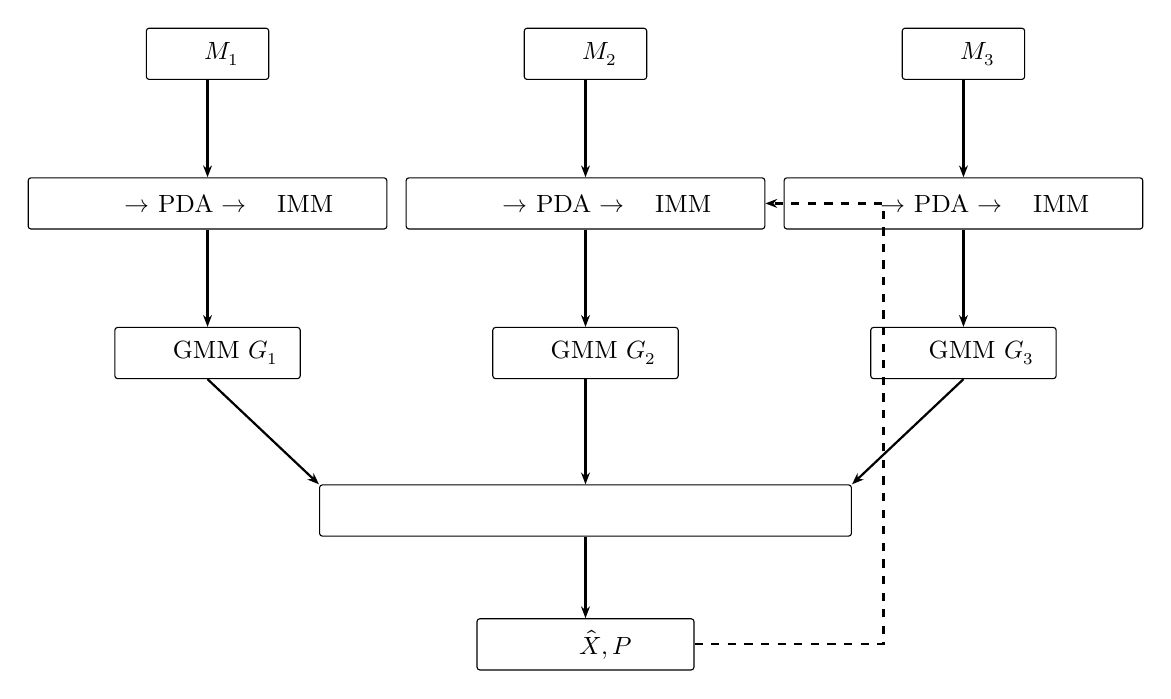
\begin{tikzpicture}[
  arr/.style={-{Stealth[length=1.5mm]}, thick},
  fb/.style={-{Stealth[length=1.5mm]}, thick, dashed},
  bn/.style={draw, rounded corners=1pt, align=center, font=\small,
             inner sep=2.2pt, minimum height=6.5mm, text width=14mm},
  bw/.style={draw, rounded corners=1pt, align=center, font=\small,
             inner sep=2.2pt, minimum height=6.5mm, text width=44mm}]
\foreach \i/\x in {1/0, 2/4.8, 3/9.6} {
  \node[bn] (m\i) at (\x,2.9) {无人机 $M_{\i}$};
  \node[bw] (p\i) at (\x,1.0) {双通道门控 $\to$ PDA $\to$ 本地 IMM};
  \node[bn, text width=22mm] (g\i) at (\x,-0.9) {局部后验 GMM $G_{\i}$};
  \draw[arr] (m\i) -- (p\i);
  \draw[arr] (p\i) -- (g\i);
}
\node[bw, text width=66mm] (fu) at (4.8,-2.9) {分布式多模型融合（具体配置见正文）};
\draw[arr] (g1.south) -- (fu.north west);
\draw[arr] (g2.south) -- (fu.north);
\draw[arr] (g3.south) -- (fu.north east);
\node[bn, text width=26mm] (gl) at (4.8,-4.6) {全局估计 $\hat{X},\boldsymbol{P}$};
\draw[arr] (fu) -- (gl);
\draw[fb] (gl.east) -- ++(2.4,0) |- (p2.east);
\node[font=\scriptsize, rotate=90, anchor=south] at (7.6,-1.8) {估计级反馈};
\end{tikzpicture}
\caption{多平台协同状态估计与分布式跟踪总体框架}
\label{fig:framework}
\end{figure}

框架中的信息交互分为两类：其一，为完成协同一致性检验，各机广播自身候选量测的角度与多普勒数值及检验统计量（量测级通信，每帧仅数个实数）；其二，为完成分布式融合与反馈，各机广播局部后验的估计量、协方差与分量权重（估计级通信）。整个框架不涉及原始信号或波形级数据交换，本文仅报告每帧参数负载，尚未验证包含报告频率、协议开销和链路条件的实际带宽需求。

综合第~3~节与本节的方法，完整的多平台协同状态估计流程如表~\ref{tab:algoflow} 所示。

\begin{table}[htbp]
\centering\small
\caption{多平台协同状态估计算法流程}\label{tab:algoflow}
\begin{tabular}{@{}>{\raggedleft\arraybackslash}p{0.09\linewidth}>{\raggedright\arraybackslash}p{0.86\linewidth}@{}}
\toprule
步骤 & 算法流程\\
\midrule
输入 & 三机候选量测集合\(\{Z_{k,i}\}\)，滤波初值，参数（表~\ref{tab:algo}）\\
1 & \textbf{for} \(k=1\to K\) \textbf{do}\\
2 & \quad 各机：由视线角量测三角定位得到几何位置\(P_g(k)\)；并以速度连续性正则化的跨机组合搜索（\(J_{\mathrm{tri}}\)按式~\eqref{eq:combo-tri}--\eqref{eq:combo-jtri}，速度惩罚按式~\eqref{eq:combo-vpen}；或纯角度几何/预测参照）选取参考候选（第~\ref{sec:t2}~节、3.3.7节）\\
3 & \quad 各机：计算距离-多普勒积分统计量\(Z_{i,m}(k)\)（式~\eqref{eq:t1-stat}）与跨机角度-距离投影统计量\(q_{i,m}\)（式~\eqref{eq:t2-stat}）\\
4 & \quad 各机：合成\(q^{\mathrm{tot}}_{i,m}\)（式~\eqref{eq:t2-total}），按式~\eqref{eq:dual-gate}的混合门控加权（\(q^{\mathrm{tot}}\le18.48\)内连续降权，超限置零）；若全部超限则保留\(q^{\mathrm{tot}}\)最小者\\
5 & \quad 各机：标准PDAF——门控、关联概率、等效量测（式~\eqref{eq:word-49}）与关联散布（式~\eqref{eq:pda-spread}）\\
6 & \quad 各机：IMM-EKF（CV/CA/Singer）更新，输出局部后验高斯混合\\
7 & \quad 融合中心：模式条件近似Chernoff融合（式~\eqref{eq:mode-cond}；对照口径\(w=0.5\)）+ 分量剪枝，输出全局估计\\
8 & \quad \textbf{if} \(k\bmod T_{\mathrm{fb}}=0\) \textbf{then} 全局估计按式~\eqref{eq:fb} 回灌各本地滤波器\\
9 & \textbf{end for}\\
输出 & 全局状态估计序列\(\{\hat{X}(k)\}\)\\
\bottomrule
\end{tabular}
\end{table}

\section{仿真与结果}\label{sec:results}


\subsection{场景、评价协议与信息条件}\label{sec:setup}
（2）\textbf{滤波器模型集与转移概率}：状态量为9维\([p_x,p_y,p_z,v_x,v_y,v_z,a_x,a_y,a_z]\)，模型集为CV/CA/Singer，初始模型概率均为1/3；转移概率矩阵取对角元素0.95、非对角元素0.025（传统VGPO主表沿用0.9/0.05，见第~\ref{sec:imm}~节与表~\ref{tab:algo} 注）；CV与CA模型按常数速度/常数加速度的离散白噪声形式构造过程噪声协方差，Singer模型按经典Singer公式\cite{singer1970}构造，其参数为机动频率\(\lambda=1/20\)~s\(^{-1}\)、最大机动加速度\(a_{\max}=8g\)（同时用作第~\ref{sec:fusion}~节处理(ii)机动包络先验标定的参数）、加速度取极大值的概率\(P_{\max}=0.5\)、加速度为零的概率\(P_0=0.5\)，加速度方差按\(\sigma_a^2=(a_{\max}^2/3)(1+4P_{\max}-P_0)\)确定。递推后验CRLB按式~\eqref{eq:word-13} 的量测模型与上述模型集以Kalman形式的信息递推计算。

（3）\textbf{候选量测生成与相关结构}：以目标真值状态生成量测后，每架无人机在每个时刻产生1条真实候选与\(N_J\)条干扰候选（三重/四重干扰下\(N_J=3/4\)，故\(M=4/5\)、跨机候选组合数为\(M^3=64/125\)）；干扰候选按第~\ref{sec:deception}~节的联合拖引模型生成。\textbf{主结果各表取\(\rho=0,\Delta R\equiv0\)}，即仅在多普勒通道叠加拖引偏置\(\Delta v_D(t)=f\!\left(\mathrm{mod}(t,T)/T\right)\cdot V\)（线性干扰取\(f(x)=x\)、抛物线干扰取\(f(x)=x^2\)），距离、俯仰角与方位角均与真实候选一致——该口径与既有工作可比，便于定位本文增量；\textbf{第~\ref{sec:robustness}~节则取\(\rho\in[0,1]\)}，并按式~\eqref{eq:rgpo-range} 叠加距离偏置、按式~\eqref{eq:rgpo-couple} 联动多普勒偏置，用于验证第~\ref{sec:theory}~节的双通道检验与可辨识性边界。两种口径共用同一场景、同一噪声模型与同一候选生成流程，仅干扰偏置不同。干扰通道在对称设定下对三架无人机同时施加（各机干扰参数相同），即每架无人机的候选集合相同。\textbf{候选噪声采用共享噪声模型}（式~\eqref{eq:shared-noise}）：同一平台同一时刻的全部候选使用同一份四维噪声实现，候选间差异只来自欺骗偏置。该假设的物理依据与理想化性质见式~\eqref{eq:shared-noise} 及其说明；若各候选独立加噪，门控内将出现\(M\)个相互独立的同一几何量测副本、可被标准PDA平均而人为压低误差，该口径伪影已在本文中排除。该假设的在线可检验性与违反时的退化见补充材料第~\ref{app:s}~节（相干共同臂的发散率由 0/30 升至 9/30）。为检验该对称假设，第~\ref{sup:ablation}~节补充了逐机干扰幅度为\([0.5,2.0,1.0]\)的非对称对照。

（4）\textbf{随机性与统计方法}：随机数按"世代$\times$流$\times$MC"分配。固定几何世代\texttt{main\_v1}中，第\(j\)次蒙特卡洛运行的场景、量测、候选与滤波器/PDA随机流基址分别为\(1000+j\)、\(2000+j\)、\(3000+j\)、\(4000+j\)；随机几何复核（\texttt{main\_jgeom\_v1}）复用同一组种子，仅把场景流真正用于几何抽样，故新旧结果可逐MC配对；锁箱（\texttt{lockbox\_v2}）使用独立基址，与历史流在整数种子与抽样指纹上均不相交。详细分配见补充材料第~\ref{sup:setup}~节，现场审计可运行\texttt{python -m src.seeds}。表~\ref{tab:rmse_main}、表~\ref{tab:ablation_fb}及第~\ref{sup:ablation}~节各表的配对差置信区间均由配对bootstrap给出（重采样10000次，随机种子0，取2.5\%与97.5\%分位数，以单次蒙特卡洛运行内的时间平均误差为配对单位）；除另有说明外，主结果、消融与非对称对照的蒙特卡洛次数均为50次。

为避免不同实验的信息前提被混读，表~\ref{tab:infocond} 汇总了全文各主要结果的\textbf{信息条件}（是否要求跨帧候选编号一致、是否要求跨平台编号一致、参考/锚定来源、是否使用真值标签、数据种子范围）。\textbf{正文各节不再重复说明同一组前提，凡结论均以该表所列条件为限}：例如第~\ref{sec:robustness}~节的联合拖引结果使用候选0作为参考，属\textbf{带身份参考的上界}；而第~\ref{sec:overall}~节--5.2.3节的传统VGPO结果不依赖任何真值标签。不同合同下的数值不可直接相减或互相外推。

主要量测噪声标准差为距离10 m、俯仰及方位各0.01 rad、多普勒20 m/s，采样间隔为0.02 s，目标采用4g S形机动。参数表中50次MC仅指传统VGPO主比较；T1/T2诊断、盲锚定、确认集和扩展确认集分别按各表样本数解释，不合并统计。完整场景坐标、平台航迹生成、初始化与随机流说明见补充材料第~\ref{sup:setup}~节。
\begin{table}[htbp]
\centering
\caption{算法参数}\label{tab:algo}
\begin{tabularx}{0.92\linewidth}{@{}p{0.16\linewidth}p{0.34\linewidth}X@{}}
\toprule
环节 & 参数 & 取值\\
\midrule
量测 & 机目距离噪声标准差（标称） & 10 m\\
量测 & 俯仰角/方位角噪声标准差（标称） & 0.01 rad / 0.01 rad\\
量测 & 多普勒速度噪声标准差（标称） & 20 m/s\\
双通道筛检（第~\ref{sec:theory}~节） & 积分窗长\(L\) / 合成门限（零假设经验校准） & \(L=100\)（2 s）/ \(\chi^2(7,0.99)=18.48\)（经验0.99分位18.15）\\
盲锚定（第~\ref{sec:association}~节） & 速度惩罚权重\(\gamma_v\) / 提前锁定门限 & 0.5 / 代价差\(\ge5\)且最佳\(\le8\) / T1预筛\(|Z|\le3\sigma_Z\)\\\midrule
一致性检验（对照口径，第~\ref{sec:single-channel}~节） & 白化统计量门限（零假设经验校准） & \(T=48\)（\(\chi^2_{3,0.99}=11.34\) 仅对应经验0.95分位）\\
PDA & 门控门限（马氏距离平方） & 16\\
IMM & 模型集 & CV / CA / Singer\\
IMM & 转移概率（对角/非对角） & 0.95 / 0.025（主配置）；0.9 / 0.05（旧口径）\\
融合 & 模式条件近似Chernoff（对照口径\(w=0.5\)） & 0.5（可行域[0.40,0.75]）\\
融合 & 分量剪枝阈值 & \(10^{-6}\)\\
反馈 & 反馈周期\(T_{\mathrm{fb}}\) / 膨胀系数\(\kappa\) & 5步（0.1 s）/ 1\\
统计 & 蒙特卡洛次数 & 50\\
\bottomrule
\end{tabularx}
\par\vspace{2pt}{\footnotesize 注：本稿不同结果链的 IMM 转移概率存在两组设置。自第~\ref{sec:end-to-end}~节起的端到端结果（RGPO/元组、锚定与确认、外部对比）由当前代码以 0.95/0.025 生成；传统VGPO 主表（表~\ref{tab:rmse_main}）及其同批消融沿用学位论文原稿口径 0.9/0.05（统一重跑脚本显式设置）。两组结果不跨表相减或互相外推。}
\end{table}

\begin{table}[htbp]
\centering
\caption{仿真参数（干扰通道对三架无人机对称施加，各机干扰参数相同）}\label{tab:parameters}
\begin{tabularx}{0.85\linewidth}{@{}Xcc@{}}
\toprule
定义 & 三重线性场景 & 四重混合场景\\
\midrule
第1重线性干扰周期/s & 5 & 6\\
第1重线性干扰范围/(m/s) & 16.7 & 16.7\\
第2重线性干扰周期/s & 8 & 9\\
第2重线性干扰范围/(m/s) & $-66.7$ & $-60$\\
第3重线性干扰周期/s & 12 & 11\\
第3重线性干扰范围/(m/s) & 50 & 73.3\\
第4重非线性（抛物线）干扰周期/s & — & 14\\
第4重非线性（抛物线）干扰范围/(m/s) & — & 50\\
\bottomrule
\end{tabularx}
\end{table}

第~\ref{sec:robustness}~节另引入距离-速度联合拖引参数（见第~\ref{sec:deception}~节）：运动学自洽混合系数\(\rho\in\{0,0.5,0.9,1\}\)、距离拖引率\(\dot{\Delta R}=50\) m/s、拖引起始时刻\(t_0=10\) s、逐机系数\(\eta_i\)取\([1,1,1]\)（共同模态）或\([1,0.6,1.35]\)（差分模态）。主结果各表仍按\(\rho=0,\Delta R\equiv0\)的传统VGPO口径给出，以保证与既有工作可比；两种口径共用同一场景、同一量测噪声与同一候选生成流程。

\begin{table}[htbp]
\centering
\caption{各结果的信息条件（“是”=该方法显式依赖该条件；“真值标签”=使用“哪条是真实回波”）}\label{tab:infocond}
\small
\resizebox{\textwidth}{!}{%
\begin{tabular}{@{}lccccc@{}}
\toprule
结果/表 & 跨帧编号一致 & 跨平台编号一致 & 参考/锚定来源 & 使用真值标签 & 数据种子\\
\midrule
表~\ref{tab:assoc} 跨帧身份 & 是 & 是（对角） & T1无需 / combo需 & 否 & 0$\sim$19\\
表~\ref{tab:rmse_main} 主RMSE & 否 & 否 & 无 & 否 & 0$\sim$49\\
表~\ref{tab:t1roc} T1检出 & 是（窗内同一候选） & 不适用 & H0池用候选0 & 是（仅H0） & 0$\sim$19\\
表~\ref{tab:t2sens} T2灵敏度 & 否（单帧） & 否 & 候选0 & 是 & 0$\sim$19\\
表~\ref{tab:rho-audit} \(\rho\)审计 & 是（窗内同一候选） & 不适用 & 无（偏置显式构造） & 是（仅H0标定） & 0$\sim$49\\
表~\ref{tab:rgpo_main} 端到端上界 & 否 & 不适用 & 候选0 & 是 & 0$\sim$49\\
表~\ref{tab:anchor} \texttt{index} & 是 & 是 & 候选0 & 是 & 0$\sim$19\\
表~\ref{tab:anchor} \texttt{combo+v} & 是（T1窗） & 是（对角） & combo & 否 & 0$\sim$19\\
表~\ref{tab:jointdrag-fusion} 前后端串联 & 是 & 是（对角） & \texttt{combo+v} & 否 & 0$\sim$19\\
表~\ref{tab:heldout} 确认集 & 是 & 是 & 同表~\ref{tab:anchor}/\ref{tab:jointdrag-fusion} & 否 & 100$\sim$119\\
表~\ref{tab:extcmp}--\ref{tab:extsel} 外部对比 & 是（T1窗，本文方法） & 是（对角，本文方法） & \texttt{combo+v} & 否 & 0$\sim$19 / 100$\sim$119\\
\bottomrule
\end{tabular}}
\par\vspace{2pt}
{\footnotesize 注：\texttt{combo+v} 的T1预筛使用$[k{-}L,k]$内同一候选的积分，故跨帧编号一致是硬前提；对角组合$(m,m,m)$进一步要求跨平台编号一致。全组合$(m_1,m_2,m_3)$用于单历元参考锚定（第~\ref{sec:t2}~节）与其端到端对照（表~\ref{tab:anchor} 的\texttt{combo}行）；\texttt{combo+v} 的跨帧累积与前后端串联（本表最后两行）使用对角组合。}
\end{table}

事件起点条件：表中以\texttt{combo+v}为前端的盲锚定、前后端串联及相应确认结果均使用已知起点与拖引前速度参考；这不等于未知起点下的验证。T1/T2诊断的窗口及零假设池按各自实验设置，不能与端到端身份输入混同。


元组扩展的信息条件与上表主配置分开：其跨平台编号可置换，但 T1 仍要求跨帧本地身份连续，事件起点的未知性未独立验证；数据种子为复用的 300--399。表~\ref{tab:tuple} 给出四种候选级判据配置的同批对照，结论是该扩展未带来改进（第~\ref{sec:tuple-results}~节）。表~\ref{tab:suppression}为300--349的真实回波移除压力测试，无真实候选，选真率不定义。




\subsection{可辨识性与检验性能验证}\label{sec:test-results}
本节验证第~\ref{sec:theory}~节的两个检验及其可辨识性边界。除特别说明外，干扰按第~\ref{sec:deception}~节的联合拖引模型生成：三重通道，拖引率\(\dot{\Delta R}=50\) m/s，拖引起始时刻\(t_0=10\) s，混合系数\(\rho\)与逐机系数\(\eta_i\)按各表设定；T1积分窗长\(L=100\)（2 s），T2与T1按式~\eqref{eq:t2-total} 合成，门限取\(\chi^2(7,0.99)=18.48\)；蒙特卡洛次数20（T1/T2诊断）或50（端到端）。



\subsubsection{T1检验性能与失配抵消}\label{sec:test-t1}
\noindent\textbf{检验一的可分辨边界}\quad 表~\ref{tab:t1roc}给出T1在虚警率固定为1\%时的检出率。可见在\(\rho=0\)（非相干）下检出率随拖引率与窗长单调上升：\(T=5\) s时\(\dot{\Delta R}=20\) m/s已达1.000，而\(\dot{\Delta R}=5\) m/s仍有0.170；在\(\rho=1\)（相干）下，全部\(\dot{\Delta R}\)与\(T\)组合的检出率恒为0.010，即\textbf{完全等于虚警底}——这与式~\eqref{eq:t1-mean} 的恒等式性质一致，而非灵敏度不足。图~\ref{fig:rgpo_t1}(b)给出干扰候选的\(|Z|/\sigma_Z\)随拖引率的变化（曲线参数为窗长）：解析式~\eqref{eq:t1-var} 给出的标准差与实测的相对偏差为0.3\%\(\sim\)1.6\%（与有限样本标准差估计的抽样误差同量级，\(n\approx4000\)）。对混合系数\(\rho\)的细扫（\(\dot{\Delta R}=20\) m/s、\(L=250\)）给出\(\rho=0,0.25,0.5,0.75,0.9,1\)时的检出率为0.909、0.615、0.261、0.057、0.017、0.010，随\((1-\rho)\)单调下降；\(\rho=0.25\)时仍有0.615，说明部分相干拖引比完全相干更接近可检，但已明显低于非相干。

\begin{table}[htbp]
\centering
\caption{检验一（距离-多普勒积分一致性）的检出率（虚警率1\%，MC=20）}\label{tab:t1roc}
\begin{tabular}{@{}cccccc@{}}
\toprule
\(\dot{\Delta R}\)/(m$\cdot$s$^{-1}$) & \(T=0.5\) s & \(T=1\) s & \(T=2\) s & \(T=5\) s & \(\rho=1\)（任意\(T\)）\\
\midrule
5   & 0.010 & 0.015 & 0.029 & 0.170 & 0.010\\
10  & 0.012 & 0.030 & 0.104 & 0.743 & 0.010\\
20  & 0.023 & 0.130 & 0.530 & 1.000 & 0.010\\
50  & 0.168 & 0.829 & 1.000 & 1.000 & 0.010\\
100 & 0.779 & 1.000 & 1.000 & 1.000 & 0.010\\
\bottomrule
\end{tabular}
\end{table}

\begin{figure}[htbp]
\centering
\includegraphics[width=0.74\linewidth]{latex/media/fig_rgpo_t1.png}
\caption{检验一的检出率与信噪比：(a) 虚警率1\%下的检出率随拖引率与积分窗长的变化，实线为\(\rho=0\)、虚线为\(\rho=1\)；(b) 干扰候选的\(|Z|/\sigma_Z\)随拖引率的增长（\(\rho=0\)，曲线参数为窗长），点线为3\(\sigma\)参考}
\label{fig:rgpo_t1}
\end{figure}

失配抵消对照见补充材料表~\ref{tab:rho-audit}：线性抵消与零均值失配均回到虚警底。因此检出率随\(\rho\)变化只能解释为该参数化下的净失配变化，不是信号级相干性的独立证据。


\subsubsection{T2、聚焦分量与门限标定}\label{sec:test-t2}
\noindent\textbf{检验二的可分辨边界}\quad 表~\ref{tab:t2sens}给出T2对单机距离偏置的响应。零假设下\(q\)的实测均值为5.94（理论\(\chi^2(6)\)均值为6），虚警率1.7\%，说明统计量口径正确；随偏置增大，检出率由\(\Delta R=7\) m的0.017升至\(\Delta R=175\) m的1.000，90\%检出对应约90 m（按非中心卡方模型对同一组检出率做单参数拟合；对粗网格线性内插会给出110 m，二者差异见第~\ref{sec:t2}~节(iii)与表~\ref{tab:drmin}）。需要说明，该门限是\textbf{本构型}（机间视线张角约19.6\(^\circ\)，评估时刻机目距离已缩至6.4--9.1 km）下的结果，随几何变化见下文（3）。

\begin{table}[htbp]
\centering
\caption{检验二（跨机角度-距离联合一致性）对单机距离偏置的响应（MC=20）}\label{tab:t2sens}
\begin{tabular}{@{}lcccccc@{}}
\toprule
\(t=14\) s处\(\Delta R\)/m & 7 & 17.5 & 35 & 70 & 175 & 350\\
\midrule
干扰候选\(q\)均值 & 6.1 & 7.1 & 10.6 & 24.6 & 122.4 & 472.1\\
检出率 & 0.017 & 0.067 & 0.167 & 0.633 & 1.000 & 1.000\\
\bottomrule
\end{tabular}
\end{table}

单历元ROC直接量化了降维收益：以\(\chi^2(1,0.99)=6.63\)为门限，\(q^{\mathrm{GLRT}}\)的90\%检出边界为\textbf{73 m}（非中心卡方模型拟合；80 m处实测0.867、90 m处0.983），而\(q\sim\chi^2(6)\)在16.81门限下为\textbf{90 m}（同为模型拟合；100 m处0.833、120 m处0.967）。两值均比同一组检出率的线性内插（83/110~m）低，原因见（iii）与表~\ref{tab:drmin}，二者\textbf{实测}虚警率相同（60个样本中1次超限，即1.7\%；名义门限为1\%，样本量不足以区分二者）；35/70 m偏置下检出率为0.283/0.783对0.167/0.633。需要说明，该比较刻画的是\textbf{6自由度阈值与聚焦检验的差距}，不是“混合门控尚有未兑现的增益”：混合门控在门限内已由式~\eqref{eq:thm1-cancel}达到GLRT，故表~\ref{tab:rgpo_main}的端到端数据不需重跑；残余的7自由度截断只作用于门限边界处权重本已很小的候选。

\noindent\textbf{（iii）命题3（可辨识边界的半闭式表达）。}\quad
定理1 已给出 \(q^{\mathrm{GLRT}}_{i,m}\sim\chi^2(1,\lambda_i)\)，\(\lambda_i=(\boldsymbol M_\perp)_{ii}\Delta R_i^2\)。把“可辨识边界”定义为“在门限 \(g_{1-\alpha}\) 下达到检出力 \(1-\beta\) 所需的最小单机距离偏置”，则由非中心卡方的单调性直接得到
\begin{equation}
\Delta R_{\min,i}(k)=\sqrt{\lambda^*(\alpha,\beta)\,\big/\,(\boldsymbol M_\perp)_{ii}(k)},
\qquad
\Pr\bigl\{\chi^2_{d}(\lambda^*)>g_{1-\alpha}\bigr\}=1-\beta,
\label{eq:drmin}
\end{equation}
其中自由度 \(d\) 取 \(q^{\mathrm{GLRT}}\) 的 1 或 \(q_{i,m}\) 的 \(3N-3\)。\(\alpha=0.01\)、\(\beta=0.10\) 时 \(\lambda^*=14.88\)（\(d=1\)，\(g=6.635\)）与 \(23.18\)（\(d=6\)，\(g=16.812\)）。式~\eqref{eq:drmin} 把定理1 的代数结论转成一个几何可读的量：\((\boldsymbol M_\perp)_{ii}\) 是第 \(i\) 机距离方向在“位置平移可解释子空间”之外的能量份额，故视线越接近共线（命题1 的极限），该份额越小、边界越远。三点限定：(a) 这是线性化结果（固定 \(\boldsymbol H\)、白化残差），非线性量测下为工作点的一阶近似；(b) 只覆盖\textbf{单机偏置}假设，即检验二的逐候选设定；(c) 门限与检出力必须显式声明，不同口径的 \(\lambda^*\) 不可互比。因此该式的定位是：在给定几何、单机偏置与线性化工作点下给出所需 \(\Delta R\) 的\textbf{量级估计}，而不是“任意几何与任意偏置组合能否被分辨”的判决工具——表~\ref{tab:drmin} 只在单一时刻、单一几何上与拟合值核对（相对差1.6\%/3.3\%），跨几何的适用性未逐点验证；联合共模偏置的实际检出边界见表~\ref{tab:joint_boundary}，它首先由参照是否洁净决定。另有一条有利性质：由于 \(\boldsymbol M_\perp\boldsymbol H=\boldsymbol 0\)（数值上 \(\|\boldsymbol M_\perp\boldsymbol H\|/\|\boldsymbol M_\perp\|=7\times10^{-20}\)），锚点位置的一阶误差 \(\boldsymbol H\delta\) 在残差投影中被精确消去；实测锚点平移 10/50/100~m 只使 \(q\) 变化 0.13\%/0.69\%/1.5\%。因此式~\eqref{eq:drmin} 的边界不依赖参考位置（\(\hat{\boldsymbol P}_0\)）的精度。

表~\ref{tab:drmin} 在本稿场景的评估窗首帧（\(t=10.8\)~s、机目距离 7.6--10.4~km、视线张角 19.6\(^\circ\)）上核对式~\eqref{eq:drmin}：把 \(q\) 的实测检出率曲线用非中心卡方模型做\textbf{单参数拟合}（自由参数即 \((\boldsymbol M_\perp)_{ii}\)），90\% 检出边界为 73.1/89.6~m，与闭式预测 74.2/92.6~m 相差 1--4\%，拟合值与几何计算值之比为 1.03/1.07。需说明：若直接对同一组检出率（20--200~m，13 点）做线性内插，会得到 83/110~m 一类偏高的边界——曲线在 100--140~m 以上已饱和，线性内插系统性高估 90\% 点；本文按模型拟合值报告。

\begin{table}[htbp]
\centering\small
\caption{可辨识边界的半闭式预测与模型拟合（\(t=10.8\)~s，\(\alpha=0.01\)，检出力 0.90）}
\label{tab:drmin}
\footnotesize
\begin{tabular}{@{}lcccccc@{}}
\toprule
统计量 & \(d\) & 门限 & \(\lambda^*\) & 半闭式/m & 拟合/m & 相对差\\
\midrule
\(q^{\mathrm{GLRT}}\) & 1 & 6.635 & 14.88 & 74.2 & 73.1 & $+1.5\%$\\
\(q_{i,m}\) & 6 & 16.812 & 23.18 & 92.6 & 89.6 & $+3.3\%$\\
\bottomrule
\end{tabular}
\par\vspace{2pt}{\footnotesize 注：“半闭式”为式~\eqref{eq:drmin} 代入逐帧几何的 \((\boldsymbol M_\perp)_{ii}=2.70\times10^{-3}\)（\(\sigma_R=10\)~m 时的绝对值，即 \(0.27\,\sigma_R^{-2}\)）；“拟合”为对实测检出率曲线（8 个偏置点；输入产物见补充材料E）单参数拟合的结果；相对差按（闭式\(-\)拟合）/拟合。}
\end{table}

\noindent\textbf{推论3.1（共模偏置的边界）}\quad
若三机被\textbf{同幅}偏置（每平台 \(\Delta R\)），联合偏置向量为
\(\Delta\boldsymbol b=\Delta R\,\boldsymbol 1=\sqrt N\,\Delta R\,\boldsymbol e\)，故
\begin{equation}
\lambda_J=\Delta\boldsymbol b^{\mathrm T}\boldsymbol M_\perp\Delta\boldsymbol b
=N\,\Delta R^2\,\boldsymbol e^{\mathrm T}\boldsymbol M_\perp\boldsymbol e
=\Delta R^2\,\boldsymbol 1^{\mathrm T}\boldsymbol M_\perp\boldsymbol 1 .
\label{eq:commom-lambda}
\end{equation}
这里 \(\boldsymbol e=\boldsymbol 1/\sqrt N\) 只是单位方向，\(\boldsymbol 1^{\mathrm T}\boldsymbol M_\perp\boldsymbol 1\)
才是"每平台偏置 1~m"对应的二次型（二者相差因子 \(N=3\)；单机情形 \(N=1\) 时退化为 \((\boldsymbol M_\perp)_{ii}\Delta R_i^2\)，
与第~\ref{sec:test-geometry}~节单机情形的 \((\boldsymbol M_\perp)_{ii}\Delta R_i^2\) 一致）。本稿构型 \(t=14\)~s 下 \(\boldsymbol e^{\mathrm T}\boldsymbol M_\perp\boldsymbol e\approx6.8\times10^{-6}\)~m\(^{-2}\)
（\(\sigma_R=10\)~m），即 \(\boldsymbol 1^{\mathrm T}\boldsymbol M_\perp\boldsymbol 1\approx2.0\times10^{-5}\)~m\(^{-2}\)：
取 \(d=1\)（\(\lambda^*=14.88\)）得 \textbf{\(\Delta R_{\min}\approx0.86\)~km}，
取 \(d=6\)（\(\lambda^*=23.18\)，与联合表同口径）得 \textbf{\(\approx1.07\)~km}。
即\textbf{共模偏置需接近公里量级才可被一阶检出}，位于第~\ref{sec:test-geometry}~节表~\ref{tab:joint_boundary}
（1000--3000~m，每平台口径）区间的下端，二者同量级。这与 第~\ref{sec:test-geometry}~节的结论一致，也说明“联合距离-速度抗欺骗”的难点在参照洁净度，而非统计量复杂度。

\begin{table}[htbp]
\centering
\caption{单帧虚警率与轨迹级虚警率（独立零假设种子 MC=100$\sim$119；T1 共 3600 帧、T2 与合成量共 10800 个平台-帧、20 条轨迹；轨迹级指标指“整条轨迹至少一次超限”的比例；末列为按独立帧二项模型 $1-(1-\alpha)^{K}$ 给出的期望值）}\label{tab:far}
\small
\begin{tabular}{@{}lccccc@{}}
\toprule
统计量 & 名义门限 & 帧级 FAR [95\%CI] & 单轨迹 FAR 范围 & 轨迹级$\ge1$次超限 & 独立帧预测\\
\midrule
T1 & $2.630\sigma_Z$ & 0.0075 [0.005,0.010] & 0$\sim$0.0222 & 15/20 & 0.836\\
T2 & 16.81 & 0.0069 [0.0055,0.0085] & 0$\sim$0.0167 & 14/20 & 0.996\\
$q^{\mathrm{tot}}$ & 18.48 & 0.0100 [0.0082,0.0119] & 0.0019$\sim$0.0167 & 20/20 & 0.996\\
\bottomrule
\end{tabular}
\end{table}

帧级名义1\%门限不构成整条轨迹的1\%误警保证。独立零假设种子上，T1、T2与合成量分别有15/20、14/20与20/20条轨迹至少一次超限；详细统计与相关性解释见补充材料第~\ref{sup:gate}~节。

\textbf{盲参考条件下的条件虚警率}：上述校准使用“已知参考候选身份”的口径。为检验数据依赖选择是否改变零分布，在同一批种子上比较纯角度三角定位锚定（\texttt{geo}，不使用任何身份标签）与身份锚定（\texttt{index}）：在距离未被拖引的臂上两者均为 \textbf{1.20\%}（名义 1\%，$n=4500$）；在距离被拖引的非相干臂上，geo 的整体“误剔除率”升至 51.4\%，但\textbf{其中 geo 仍选中真候选的帧上只有 0.99\%}，其余 66.3\% 的帧是 geo 锚到了假候选（此时判真候选不一致属于正确检测，不是虚警）。即：\textbf{条件分布未因选择事件而偏移}，盲锚定的高拒绝率来自锚定失败而非虚警膨胀。数据与分解脚本见补充材料“盲参考条件下的 T2 虚警率”一节。


\subsubsection{几何与参考条件对检测边界的影响}\label{sec:test-geometry}
量级关系的数值验证：在锥形几何（仰角20\(^\circ\)、方位\(\pm\Delta\theta/2\)与0）上，对"每机距离\(+\Delta R\)、角度不变"的幽灵候选，以三维状态为未知量对9维量测做加权最小二乘，得最小白化残差\(d_{\min}\)。图~\ref{fig:prop1_scaling}给出\(\sqrt{d_{\min}}\)对\(\Delta R\sin\Delta\theta_{\mathrm{LOS}}/(R\sigma_{\mathrm{ang}})\)的关系：过原点线性拟合斜率0.85（\(R^2=0.967\)），按张角与距离分组的斜率在0.68\(\sim\)1.14之间、随二者缓变——即上述\(O(\cdot)\)的常数是几何依赖的\(O(1)\)量，量级关系本身在\(2^\circ\sim40^\circ\)、6\(\sim\)12 km内成立。

\begin{figure}[htbp]
\centering
\includegraphics[width=0.62\linewidth]{latex/media/fig_prop1_scaling.png}
\caption{命题1量级关系的数值验证：\(\sqrt{d_{\min}}\)与\(\Delta R\sin\Delta\theta/(R\sigma_{\mathrm{ang}})\)过原点线性（斜率0.85，\(R^2=0.967\)），分组斜率0.68--1.14随几何缓变}\label{fig:prop1_scaling}
\end{figure}

\noindent\textbf{编队几何的影响}\quad 图~\ref{fig:rgpo_geom}在合成几何上扫描机间视线张角\(\Delta\theta_{\mathrm{LOS}}\)（目标位于锥轴，平台置于半锥角\(\theta\)的锥面上），以90\%检出、1\%虚警为判据给出可分辨距离偏置\(\Delta R_{\min}\)。结果与直觉相反：\(\Delta\theta_{\mathrm{LOS}}\)由4.3\(^\circ\)增至51.3\(^\circ\)时\(\Delta R_{\min}\)由80 m升至350 m，即\textbf{基线越宽，单机距离偏置越难检出}。其机理是：3个距离对3个未知位置恰好定解，任何距离偏置都可被某个位置平移吸收，残差仅来自角度与该平移的不一致；窄基线使距离方程接近平行、解病态放大，单位偏置引起的位置平移更大，角度的可观测分量随之增大。这一趋势与角度定位精度对宽基线的需求相反，构成编队设计的显式权衡。图中共同与差分模态两条曲线按构造重合：式~\eqref{eq:t2-stat} 的逐候选假设只把第\(i\)机替换为候选\(m\)、其余两机仍取参考候选，故统计量与该两机的偏置幅度无关。

\begin{figure}[htbp]
\centering
\includegraphics[width=0.72\linewidth]{latex/media/fig_rgpo_geom.png}
\caption{编队几何对可分辨距离偏置的影响：横轴为机间视线张角，纵轴为满足90\%检出/1\%虚警的最小\(\Delta R\)}
\label{fig:rgpo_geom}
\end{figure}

\begin{figure}[htbp]
\centering
\includegraphics[width=0.80\linewidth]{latex/media/fig_rgpo_dk.png}
\caption{所设仿真轨迹上的动态可辨识性（20次蒙特卡洛中位与10/90带；图内“真实轨迹”指仿真真值轨迹，并非实测数据）：最大视线张角、视线矩阵条件数、\(d(110\,\mathrm m)\)与检验二统计量}\label{fig:rgpo_dk}
\end{figure}

图~\ref{fig:rgpo_dk}在本文仿真场景（表~\ref{tab:scene}）上逐帧复核上述结论。评估窗内三机最大视线张角为\(19.56^\circ\)--\(19.62^\circ\)（非23\(^\circ\)），视线矩阵条件数7.2--7.6；\(d(110\,\mathrm m)\)的中位由初始约4.3升至末段约7.4（距离收缩使\(R\sigma_{\mathrm{ang}}\)变小），\textbf{全窗均高于3\(\sigma\)}；真实候选的\(q_{T2}\)中位为5--6（与\(\chi^2(6)\)均值6一致），干扰候选的中位约在\(t=11.4\) s越过门限。这说明表~\ref{tab:t2sens}的边界（90 m）并非只在某一帧成立（图中取 110 m 作为诊断偏置，全窗均高于 3\(\sigma\)），且与图~\ref{fig:rgpo_geom}的12 km设计曲线在距离折算后自洽（19.6\(^\circ\)、12 km约140 m，按\(R\)折算至6.4--9.1 km约85--105 m）。

\noindent\textbf{混合系数与偏置模态的可辨识性地图}\quad 图~\ref{fig:rgpo_map}给出\(\rho\)由0增至1时两个检验的检出率。该读数在\textbf{固定失配波形、仅缩放幅度}的参数化下取得（\(v_j\equiv0\)，见(7)），应解释为净失配幅度减小的效应，而非“相干性”本身的物理效应。T1的检出率在\(\rho=0.9\)时已降至0.083、在\(\rho=1\)时降为0，而T2在全区间保持有效，二者并集在测试范围内恒为1.00。这与第~\ref{sec:single-channel}~节的命题1一致：相干拖引抹去T1赖以工作的距离--多普勒失配，只能由跨机差分分量提供可辨识性。

\begin{figure}[htbp]
\centering
\includegraphics[width=0.78\linewidth]{latex/media/fig_rgpo_map.png}
\caption{混合系数与偏置模态的可辨识性地图（\(\dot{\Delta R}=10\)与50 m/s）：T1在\(\rho\to1\)时失明，T2补位，二者并集保持有效}
\label{fig:rgpo_map}
\end{figure}

为量化这一差异，在合成圆锥几何（目标位于锥轴、\(R=12\) km、\(\sigma_R=10\) m、\(\sigma_\alpha=\sigma_\beta=0.01\) rad）上做100次蒙特卡洛：逐候选假设只替换第1架，联合假设同时替换三架；两者均以\(\chi^2(6,0.99)=16.81\)为门限，统计90\%检出所需的\(\Delta R\)。结果见表~\ref{tab:joint_boundary}与图~\ref{fig:rgpo_joint}。

\begin{table}[htbp]
\centering
\caption{逐候选假设与三机联合假设的90\%检出边界（100次蒙特卡洛，\(R=12\) km）}\label{tab:joint_boundary}
\begin{tabular}{@{}lcccccc@{}}
\toprule
最大视线张角 & \(4.3^\circ\) & \(8.7^\circ\) & \(17.3^\circ\) & \(25.9^\circ\) & \(34.5^\circ\) & \(51.3^\circ\)\\
\midrule
逐候选\(\Delta R_{\min}\)/m & 80 & 80 & 120 & 200 & 200 & 350\\
三机联合\(\Delta R_{\min}\)/m & \(>3000\) & \(>3000\) & 3000 & 1800 & 1000 & 600\\
联合假设虚警率 & 0.00 & 0.00 & 0.01 & 0.01 & 0.01 & 0.01\\
\bottomrule
\end{tabular}
\end{table}

\begin{figure}[htbp]
\centering
\includegraphics[width=0.76\linewidth]{latex/media/fig_rgpo_joint.png}
\caption{逐候选假设与三机联合假设的90\%检出边界：联合假设在窄角下3 km内仍达不到90\%，对应命题1的径向幽灵}\label{fig:rgpo_joint}
\end{figure}

表~\ref{tab:joint_boundary}给出三点。其一，\textbf{逐候选边界与图~\ref{fig:rgpo_geom}逐点一致}（80/80/120/200/200/350 m），说明两组实验的生成器与统计量口径相同。其二，\textbf{三机联合假设难2.5--25倍}：同样90\%检出，联合假设需600--3000 m；在\(4.3^\circ\)--\(8.7^\circ\)的窄角下，3 km仍达不到90\%。这正是命题1的"径向幽灵"——三机距离同时增加同一个\(\Delta R\)，可被一个沿共同视线平移的虚拟目标解释，角度残差只有\(O(\Delta R\sin\Delta\theta_{\mathrm{LOS}}/(R\sigma_{\mathrm{ang}}))\)。其三，\textbf{联合假设的零假设虚警率为0--1\%}，说明\(\chi^2(6)\)门限本身没有问题，差异来自假设的可行域而非门限失配。

因此，本文的"90 m"应严格表述为\textbf{逐候选、且候选集中存在干净参照}时的边界；当干扰源完成三机协同拖引时，候选集中不再有未被替换的参照，已超出"候选集中存在真实回波"的本文假设；该情形超出本文假设；本文没有建立对任意单历元检验均不可能可靠区分的普遍结论。这一区分同时解释了为何本文不把"联合距离-速度抗欺骗"本身作为创新主张：真正决定检测能力的是\textbf{参照的洁净度}，而不是统计量的复杂度。



\subsubsection{任意\(N\)平台分解的数值验证}\label{sec:test-n}
图~\ref{fig:theorem1-verification}给出\(q^{\mathrm{GLRT}}_{i,m}\)在\(N=3,4,5\)下的边缘分布。三个配置的Kolmogorov-Smirnov检验\(p\)值分别为0.582、0.068、0.991，\textbf{均未拒绝}\(\chi^2(1)\)；但“未拒绝”只表示当前样本量下未发现显著偏离，不等同于证明定理。定理1'还包含另两项可检验的结论——剩余分量服从\(\chi^2(\nu)\)、两个分量相互独立——且需覆盖\(r<3\)的秩亏情形。表~\ref{tab:thm1-verify}用独立抽样同时检验这三点。

\begin{figure}[htbp]
\centering
\includegraphics[width=\textwidth]{fig1_theorem1_verification.pdf}
\caption{定理1'的一维分量验证：\(N=3,4,5\)一般配置下\(q^{\mathrm{GLRT}}\)的样本分布与\(\chi^2(1)\)理论密度（KS检验\(p=0.582/0.068/0.991\)，均未拒绝）。剩余分量的自由度与两分量独立性见表~\ref{tab:thm1-verify}。}
\label{fig:theorem1-verification}
\end{figure}

\begin{table}[htbp]
\centering
\caption{定理1'的完整数值验证（每配置4000次抽样；白化残差\(\widetilde{\boldsymbol r}\sim\mathcal N(\boldsymbol 0,\boldsymbol I)\)，\(\boldsymbol H\)为距离-角度联合雅可比）}\label{tab:thm1-verify}
\small
\begin{tabular}{@{}lcccccccc@{}}
\toprule
配置 & \(r\) & \(\nu\) & \(\mathbb E[q^{\mathrm{GLRT}}]\) & \(\operatorname{Var}[q^{\mathrm{GLRT}}]\) & \(\mathbb E[q_{-i}]\) & \(\operatorname{Var}[q_{-i}]\) & \(\rho(q^{\mathrm{GLRT}},q_{-i})\) & KS \(p\)（\(q_{-i}\)）\\
\midrule
\(N=3\) & 3 & 5 & 0.997 & 1.891 & 4.911 & 9.569 & \(-0.002\) & 0.204\\
\(N=4\) & 3 & 8 & 1.023 & 2.103 & 8.026 & 16.189 & \(+0.018\) & 0.830\\
\(N=5\) & 3 & 11 & 0.988 & 1.910 & 10.813 & 20.452 & \(-0.026\) & 0.058\\
\(N=3\)（秩亏） & 2 & 6 & 0.970 & 2.011 & 5.988 & 12.120 & \(-0.002\) & 0.458\\
\midrule
理论值 & — & — & 1 & 2 & \(\nu\) & \(2\nu\) & 0 & —\\
\bottomrule
\end{tabular}
\par\vspace{2pt}{\footnotesize 注：秩亏行为人为将\(\boldsymbol H\)的第三列置零（\(z\)方向不可观）所得，用于检验自由度公式在\(r<3\)下的形式；本稿实际几何的\(\operatorname{rank}(\boldsymbol H)=3\)。三行的\(\mathbb E[q_{-i}]\)与\(\operatorname{Var}[q_{-i}]\)分别与\(\nu=5,8,11\)、\(2\nu=10,16,22\)吻合。表中KS \(p\)列为\(q_{-i}\sim\chi^2(\nu)\)的检验结果；\(q^{\mathrm{GLRT}}\sim\chi^2(1)\)的KS \(p\)为0.582/0.068/0.991（\(N=3/4/5\)，与图~\ref{fig:theorem1-verification} 同源），秩亏配置为0.227。\textbf{本表的作用边界}：抽样直接由白化残差\(\widetilde{\boldsymbol r}\sim\mathcal N(\boldsymbol 0,\boldsymbol I)\)生成，检验的是分解式与分布推导的\emph{数值实现一致性}，\textbf{不构成}对非线性仿真残差是否满足该标准正态前提的检验（前提的适用范围见补充材料A开头）；表中\(\rho\approx0\)是正交二次型理论的结果，\textbf{不单独作为两分量独立的证据}。}
\end{table}



\subsection{端到端性能与消融}\label{sec:end-to-end}


\subsubsection{总体虚假量测抑制表现}\label{sec:overall}
在三重线性与四重混合两种干扰场景下各进行$N_{\mathrm{MC}}=50$次独立蒙特卡洛仿真（无干扰基线亦为$N_{\mathrm{MC}}=50$次），表~\ref{tab:rmse_main}给出了各对比方法在位置、速度与加速度三个维度上的RMSE中位值以及（均值$\pm$标准差）统计结果，图~\ref{fig:err-curves}给出了位置误差随时间的变化曲线。主要结论如下：

\begin{table}[htbp]
\centering
\caption{各方法位置、速度与加速度RMSE统计对比（中位值[均值$\pm$标准差]，$\mathrm{MC}=50$）}
\label{tab:rmse_main}
\resizebox{\textwidth}{!}{%
\begin{tabular}{lcccccc}
\toprule
\multirow{2}{*}{跟踪方法} & \multicolumn{2}{c}{位置RMSE/m} & \multicolumn{2}{c}{速度RMSE/(m/s)} & \multicolumn{2}{c}{加速度RMSE/(m/s$^2$)}\\
\cmidrule(lr){2-3}\cmidrule(lr){4-5}\cmidrule(lr){6-7}
 & 三重线性 & 四重混合 & 三重线性 & 四重混合 & 三重线性 & 四重混合\\
\midrule
无门控基线 & 10.35[10.47$\pm$1.19] & 10.29[10.43$\pm$1.02] & 17.67[17.59$\pm$0.80] & 17.97[17.93$\pm$0.92] & 26.62[26.63$\pm$0.21] & 26.57[26.59$\pm$0.21]\\
集中式PDA & 10.69[10.75$\pm$0.87] & 10.73[10.71$\pm$0.83] & 20.77[20.77$\pm$1.03] & 21.16[21.16$\pm$1.18] & 29.65[29.65$\pm$0.96] & 30.07[30.07$\pm$1.24]\\
单机独立处理 & 26.57[26.94$\pm$4.76] & 25.17[25.98$\pm$2.42] & 38.03[37.65$\pm$2.82] & 37.26[37.28$\pm$2.63] & 31.68[31.97$\pm$1.36] & 31.99[32.08$\pm$1.27]\\
CI融合（无反馈，开环基线） & 12.74[13.08$\pm$2.58] & 11.87[13.02$\pm$2.98] & 21.32[21.40$\pm$1.80] & 20.78[21.56$\pm$2.40] & 26.05[26.09$\pm$0.79] & 26.04[26.10$\pm$0.96]\\
CI融合（有反馈） & 10.30[10.52$\pm$1.31] & 10.28[10.38$\pm$1.06] & 17.76[17.99$\pm$0.91] & 18.09[18.05$\pm$0.98] & 26.89[26.88$\pm$0.19] & 26.87[26.90$\pm$0.25]\\
本文方法（ACF+反馈） & 10.30[10.52$\pm$1.31] & 10.28[10.38$\pm$1.06] & 17.77[18.01$\pm$0.91] & 18.13[18.07$\pm$0.99] & 26.88[26.86$\pm$0.19] & 26.84[26.88$\pm$0.26]\\
本文方法（无反馈对照） & 12.72[13.07$\pm$2.58] & 11.86[13.01$\pm$2.98] & 21.05[21.12$\pm$1.75] & 20.63[21.29$\pm$2.33] & 25.69[25.62$\pm$0.64] & 25.71[25.68$\pm$0.71]\\
仅选真候选 & 10.39[10.54$\pm$1.29] & 10.29[10.40$\pm$1.04] & 17.85[18.08$\pm$0.90] & 18.15[18.08$\pm$0.95] & 26.89[26.90$\pm$0.21] & 26.84[26.86$\pm$0.25]\\
\bottomrule
\end{tabular}}
\vspace{2pt}
\parbox{\textwidth}{\footnotesize 注：\textbf{本表不构成“本文在位置与速度上全面最优”的证据}。位置维：四重混合为本文与 CI+反馈并列最优（10.38~m），三重线性则是“无门控基线”更低（10.47~m 对本文 10.52~m，差 0.05~m）；速度维：两场景的最优值均属于“无门控基线”（17.59/17.93~m/s，本文为 18.01/18.07~m/s）。本表支持的是三点：（i）反馈相对无反馈有明确收益（位置主效应 $-2.56/-2.64$~m，见表~\ref{tab:factorial}）；（ii）CI 与 ACF 的差异不足 0.01~m；（iii）在传统VGPO 这类\textbf{无相干距离偏置}的场景下，门控与否对位置精度影响很小（$\le0.05$~m），本文方法的代价主要体现在速度维。带相干距离偏置时的收益须看表~\ref{tab:rgpo_main}与表~\ref{tab:extcmp}，不能由本表外推。“仅选真候选”行为是\textbf{已知候选身份下的单候选参考}（不是所有软融合估计器的精度上界，见第~5.5节），不计入方法比较；加速度维各法的差异不构成方法优劣的依据。}
\end{table}

\begin{figure}[htbp]
\centering
\includegraphics[width=0.49\linewidth]{latex/media/fig_err_3linear.png}
\hfill
\includegraphics[width=0.49\linewidth]{latex/media/fig_err_4mixed.png}
\caption{两种干扰场景下位置误差随时间变化（每幅左：位置RMSE；右：位置误差中位；场景由子图标题标注）}
\label{fig:err-curves}
\end{figure}

表~\ref{tab:rmse_main}属于传统VGPO合同；表~\ref{tab:rgpo_main}属于联合拖引且带身份参考的上界合同，不能跨表直接计算增益。完整逐项比较保留在补充材料第~\ref{sup:overall}~节。
\begin{table}[htbp]
\centering
\caption{双通道混合门控的端到端效果（位置RMSE，m；50次蒙特卡洛；配对bootstrap 10000次；混合列以候选0为参考，含真值身份信息，属已知身份参考）}\label{tab:rgpo_main}
\small
\begin{tabular}{@{}lcccccc@{}}
\toprule
干扰模态 & PDA均值 & 中位 & 90\%分位 & 混合均值 & 中位 & 90\%分位\\
\midrule
传统VGPO & 10.75 & 10.69 & 11.64 & 10.82 & 10.73 & 12.25\\
非相干 & 10.79 & 10.66 & 11.83 & 10.84 & 10.82 & 11.74\\
相干·共同 & 26.63 & 11.23 & 124.81 & 11.06 & 11.01 & 11.99\\
相干·差分 & 11.59 & 11.64 & 12.72 & 11.30 & 11.41 & 12.48\\
\bottomrule
\end{tabular}
\end{table}

由表~\ref{tab:rgpo_main}可得两点。其一，\textbf{真回波在场的传统VGPO与非相干两臂未观察到显著平均差异}：传统VGPO与非相干两臂的配对差分别为$+0.07$ m（95\%CI $[-0.02,+0.17]$）与$+0.05$ m（$[-0.05,+0.14]$），均含零；相干差分臂改善$0.29$ m（$[0.19,0.39]$）。其二，\textbf{相干共同模态下收益集中在尾部}：中位值由11.23 m变为11.01 m（基本不变），而90\%分位由124.81 m降至11.99 m、发散样本（位置RMSE$>50$ m）由6/50降至0/50，均值改善$15.57$ m（$[4.97,27.73]$）。因此该模块的定位应是\textbf{抑制长尾}而非提升典型精度，这与第~\ref{sec:feedback}~节周期反馈的作用模式一致——两者攻击同一失效模式。

需要强调，0/50 不表示发散概率为零：按独立伯努利模型，50 次试验零发散的单侧 95\% 置信上界约为 5.8\%。本文所列配对 bootstrap 区间对应均值差，未对中位数差与90\%分位差作同等检验，故"p90 由 124.81 m 降至 11.99 m"应理解为点估计而非显著性结论。此外，表~\ref{tab:rgpo_main}为 50 次蒙特卡洛（上界参考），表~\ref{tab:anchor}为 20 次蒙特卡洛（锚定对照），两者不可跨表计算增益；加入式~\eqref{eq:combo-vpen}的速度惩罚后，盲锚定（不使用真值标签）为11.16 m，与表~\ref{tab:anchor}的\texttt{index}上界11.17 m的配对差95\%CI跨零；由于MC规模不同（50对20），仍不将其与表~\ref{tab:rgpo_main}的11.06 m直接等同。

最后需要指出兜底策略的影响。若全剔除时改为全部放行，相干共同模态的位置RMSE为100.71 m；保留\(q^{\mathrm{tot}}\)最小者为25.83 m；按漏检处理为53.15 m（MC=6）。三者的量级差异说明兜底策略是方法设计的一部分，而非实现细节，这与第~\ref{sec:pda}~节的结论一致。



\subsubsection{硬门控与混合门控}\label{sec:hard-mixed}
接入关联时采用式~\eqref{eq:dual-gate} 的\textbf{混合门控}（本质是\textbf{启发式关联权重}，不是贝叶斯最优后验）：门限内按统计量幅值连续降权，门限外一律置零。它保留了硬门限的统计边界，同时避免硬门控在拖引初期"门限内全放行"的漏放问题。50次蒙特卡洛的主合同对比（同一批种子、同一候选集；参考候选取候选0，即上界）给出：相干共同臂位置RMSE由硬门控的16.96 m降至11.06 m（配对差\(+5.89\) m，95\%CI \([+0.27,+14.58]\)，基于混合臂自身的逐MC配对bootstrap），90\%分位由12.84 m降至11.99 m，发散样本（RMSE\(>50\) m）由3/50降至0/50；需要交代该均值差的构成：两臂中位值分别为11.04 m与11.01 m，5.89 m的均值差由硬门控3个\(>50\) m样本（53.6、58.4、212.0 m）贡献，剔除其中最大的一个后均值差降为2.09 m，逐MC配对\(t\)检验\(p=0.15\)、Wilcoxon符号秩检验\(p=7.2\times10^{-5}\)（同一批50个种子复算）。因此该对照支持的是“混合门控抑制尾部”，不支持“混合门控在典型工况下更准”；相干差分臂由11.51 m降至11.30 m（\(+0.21\)，\([+0.12,+0.30]\)）；传统VGPO与非相干臂无显著差异。协方差一致性同向：硬门控在传统VGPO的ANEES3为7.05（覆盖率0.644）、相干共同臂为36.24，混合门控分别为5.04（0.798）与3.72（0.907），50次蒙特卡洛的配对bootstrap置信区间均不含零。机理是硬门限在拖引开始后2\(\sim\)4 s内仍放行56\%\(\sim\)62\%的假候选（其\(q^{\mathrm{tot}}\)中位数13.7\(\sim\)15.8，低于18.48），连续降权把其相对权重压到0.016\(\sim\)0.056；后期\(\Delta R\)拉开后两者等价。100次蒙特卡洛复核给出同向结论：传统VGPO与非相干臂的"硬减混合"配对差为\(+0.00\)（\([-0.04,+0.04]\)）与\(+0.02\)（\([-0.03,+0.06]\)），相干共同与差分臂为\(+5.87\)（\([+0.59,+13.63]\)）与\(+0.59\)（\([+0.21,+1.30]\)），上述结果仅描述所测试场景中的差异；区间包含零的比较不能据此解释为已证明等效或非劣。需要说明，混合门控仍被限制在\(q^{\mathrm{tot}}\le18.48\)的统计边界内，并非无约束的二次计权；若场景或噪声口径改变，门限应按本节程序重新标定。



\subsubsection{融合与反馈的作用分离}\label{sec:fusion-ablation}
\textbf{融合方式与反馈的2×2因子对照（表~\ref{tab:factorial}）}：为分离估计级融合方式与反馈机制的独立贡献及其交互，在三重线性与四重混合场景下各做$\{$CI\,/\,ACF$\}\times\{$无反馈\,/\,有反馈$\}$的2×2对照（MC=50，逐种子配对）。结果表明：\textbf{反馈是位置与速度精度的主要来源}——位置主效应 $-2.556$~m（95\%CI $[-3.172,-1.976]$，三重线性）与 $-2.641$~m（$[-3.278,-2.028]$，四重混合），速度主效应 $-3.260$ 与 $-3.365$~m/s，均不跨零；但\textbf{加速度维相反}，反馈使其增大 $+1.019$ 与 $+0.998$~m/s$^2$，即位置/速度的提升以加速度平滑性为代价。\textbf{CI 与 ACF 的差异极小}：位置融合主效应 $-0.0083$ 与 $-0.0056$~m，速度 $-0.132$ 与 $-0.127$~m/s，因样本量大而统计可区分，但相对效应不足 0.1\%，不作非劣效结论。位置交互项为 $+0.0067$ 与 $+0.0089$~m：\textbf{置信区间不跨零}（$[+0.0016,+0.0120]$、$[+0.0028,+0.0158]$），但与反馈主效应相比量级不足 1/300，实际可忽略；速度交互 $+0.303/+0.293$~m/s、加速度交互 $+0.448/+0.390$~m/s$^2$。因此两因素在主效应层面可加，交互虽统计显著但无实际意义。

\begin{table}[htbp]
\centering
\caption{融合方式与估计级反馈的2×2因子对照（单元位置RMSE 均值，单位：m；主效应与交互项为配对差，bootstrap 10000，MC=50）}
\label{tab:factorial}
\resizebox{\textwidth}{!}{%
\begin{tabular}{lcccccccc}
\toprule
\multirow{2}{*}{场景} & \multicolumn{4}{c}{单元位置RMSE 均值/m} & \multicolumn{3}{c}{主效应与交互项（95\%CI）}\\
\cmidrule(lr){2-5}\cmidrule(lr){6-8}
 & CI无反馈 & CI有反馈 & ACF无反馈 & ACF有反馈 & 反馈主效应 & 融合主效应 & 交互项\\
\midrule
三重线性 & 13.080 & 10.520 & 13.068 & 10.515 & $-2.556\ [-3.172,-1.976]$ & $-0.0083\ [-0.0111,-0.0056]$ & $+0.0067\ [+0.0016,+0.0120]$\\
四重混合 & 13.023 & 10.377 & 13.013 & 10.376 & $-2.641\ [-3.278,-2.028]$ & $-0.0056\ [-0.0083,-0.0027]$ & $+0.0089\ [+0.0028,+0.0158]$\\
\bottomrule
\end{tabular}}
\end{table}

模式条件ACF与CI在传统VGPO下的位置差异不足0.01 m，统计可区分而实际效应不足0.1\%；未做非劣效检验。反馈参数、融合顺序、奇异分量与非对称干扰等完整消融见补充材料第~\ref{sup:ablation}~节，本文主结果仍使用机动包络标定配置。表~\ref{tab:rmse_main}、表~\ref{tab:factorial} 与表~\ref{tab:consistency} 来自早期 F50/F60 链路，其原始产物未随本分支保留；本轮已用当前代码重建该链路的可执行版本并跑满 50 次蒙特卡洛，定性结论一致、绝对值存在 0.3$\sim$0.8~m 的系统差，详见补充材料补充材料“F50/F60 链路的重跑与三张表的口径切换”小节。两者\textbf{不可混用}。
\begin{table}[htbp]
\centering
\caption{联合拖引合同下前后端串联的位置RMSE（m，20次蒙特卡洛；前端统一为双通道混合门控+速度惩罚\texttt{combo+v}+T1预筛；配对差为逐MC bootstrap 95\%CI）}\label{tab:jointdrag-fusion}
\small
\resizebox{\textwidth}{!}{%
\begin{tabular}{@{}lccccc@{}}
\toprule
场景 & CI+反馈 & ACF+反馈（坍缩） & ACF+反馈（分模式） & ACF$-$CI [95\%CI] & 分模式$-$ACF [95\%CI]\\
\midrule
传统VGPO & 10.60 & 10.60 & 10.74 & $-0.003\ [-0.008,+0.002]$ & $+0.138\ [+0.092,+0.182]$\\
RGPO非相干 & 10.75 & 10.75 & 10.92 & $-0.004\ [-0.010,+0.002]$ & $+0.174\ [+0.101,+0.279]$\\
相干·共同 & \textbf{10.53} & \textbf{10.53} & 10.64 & $+0.000\ [-0.008,+0.008]$ & $+0.116\ [+0.072,+0.160]$\\
相干·差分 & 10.80 & 10.79 & 11.02 & $-0.007\ [-0.023,+0.004]$ & $+0.226\ [+0.180,+0.270]$\\
\bottomrule
\end{tabular}}
\end{table}

表~\ref{tab:jointdrag-fusion}把融合结构对照从传统VGPO扩展到联合拖引合同：前端统一为双通道混合门控+速度惩罚\texttt{combo+v}。四种场景下CI、模式条件ACF与分模式回灌均处于10.5\(\sim\)11.0 m。逐MC配对：ACF$-$CI的均值差为$-0.007\sim+0.000$ m，95\%CI均跨零；其跨MC p90差为$-0.011\sim+0.004$ m（均小于0.02 m）。分模式回灌较坍缩回灌差$+0.116\sim+0.226$ m，95\%CI均不跨零。这表明：（i）前后端串联后，模式条件ACF在联合拖引下未检测到与CI的均值差异（95\%CI跨零；确认集见表~\ref{tab:heldout}）；（ii）分模式回灌不是必需项，坍缩回灌已足够。

\noindent\textbf{关联门控侧 FE 族消融（A--F，预注册，MC 1200--1399）。}\quad 在\textbf{默认配置~B 不变}的前提下，另以 FE 族做对照（run \texttt{fusion\_AF\_20261106T025032}；ACCEPT \texttt{D-fusion-AF-ACCEPT-20261106}）。可引用臂：A（FE+$\gamma_v=0.5$，无改锁）参考正确率均值 $\mathrm{ref\_ok}\approx0.947$；B（同合同+改锁）$\approx0.966$（改锁增益）；D$^\prime$（FE@$\gamma_v=0$+改锁，\textbf{非}元组$\times$改锁）$\approx0.974$；E（白化审计，不升主）$\approx0.966$；F1（同族关闭 T1）$\approx0.823$，相对同族 $\approx0.95+$ 明显下降，说明 T1 通道在 FE 合同上有贡献。默认 B 的元组接线臂仅作「已跑通」程序注，\textbf{禁止}报告其 $\mathrm{ref\_ok}$（\texttt{lock\_idx} 空，字段不可用）；亦勿把该臂 CSV 中的 $\gamma_v=0.5$ 列当成真跑 $0.5$（接线读了 \texttt{combo\_gamma\_v}）。真·元组$\times$改锁与关 T2（F2）仍 HOLD。完整表与口径见补充材料第~\ref{sup:fusion-af}~节。$\gamma_v=0.5$ 仅出现在 FE 对照，\textbf{不作}主配置。



\subsubsection{协方差一致性与校准范围}\label{sec:consistency}
\begin{table}[htbp]
\centering
\caption{滤波器一致性统计（ANEES/NIS/经验95\%覆盖率；MC=50，统计量自第2帧起在全时域、全种子上平均；理论基准 ANEES9$=9$、ANEES3$=3$、INIS$=$自由度、覆盖95$=0.95$）}
\label{tab:consistency}
\resizebox{\textwidth}{!}{%
\begin{tabular}{llccccc}
\toprule
场景 & 处理臂 & 位置RMSE/m & ANEES9 & ANEES3 & INIS（自由度） & 覆盖95\\
\midrule
\multirow{6}{*}{三重线性}
 & 无门控基线 & 10.47 & 1.87 & 1.36 & 3.26（4） & 0.997\\
 & 集中式PDA & 10.75 & 6.05 & 4.31 & 10.12（12） & 0.850\\
 & 单机独立处理 & 26.94 & 4.58 & 3.01 & 3.34（4） & 0.946\\
 & CI融合（有反馈） & 10.52 & 2.49 & 1.91 & 3.60（4） & 0.991\\
 & \textbf{本文方法（分布式）} & 10.52 & 2.51 & 1.92 & 3.60（4） & 0.991\\
 & 本文方法（无反馈对照） & 13.07 & 2.40 & 1.82 & 3.11（4） & 0.991\\
\midrule
\multirow{6}{*}{四重混合}
 & 无门控基线 & 10.43 & 2.22 & 1.73 & 3.25（4） & 0.994\\
 & 集中式PDA & 10.71 & 7.15 & 5.43 & 10.07（12） & 0.766\\
 & 单机独立处理 & 25.98 & 4.73 & 3.25 & 3.33（4） & 0.934\\
 & CI融合（有反馈） & 10.38 & 2.49 & 1.91 & 3.62（4） & 0.990\\
 & \textbf{本文方法（分布式）} & 10.38 & 2.50 & 1.92 & 3.62（4） & 0.989\\
 & 本文方法（无反馈对照） & 13.01 & 2.38 & 1.82 & 3.08（4） & 0.989\\
\bottomrule
\end{tabular}}
\end{table}

本文方法的ANEES3为1.92/1.92、位置覆盖率为0.991/0.989，协方差偏保守；无反馈对照同样保守，不能据此唯一归因于反馈或机动包络。作为对照，\textbf{集中式PDA} 的 ANEES3 达 4.31/5.43、覆盖仅 0.850/0.766，协方差\textbf{显著偏乐观}——无一致性门控时假候选被当作真回波参与更新，新息方差被系统性低估，这与它的位置 RMSE 反而“看起来不差”（10.75/10.71~m）形成对照：\textbf{点估计的均值可以掩盖滤波器的不自洽}。分布无关校准只在PDA与CI臂上报告，校准轨迹MC=0--39与测试轨迹MC=40--59互不重叠，但与主结果种子部分重叠；保证对象是同一场景分布内的轨迹统计量，不是跨场景独立验证，也不外推至未重做校准的ACF输出。完整校准及半正定缩放说明见补充材料第~\ref{sup:ablation}~节。


\subsubsection{计算与通信开销}\label{sec:cost}
\begin{table}[htbp]
\centering
\caption{估计级通信量核算（float64；每分量440 B+4 B标签，32 B/报文；下行广播计一次；不含量测级384/480 B；总分量数比$4:12:36=1:3:9$）}\label{tab:comm}
\small
\begin{tabular}{@{}lccc@{}}
\toprule
通信环节 & CI & 模式条件ACF & 原顺序ACF\\
\midrule
上行分量数（3节点） & 3 & 9 & 9\\
下行分量数（广播） & 1 & 3 & 27\\
每帧总分量数 & 4 & 12 & 36\\
上行字节（含3个32 B头） & 1428 & 4092 & 4092\\
下行字节（含1个32 B头） & 476 & 1364 & 12020\\
合计/(kB/帧) & 1.90 & 5.46 & 16.1\\
\bottomrule
\end{tabular}
\par\vspace{2pt}\footnotesize 注：融合中心内部为本地计算，不占链路。
\end{table}

单机Python墙钟计时中，CI约5.1--7.2 ms/帧，模式条件ACF约5.3--7.4 ms/帧，原顺序ACF约7.4--9.5 ms/帧；这些值只作所测实现的量级对照。表~\ref{tab:comm}为每帧载荷，实际带宽还取决于报告频率、协议和链路条件，不能据此声称已验证实时分布式系统。


\subsection{跨帧关联与鲁棒性}\label{sec:robustness}


\subsubsection{T1-HMM与组合累积的关联表现}\label{sec:association-results}
需要明确表~\ref{tab:assoc}的统计口径。\textbf{条件正确率}只在算法已判决（最大后验\(\ge0.8\)）的帧上统计；\textbf{判决覆盖率}是评估窗（拖引开始后10 s）内已判决帧的占比；\textbf{全时域正确率}=覆盖率\(\times\)条件正确率，弃权帧按错误计；\textbf{错误判决率}是已判决且判错的帧占比。若一个方法只在20\%的时刻判决且全部正确，条件正确率为1，但全时域仅0.2，不能解读为全时域100\%识别。表~\ref{tab:assoc}同时给出这四个量，避免以条件正确率替代全时域性能。

\begin{table}[htbp]
\centering
\caption{跨帧身份推断：可靠性门控与多假设保留（20次蒙特卡洛；正确率均按上述口径定义）}\label{tab:assoc}
\small
\begin{tabular}{@{}lcccccc@{}}
\toprule
干扰模态 & 选用分支 & 覆盖率 & 条件正确 & 全时域正确 & 错判率 & 延迟/s\\
\midrule
传统VGPO & T1-HMM & 1.000 & 1.000 & 1.000 & 0.000 & —\\
RGPO非相干 & T1-HMM & 0.990 & 0.969 & 0.959 & 0.031 & —\\
相干·共同 & combo累积 & 0.605 & 1.000 & 0.605 & 0.000 & 3.95\\
相干·差分 & combo累积 & 0.920 & 1.000 & 0.920 & 0.000 & 0.80\\
\bottomrule
\end{tabular}
\end{table}

相干共同与差分臂的累积结果分别在3.95 s和0.80 s后达到已判决帧条件正确率1.00，但判决覆盖率只有0.605/0.920；弃权必须计入全时域指标。速度惩罚、预筛与起点敏感性的完整对照见补充材料第~\ref{sup:association}~节。


\subsubsection{参考上界与盲锚定敏感性}\label{sec:anchor-results}
\noindent\textbf{参考锚定的敏感性}\quad 式~\eqref{eq:t2-stat} 需要一条参考候选来构造原假设位置\(\hat{\boldsymbol P}_0\)。表~\ref{tab:rgpo_main}取候选0，在仿真中即真实回波，因此其增益应视为\textbf{上界}。为量化该依赖，本文比较四种锚定方式：\texttt{index}（固定取候选0，含身份信息）、\texttt{geo}（以纯角度三角定位给出的距离为参照逐机选取）、\texttt{pred}（以滤波器一步预测的机目距离为参照逐机选取）、\texttt{combo}（枚举\(M^N\)个跨机候选组合，对每个组合仅用距离做三边定位，以该位置对角度通道的残差评分，取评分最小的组合为参考）。后三者均可用于盲检测。

\begin{table}[htbp]
\centering
\caption{混合门控下参考锚定方式对端到端位置RMSE的影响（m，20次蒙特卡洛；\texttt{combo}为\textbf{全组合}\(\mathcal C_{\mathrm{full}}\)逐帧锚定（式~\eqref{eq:combo-tri}--\eqref{eq:combo-jtri}，无跨帧累积、无速度惩罚，不需要跨平台编号一致），\texttt{combo+v}为\textbf{对角组合}\(\mathcal C_{\mathrm{diag}}\)跨帧累积加式~\eqref{eq:combo-vpen}速度惩罚与T1预筛（\(|Z|\le3\sigma_Z\)）版，二者机制不同、信息前提见表~\ref{tab:infocond}）}\label{tab:anchor}
\small
\resizebox{\textwidth}{!}{%
\begin{tabular}{@{}lccccccc@{}}
\toprule
场景 & 标准PDA & \texttt{index}（上界） & \texttt{geo} & \texttt{pred} & \texttt{combo}（逐帧） & \texttt{combo+v}（速度惩罚） & $\Delta$(\texttt{combo+v}$-$\texttt{index}) [95\%CI]\\
\midrule
传统VGPO & 10.74 & 10.82 & 10.82 & 10.82 & 10.82 & 10.84 & $+0.021\ [-0.067,+0.109]$\\
RGPO非相干 & 10.80 & 10.77 & 40.28 & 10.80 & 11.90 & \textbf{11.01} & $+0.232\ [-0.094,+0.775]$\\
相干·共同 & 49.64 & 11.17 & 74.18 & 32.30 & 28.82 & \textbf{11.16} & $-0.009\ [-0.086,+0.045]$\\
相干·差分 & 11.59 & \textbf{11.14} & 35.69 & 11.24 & 11.31 & 11.19 & $+0.050\ [+0.012,+0.094]$\\
\bottomrule
\end{tabular}}
\end{table}

盲锚定指不使用真值身份标签，不等于无先验：主配置仍依赖编号一致、拖引前速度参考与已知起点。共同臂11.16 m与同批\texttt{index}上界11.17 m的配对差95\%CI跨零，只能表述为未检测到均值差异；不能据此称已等效、达到上界或完全解决盲锚定。


\subsubsection{独立种子确认}\label{sec:heldout}
\begin{table}[htbp]
\centering
\caption{独立种子确认（参数冻结，MC=100$\sim$119；发现集为MC=0$\sim$19，不参与确认集参数选择）}\label{tab:heldout}
\small
\resizebox{\textwidth}{!}{%
\begin{tabular}{@{}lcccccc@{}}
\toprule
场景 & \texttt{combo+v} 均值/中位/p90 & \texttt{index} 均值/中位 & $\Delta$ [95\%CI] & CI(串联) 均值/中位/p90 & ACF(串联) 均值/中位/p90 & ACF$-$CI [95\%CI]\\
\midrule
传统VGPO & 11.19/10.90/12.05 & 11.15/10.95 & $+0.044\ [-0.020,+0.109]$ & 10.77/10.43/11.79 & 10.77/10.43/11.81 & $-0.003\ [-0.008,+0.003]$\\
RGPO非相干 & 17.15/11.23/13.62 & 11.35/11.17 & $+5.81\ [-0.006,+17.3]$ & 16.77/10.73/13.50 & 16.78/10.74/13.52 & $+0.001\ [-0.011,+0.014]$\\
相干·共同 & 11.41/11.17/12.16 & 11.41/11.18 & $+0.004\ [-0.007,+0.017]$ & 10.91/10.66/12.00 & 10.91/10.67/12.04 & $+0.009\ [+0.000,+0.019]$\\
相干·差分 & 17.06/11.78/13.60 & 11.83/11.76 & $+5.23\ [+0.006,+15.7]$ & 18.92/11.25/12.94 & 16.97/11.28/12.92 & $-1.95\ [-5.87,+0.013]$\\
\bottomrule
\end{tabular}}\\
\vspace{2pt}
{\footnotesize 注：p90为跨MC的90\%分位（非时间分位）；$>50$ m发散计数见正文。}
\end{table}

（iii）差分臂 $\Delta$ 的95\%CI不含零（$+5.23\ [+0.006,+15.7]$），即在该臂上盲锚定劣于上界。因此：确认集支持“共同/legacy方向一致”，\textbf{不支持“差分/非相干均值与上界持平”}；正文相应结论以中位数与配对差CI限定。

MC=100--119中，非相干和差分臂各有1/20尾部失效，均集中于MC=115；同一试验的身份参考臂未失效。逐种子诊断和修补负结果见补充材料第~\ref{sup:seed-audit}~节。


\subsubsection{扩展确认、误锁与尾部风险}\label{sec:tail}
\begin{table}[htbp]
\centering
\caption{扩展独立确认集（MC=300$\sim$399，$N=100$，参数冻结；位置 RMSE，m；发散判据 $>50$ m；末列为剔除四臂同时失效的种子 314 后的计数）}\label{tab:mc100}
\small
\begin{tabular}{@{}llcccccc@{}}
\toprule
干扰臂 & 门控 & 均值 & 中位 & p90 & p99 & 发散 & 剔除 314 后\\
\midrule
传统VGPO & 混合 & 11.40 & 10.76 & 11.65 & 13.2 & 1/100 & 0/99\\
RGPO非相干 & 硬 & 21.25 & 10.96 & 12.30 & 240.0 & 5/100 & 4/99\\
RGPO非相干 & 混合 & 14.43 & 10.81 & 12.10 & 125.5 & 3/100 & 2/99\\
相干·共同 & 混合 & 13.38 & 10.82 & 11.94 & 75.6 & 2/100 & 1/99\\
相干·差分 & 混合 & 15.94 & 11.16 & 12.65 & 181.3 & 3/100 & 2/99\\
\bottomrule
\end{tabular}
\end{table}

\begin{table}[htbp]
\centering
\caption{历史 \texttt{diag-tuple} 记录（MC=300$\sim$399，100 个实现，随机几何；位置 RMSE，m；发散判据 $>50$ m）。与表~\ref{tab:mc100} 的协议和评分版本不同，不作逐单元配对}\label{tab:mc100-tuple}
\small
\begin{tabular}{@{}lcccccc@{}}
\toprule
干扰臂 & 均值 & 中位 & p90 & p99 & 发散 & 配对比较\\
\midrule
传统VGPO & 11.03 & 10.72 & 11.77 & 14.0 & 0/100 & -- \\
相干·共同 & 14.78 & 11.36 & 13.52 & 127.1 & 2/100 & -- \\
相干·差分 & \textbf{11.50} & 11.13 & \textbf{12.43} & \textbf{14.3} & \textbf{0/100} & -- \\
RGPO非相干 & 14.32 & 10.91 & 12.48 & 157.5 & 2/100 & -- \\
\midrule
合计 & --- & --- & --- & --- & \textbf{4/400} & -- \\
\bottomrule
\end{tabular}
\end{table}

表~\ref{tab:mc100-tuple} 的四臂合计为 4/400，表~\ref{tab:mc100} 的历史基线为 9/400。相同 MC 编号不保证相同随机流与评分版本；本项目已将这些协议分开，因此撤回两表“同批可逐行配对”与 $-5$ 次改善的陈述，仅保留各自产物的描述性统计。

\begin{table}[htbp]
\centering
\caption{锁定身份统计（MC=300$\sim$399，$N=100$，历史冻结配置；锁定时刻为跨样本中位。末列指标撤回：\texttt{sel\_true} 未实际更新，不能用于估计真候选剔除率）}\label{tab:lock}
\small
\begin{tabular}{@{}lcccccc@{}}
\toprule
干扰臂 & 锁定率 & 误锁率 & 未锁率 & 锁定时刻/s & 误锁$\to$发散 & 误锁后剔除率\\
\midrule
传统VGPO & 1.00 & 3/100 & 0/100 & 10.30 & 1/3 & --\\
RGPO非相干 & 0.99 & 5/100 & 1/100 & 10.80 & 3/5 & --\\
相干·共同 & 1.00 & 1/100 & 0/100 & 10.10 & 1/1 & --\\
相干·差分 & 1.00 & 3/100 & 0/100 & 10.10 & 3/3 & --\\
\bottomrule
\end{tabular}
\end{table}

完整100种子计数必须与剔除该样本后的敏感性统计并列：传统VGPO、非相干、相干共同与差分臂的混合门控发散分别为1/100、3/100、2/100与3/100；去掉四臂同时失效的种子314后才为0/99、2/99、1/99与2/99。误锁与发散不同：相干两臂4次误锁全部发散，传统VGPO误锁多数无害；该历史基线不提供解除锁定；身份重锁与位置误差恢复是不同指标。双帧确认、代价滑窗、参照完整性监控和T1干净集重建参考未修复MC=115，部分修补还引入新发散，不能把失败案例移出结论。



\subsubsection{速度连续性项：稳定的代价与随机的收益}\label{sec:vel-term}

速度连续性正则（式~\eqref{eq:combo-vpen}，权重 $\gamma_v$）在拖引起动瞬间提供跨帧一致性；但它对“错误但平滑”的候选同样是奖励，因此可能放大误采纳的代价。为分离这一项的作用，在\textbf{同批种子、同一随机流}上做单参数消融：只把 $\gamma_v$ 由 $0.5$ 置 $0$，候选集、门限、滤波器与回退策略全部冻结。

\begin{table}[htbp]
\centering
\caption{速度连续性项的单参数消融（同批种子配对；位置 RMSE，m；发散判据 \(>50\)~m）}\label{tab:vel}
\small
\resizebox{\linewidth}{!}{%
\begin{tabular}{@{}lcccccc@{}}
\toprule
数据集 & 发散 & 均值 & 中位 & CVaR95 & 最大 & McNemar \\
\midrule
发现集 MC=300--399 & $4/400\to\mathbf{0/400}$ & $13.33\to\mathbf{12.30}$ & $10.8\to10.8$ & $55.9\to\mathbf{21.4}$ & $213.4\to\mathbf{44.0}$ & --- \\
锁箱 MC=2000--2099 & $12/400\to\mathbf{4/400}$ & $14.96\to\mathbf{13.46}$ & $10.99\to11.85$ & $88.2\to\mathbf{43.9}$ & $\mathbf{169.7}\to209.9$ & $p=0.0768$ \\
确认世代 MC=3000--3099 & $\mathbf{3/500}\to4/500$ & $\mathbf{11.98}\to13.20$ & $\mathbf{10.96}\to11.56$ & $\mathbf{30.7}\to41.5$ & $\mathbf{145.1}\to222.9$ & $p=1.00$ \\
\bottomrule
\end{tabular}}
\end{table}

三批数据的差异可以\textbf{分解}为两部分，这也解释了为何逐代比较会得到相反的方向。\textbf{代价是稳定的}：在均不发散的单元上，关闭 $\gamma_v$ 使位置中位误差一致性变差——发现集 $+0.27$~m、锁箱 $+0.24$~m、确认世代 $+0.11$~m，三批同向，量级均在 0.3~m 以内。\textbf{收益是不稳定的}：该项只改变少数边缘种子是否发散——发现集 $4/400\to0/400$、锁箱 $12/400\to4/400$、确认世代 $3/500\to4/500$（净 $-1$）；此处数字为同协议对照计数，\textbf{不作「救回」卖点}。把确认世代差异最大的 3 个单元剔除后，两配置的均值差由 $-1.22$~m 收敛到 $-0.03$~m，说明该世代的“反向”由\textbf{三个发散单元主导}，而非系统性偏移。因此本文的结论是：$\gamma_v$ 是一个\textbf{以约 0.1--0.3~m 典型精度换取少数边缘种子不失效}的开关，代价确定、收益随场景随机；本段对照基线为 $\gamma_v=0.5$，不改变默认配置~B 的冻结约定，\textbf{不主张关闭更优}，也不把任何单代的尾部收益解读为普遍改进。

\subsubsection{元组扩展：full 与 diag 的分离}\label{sec:tuple-results}

本文原将元组级后验关联作为候选级判据的替代方案。关键在于\textbf{假设空间的大小}：full（$M^N=64$ 态）与 diag（仅对角 $M=4$ 态）的行为完全不同，必须分开评价。表~\ref{tab:tuple}在发现集上给出「假设空间$\times\gamma_v$」的对照。

\begin{table}[htbp]
\centering
\caption{候选级判据在同一批种子上的对照（随机几何 MC=300--399，100 个实现；位置 RMSE，m；发散判据 \(>50\)~m）}\label{tab:tuple}
\small
\resizebox{\linewidth}{!}{%
\begin{tabular}{@{}lccccc@{}}
\toprule
配置 & 四臂合计发散 & 均值 & p95 & CVaR95 & 最大 \\
\midrule
\texttt{combo+v}（$\gamma_v=0.5$，基线） & 4/400 & 13.33 & 15.3 & 55.9 & 213.4 \\
\texttt{combo+v}（$\gamma_v=0$） & \textbf{0/400} & \textbf{12.30} & 15.0 & \textbf{21.4} & \textbf{44.0} \\
元组 full，64 态（$\gamma=1.0$，$\gamma_v=0$） & 7/400 & 13.72 & 13.4 & 67.8 & 198.5 \\
元组 diag，4 态（$\gamma=0.8$，$\gamma_v=0$） & 9/400 & 14.01 & 13.2 & 73.3 & 157.1 \\
元组 diag，4 态（$\gamma=0.8$，$\gamma_v=0.5$） & 4/400 & \textbf{12.91} & 13.4 & 49.5 & 179.2 \\
\bottomrule
\end{tabular}}
\end{table}

三点结论：（i）\textbf{full 是负结果}——64 态在相干共同臂退化到 21.15~m、该臂发散 7/100：公共偏置下候选在起拖窗口内不可分，状态空间越大越容易误锁；把判决门限由 0.80 压到 0.50 也只把该臂发散率由 13.3\% 降到 8.3\%、中位数不变。（ii）\textbf{diag 是可行的}——把假设空间收回到对角 4 态后，同一 $\gamma_v$ 下共同臂不再退化：配 $\gamma_v=0.5$ 时发现集 4/400、均值 12.91~m，与基线打平而尾部更轻。（iii）在所列发现集上，diag 的 $\gamma_v=0$ 行为 9/400，不能据此推断关闭该项普遍有利或普遍有害；默认配置~B 的冻结不等于其最优性已被证明。

\begin{table}[htbp]
\centering
\caption{元组 diag + 有限记忆 + $\gamma_v=0.5$ + pred（下称 \texttt{diag-tuple}）与基线 \texttt{combo+v} 的跨世代对照（同世代同种子配对）}\label{tab:tg5}
\small
\resizebox{\linewidth}{!}{%
\begin{tabular}{@{}lcccccccc@{}}
\toprule
世代 & 单元 & 基线发散 & diag-tuple 发散 & 改善/恶化 & 基线均值 & diag-tuple 均值 & CVaR95（基→新） & McNemar 双侧/单侧 \\
\midrule
发现 MC=300--399 & 400 & 4 & 4 & 4/4 & 13.33 & \textbf{12.91} & 55.9$\to$\textbf{49.5} & 1.00/0.64 \\
锁箱 MC=2000--2099 & 400 & 12 & \textbf{4} & \textbf{10/2} & 14.96 & \textbf{12.57} & 88.2$\to$\textbf{43.8} & 0.0386/0.0193 \\
确认 MC=3000--3099 & 500 & 3 & \textbf{0} & \textbf{3/0} & 11.98 & \textbf{11.15} & 30.7$\to$\textbf{15.4} & 0.25/0.125 \\
\textbf{新块 MC=500--699} & 800 & \textbf{8} & 15 & 6/13 & \textbf{12.75} & 13.52 & \textbf{43.4}$\to$60.5 & 0.1671/0.97 \\
\midrule
历史计数汇总（非推断） & 2100 & 27 & 23 & 23/19 & --- & --- & --- & --- \\
\bottomrule
\end{tabular}}
\end{table}

表~\ref{tab:tg5} 的四行共有 $400+400+500+800=2100$ 个配对记录；确认世代额外包含一个传统四重臂，统一为共同四臂后为 2000 个记录。早前 2600 的分母错误，现予更正。汇总发散计数为 27 对 23，不一致记录为 23 对 19；但各世代协议、对照版本与臂集合并未统一，同一种子内的多臂亦相关，因此该汇总仅作描述，\textbf{撤回跨世代合并显著性结论}，不证明等效或非劣。新块 MC=500--699 的结果为 8/800 对 15/800，按单元计算的精确双侧 McNemar $p=0.1671$；该检验仍受种子内相关性限制。先前三代单侧 $p=0.017$ 不再作为优势证据。\textbf{本表的速度权重为 $\gamma_v=0.5$，不用于默认配置~B（$\gamma_v=0$）的证据归属}。

\textbf{参数敏感性。}主配置的三个参数在合理区间内不改变结论：在发现集上把记忆视界取 $\gamma\in\{0.6,0.95\}$、判决门限取 $\tau\in\{0.7,0.9\}$，四臂发散在 $1$--$5/400$ 之间波动，无系统性崩溃；其中 $\gamma=0.95$ 与 $\tau=0.9$ 在发现集上发散更少（$1/400$、$3/400$，基线 $4/400$），但 $\gamma=0.95$ 在确认世代复核后该差异消失（两者均 0 发散，均值 11.22 对 11.40~m、CVaR95 15.9 对 17.6~m，反而略差），故\textbf{不据此调整主配置}。这说明本节报告的收益不是靠参数微调挑出来的。

full、diag 与不同速度权重的记录必须分别归属。本文默认配置~B 的冻结约定不变（diag、有限记忆、$\gamma_v=0$、pred），但该约定不是性能排序或独立验证结论。表~\ref{tab:tuple} 中与 B 对应的是 diag、$\gamma_v=0$ 行；表~\ref{tab:tg5} 则是 $\gamma_v=0.5$ 对照，不能替代 B 的证据。未统一合同的记录不得逐单元配对或合并作优越性检验。

\subsubsection{真实回波完全移除的压力测试}\label{sec:suppression-results}

在\textbf{真值被完全压制}的场景（第~\ref{sec:reference-bound}~节假设 1 失效：真实回波整条移除、候选集只剩假回波）上，元组版\textbf{不改变失效边界}：MC=300--349的50个种子上，combo 与元组版在三个干扰臂上均 50/50 发散（RMSE 125\(\sim\)200~m），且元组版在相干两臂反而更差（155.8\(\to\)188.8、162.8\(\to\)199.7~m）、仅在非相干臂更好（157.5\(\to\)127.4~m）。其判决率在该场景下仍为 0.61\(\sim\)0.97，说明当前发射项无法表达“该平台没有真回波”——这从反面支持第~\ref{sec:reference-bound}~节的结论：决定检测能力的是参照的洁净度，而不是后验的复杂度。

该压力测试把真实回波整条移除，候选集只剩假回波，“选真率”无定义。该表是历史压力合同，不能与第~\ref{sec:tuple-results}~节当前配置逐格配对。
三种方法在相干共同、相干差分和非相干三个距离拖引臂均为50/50发散；无距离偏置的传统VGPO臂则为1/50，不能把三个距离拖引臂的结论外推至四臂全部。完整数值及弃权回退对照见补充材料表~\ref{tab:suppression}。这批种子与上表部分重叠、候选生成条件不同，不能合并成额外150条独立验证，也不构成对所有可能方法的不可恢复证明。

\subsection{与既有方法的同条件适配对比}\label{sec:external}
为定量给出本文方法在既有数据级抗干扰方法中的位置，选取四类代表方法移植到本文的量测集、候选生成与后端上作同条件对比：关联类（最近邻NN、全局最近邻GNN）、平台间一致性类（欺骗速度统计判别DVB\cite{li2024}、多子集速度一致性MSVC及其短窗连续性版本MSVC-TopK\cite{renVG2026}）、模糊隶属度加权类\cite{rough2018}与干扰参数辨识补偿类\cite{zhao2024,lingadevaru2022}。需要先明确证据边界：以下结果均为\textbf{适配实现}的性能——各基线被移植到本文的量测集、候选生成与后端上，保留什么、替换什么见表~\ref{tab:extmap}；它们\textbf{不等同于}各原始方法在其原文任务与实验条件下的性能，也不构成对原文方法的普遍排序。所有方法共用同一组候选（同一随机种子）、同一IMM-EKF与标准PDA后端、同一评价窗与同一逐MC配对统计；预测类方法使用本文IMM的一步预测（强于其原文使用的仅方位预测器）；除模糊加权类作用于完整四维候选外，其余基线的判决只作用于多普勒通道，几何通道仍由同一PDA按全候选处理——这些适配均对基线有利。各基线保留与替换的机制见表~\ref{tab:extmap}。



表~\ref{tab:extcmp}给出三机场景下的位置RMSE，判决级指标与独立种子复核见表~\ref{tab:extsel}。

\textbf{统计口径更正。}Wilcoxon 符号秩检验不检验均值差，不能由均值较大推断其检验方向。以“本文减对照”的逐种子位置 RMSE 差为例：相干差分臂对 PDA 的均值差为 $+0.814$~m、配对差中位数为 $-0.272$~m，双侧 $p=5.43\times10^{-10}$；对 FC 为 $+0.901$~m、$-0.155$~m，$p=1.62\times10^{-4}$。非相干臂对 DVB-2D 的均值差为 $+2.714$~m、配对差中位数为 $-0.601$~m，$p=5.56\times10^{-8}$。这些记录呈现尾部与典型差异方向不同，原“显著更差”的笼统表述撤回。非相干臂对 PDA 的 Wilcoxon 双侧 $p=0.225$，不能称为显著差异。上述为已有 100 种子记录上的逐项描述性复核，未作多重比较校正，不据此建立普遍排序或均值显著性结论。

\noindent\textbf{（i）关联类方法在本文合同下不及本文方法。}\quad 在100个随机几何实现上，信息集与传统VGPO臂完全相同（候选差异仅在多普勒）时，NN/GNN的位置RMSE中位值为11.69/11.55~m，本文方法为10.73~m；逐MC配对均值差为$+1.04$~m（95\%CI $[+0.91,+1.17]$，胜率94\%）与$+1.02$~m（$[+0.89,+1.16]$，94\%）。相干两臂上NN/GNN的均值升至14.81/17.11~m（共同）与14.20/14.03~m（差分）。固定几何（MC=0$\sim$19）的同口径对照给出NN/GNN 11.90/11.84~m对本文10.64~m，数值更高、排序一致；按中位值本文方法在五个臂上均处于身份上界oracle（10.13$\sim$10.22~m）之上0.4$\sim$0.9~m。

\noindent\textbf{（ii）平台间一致性类方法在本场景下不可用，且这是结构性的。}\quad 该类方法的判决量是“多普勒方程组的超定残差”。由命题2，其可分辨自由度为$\nu_D=N-\operatorname{rank}(\boldsymbol U)$：三机（$N=3$）非共面时$\nu_D=0$，\textbf{纯一致性残差恒为零}（3个方程恰定3个速度未知量，无残差自由度），任意逐平台多普勒偏置都等价于一次速度平移；而DVB\cite{li2024}的“公共欺骗速度”模型含4个未知量（$\boldsymbol V_T$与公共偏置$b$）而方程仅3个，\textbf{模型欠定}，$\operatorname{rank}[\boldsymbol U,\mathbf 1]=3<4$。两种表述指向同一事实：三机三维下多普勒通道不提供可用于判别身份的冗余。故DVB与MSVC/MSVC-TopK在三机下不可辨识；即使按文献\cite{li2024}的二维速度模型实现（表中DVB二维），在三机$19^\circ$窄张角下后段选真率也仅0.18$\sim$0.38。四机扩展（增设一节点使$\nu_D=1$）后三方法可运行，但选真率仅0.22$\sim$0.30、相干两臂位置RMSE为96$\sim$110~m。

\noindent\textbf{（iii）加权类与辨识补偿类方法的局限分别在“判决变量”与“参照”。}\quad 在\textbf{固定几何旧版发现集}（MC=0$\sim$19）的前三个无相干距离欺骗臂上，模糊隶属度加权\cite{rough2018}与标准PDA的均值相差不超过0.04~m（均值10.73/10.70/10.76~m对10.74/10.70/10.80~m；中位值10.82/10.71/10.51~m对10.74/10.70/10.53~m）。但在\textbf{100个随机几何实现}上，FC 的前三臂为 10.57/10.67/10.64~m，对标准PDA的 10.58/10.67/10.69~m：\textbf{两法在无相干距离偏置的臂上统计不可分}（差 $\le0.07$~m），这与“FC 的隶属度是 PDA 似然的单调函数”一致；这一差异\textbf{不能}用“多候选平均降低量测噪声”来解释：按本文模型，同平台同时刻的全部候选共享同一噪声项 $\varepsilon$，归一化加权后 $\sum_m w_m z_m=h(x)+\varepsilon+\sum_m w_m b_m$，$\varepsilon$ 并不随候选数增加而衰减（逐帧核查见补充材料补充材料“FC 加权机制的逐帧核查”小节：公共分量 RMS 与 $\sigma_R$ 同量级且加权前后不变）。加权真正改变的是\textbf{加性偏置的加权和}：传统VGPO 臂上多普勒偏置在候选间的散布为 19.95~m/s，加权后残留 4.12~m/s，即发生了\textbf{偏置抵消}；同时加权改变了 PDA 的等效新息与增益。二者各占多少未经隔离实验拆分。\textbf{需要更正的是}：早前 20 种子的小样本曾显示 FC 在传统VGPO/非相干臂低于单候选参考（9.51/9.57~m），补满 100 种子后该现象消失（10.57/10.64~m，均高于单候选参考的 10.22~m），属小样本假象；FC 与标准PDA 在这些臂上本就不可分。此外需明确：\textbf{“仅选真候选”只是已知候选身份下的单候选参考性能，不是所有软融合估计器的通用精度上界}。相干共同臂上 FC 退化为 23.04~m（标准PDA 27.08~m；固定发现集为 45.27~m 对 49.64~m）。就本文实现而言，隶属度取PDA似然的单调函数（高斯型，$\kappa=2$），故在前三臂上只改变似然形状而不改变判决变量，原文的粗糙集上下近似未复现，该解释不外推到原文方法；辨识补偿类方法\cite{zhao2024,lingadevaru2022}以滤波预测（或真值）为参照估计拖引偏置，预测参照在俘获后漂移会与补偿构成正反馈（相干共同臂：固定发现集 55.40~m、7/20发散；随机几何 36.31~m，真值参照 22.10~m），两种口径下均显著高于本文方法。

独立种子（$\mathrm{MC}=100\sim119$，参数冻结）复核（表~\ref{tab:extsel} 末列）给出两点必须并列说明的结果。其一，NN、GNN、本文方法与标准PDA按中位值的排序与发现集一致。其二，\textbf{本次补齐的三种基线呈现与发现集不同的尾部行为}：模糊加权 FC 在发现集的相干共同臂均值为45.27~m（5/20发散），在独立种子上\textbf{尾部未复现}（0/20发散、中位11.47~m），与本文方法的11.17~m接近；辨识补偿 BC 由55.40~m（7/20）降至中位11.72~m（3/20）；DVB二维仍为200.39~m（15/20），与发现集一致。因此\textbf{FC 的“均值优势”不能作为稳定结论}——该臂的差异主要体现在发散样本，而发散样本是否出现依赖具体种子；可以成立的表述是：相干共同臂上各基线在发现集/确认集的发散率分别为 FC 5/20→0/20、BC 7/20→3/20、DVB二维 15/20→15/20、PDA 6/20→1/20，本文方法在两个集合上均为0/20，而中位精度各方法相近（11.2\(\sim\)11.7~m）；本文方法在非相干与相干差分两臂各出现$1/20$的尾部失效且集中于同一种子（与表~\ref{tab:heldout}同源），故表~\ref{tab:extcmp}以中位值为主口径、均值为辅。需要指出，按随机几何主表，本文方法的优势集中在\textbf{相干共同}与\textbf{四重混合}两臂；在传统VGPO与非相干臂上，本文方法与标准PDA的中位值分别高$+0.15$与$+0.21$~m，相干差分臂的中位值更低而均值更高（12.27对11.46~m）。

需要强调，本节的作用是\textbf{在统一合同下界定方法的适用位置}（哪些合同下优势明显、哪些合同下与既有方法相当），而非宣称本文方法在一切场景下优于既有方法：五个臂中，本文方法与标准PDA的中位值差在传统VGPO、四重混合、相干共同、相干差分与非相干臂上分别为$+0.15$、$-0.04$、$-0.16$、$-0.33$与$+0.21$~m，均值口径下相干差分与非相干臂分别为12.27对11.46~m与14.23对10.69~m。这一“在相干共同与四重混合上占优、在传统VGPO/非相干臂上与标准PDA接近或略差”的结论本身是方法定位的一部分；\textbf{随机几何复核给出两处必须并列说明的结果}\quad （补充材料补充材料“外部基线主表的几何对照与可复现性”小节）：一是偏置补偿类 BC 在相干共同臂上为 36.31~m（把参照换成真值也只降到 22.10~m），仍显著高于本文的 13.13~m，其失效源于“以自身预测为参照”的闭环不可辨识；二是模糊加权 FC 在\textbf{100 个种子}的干净口径下与标准PDA高度接近（前三臂 10.57/10.67/10.64~m 对 10.58/10.67/10.69~m），但在相干共同臂的发散远少于 PDA（10/100 对 13/100，均值 23.04~m 对 27.08~m）；其相干差分臂为 11.37~m。早前 20 种子小样本给出的“FC 在无偏置臂低于 oracle”与“相干臂 50.18/24.23~m”均为小样本假象，已更正。因此本文\textbf{不主张四臂全面最优}：在\textbf{相干共同}与\textbf{四重混合}两臂上最优（13.13~m 与 10.61~m）；\textbf{相干差分}臂均值 12.27~m，不及标准PDA（11.46~m）与 FC（11.37~m）；\textbf{非相干}臂 14.23~m，不及标准PDA（10.69~m）、FC（10.64~m）与 BC（10.81~m）；传统VGPO 臂 10.66~m，与标准PDA（10.58~m）、FC（10.57~m）在 0.1~m 内。进一步的融合实验（20 个种子、逐种子配对）把 FC 的软隶属度乘到本文一致性权重之上，四臂变化仅 0.02$\sim$0.08~m——说明\textbf{门控与平滑是互斥的取舍}：FC 与标准PDA 在无欺骗臂本就不可分（差 $\le0.07$~m），其与本文方法的差距来自“不做门控”，叠加到门控方法上无法回收；而一旦存在相干拖引，不做门控的代价以发散数体现（FC 共同臂 10/100、PDA 13/100）。这也解释了为何本文把命题1、命题2与双通道检验（第1节(A)(B)）作为理论主张，而把本节的横向对比作为其\textbf{实测支撑}：命题2预言的“纯多普勒判据在三机下失效”在表~\ref{tab:extcmp}第4行得到直接验证（DVB 三维适配在全部五臂不可辨识）；而距离-角度-多普勒联合检验在相干共同臂上把均值由 27.08~m（标准PDA）、14.81/17.11~m（NN/GNN）、36.31~m（BC）、23.04~m（FC）、109.87~m（DVB二维）降至 \textbf{13.13~m}，发散数 2/100（NN 为 1/100、PDA 为 13/100、DVB 为 52/100、FC 为 10/100）。该表为\textbf{100 个随机几何实现}；固定几何（MC=0$\sim$19）的同口径对照见补充材料，两者在排序上的差别集中体现为 NN/GNN 的差距随几何收窄；FC 在相干差分臂由固定几何的 11.41~m 变为 11.37~m（几乎不变），相干共同臂均值则由 45.27~m 变为 23.04~m。

\begin{table}[H]
\centering
\caption{外部数据级虚假量测处理方法与本文方法在三机场景下的位置RMSE对比（m；中位值/均值，100 个随机几何实现；加粗为该子列（中位值或均值）的最优值，并列时同列加粗；身份上界oracle不参与加粗；本文方法为 \texttt{combo+v}（$\gamma_v=0.5$）；配对 Wilcoxon 检验见正文）}
\label{tab:extcmp}
\small
\resizebox{\textwidth}{!}{%
\begin{tabular}{@{}lcccccccccc@{}}
\toprule
\multirow{2}{*}{方法} & \multicolumn{2}{c}{传统VGPO} & \multicolumn{2}{c}{四重混合} & \multicolumn{2}{c}{RGPO非相干} & \multicolumn{2}{c}{相干$\cdot$共同} & \multicolumn{2}{c}{相干$\cdot$差分}\\
\cmidrule(lr){2-3}\cmidrule(lr){4-5}\cmidrule(lr){6-7}\cmidrule(lr){8-9}\cmidrule(lr){10-11}
 & 中位 & 均值 & 中位 & 均值 & 中位 & 均值 & 中位 & 均值 & 中位 & 均值\\
\midrule
标准PDA（无筛检） & 10.58 & 10.58 & 10.58 & 10.67 & 10.58 & 10.69 & 11.05 & 27.08 & 11.42 & 11.46\\
NN（最近邻） & 11.69 & 11.70 & 12.48 & 12.41 & 12.17 & 27.12 & 12.67 & 14.81 & 13.86 & 14.20\\
GNN（全局最近邻） & 11.55 & 11.68 & 12.27 & 12.30 & 12.07 & 25.00 & 12.90 & 17.11 & 13.73 & 14.03\\
DVB（三维速度适配） & \multicolumn{2}{c}{不可辨识} & \multicolumn{2}{c}{不可辨识} & \multicolumn{2}{c}{不可辨识} & \multicolumn{2}{c}{不可辨识} & \multicolumn{2}{c}{不可辨识}\\
DVB（文献二维模型） & 11.04 & 11.30 & 11.69 & 11.75 & 11.25 & 11.52 & 130.73 & 109.87 & 14.06 & 15.67\\
模糊隶属度加权FC & \textbf{10.52} & \textbf{10.57} & 10.58 & 10.67 & \textbf{10.50} & \textbf{10.64} & 11.05 & 23.04 & 11.27 & \textbf{11.37}\\
辨识与补偿BC & 10.58 & 10.58 & 10.58 & 10.67 & 10.70 & 10.81 & 11.58 & 36.31 & 11.54 & 11.71\\
本文方法（\texttt{combo+v}） & 10.73 & \textbf{10.66} & \textbf{10.54} & \textbf{10.61} & 10.79 & 14.23 & \textbf{10.89} & \textbf{13.13} & \textbf{11.09} & 12.27\\
仅选真候选（单候选参考） & 10.16 & 10.22 & 10.13 & 10.16 & 10.16 & 10.22 & 10.16 & 10.22 & 10.16 & 10.22\\
\bottomrule
\end{tabular}}
\vspace{2pt}{\footnotesize 注：所有方法共用同一候选集、随机种子、IMM-EKF+标准PDA后端与评价窗；DVB（三维速度适配）在三机下可分辨维数为零，故不可辨识；DVB（文献二维模型）按文献\cite{li2024}的二维速度模型实现；FC为高斯型隶属度加权（宽度$\kappa=2$）；BC以滤波预测（BC）或真值（BC上界）为参照辨识拖引偏置并按$\rho=1$耦合补偿。各臂 $>50$~m 发散计数（序：传统VGPO/四重/共同/差分/非相干）——标准PDA 0/0/13/0/0、NN 0/0/1/0/9、GNN 0/0/3/0/7、DVB二维 0/0/52/1/0、FC 0/0/10/0/0、BC 0/0/21/0/0、本文 0/0/2/1/3、仅选真候选 0/0/0/0/0；全部方法每格样本数均为 100（三机场景，聚合时已按 \texttt{scene==N3} 过滤，不含四机扩展种子）。}
\end{table}

\begin{table}[H]
\centering
\caption{判决级指标（后段选真率）与独立种子复核（三机；列序同表~\ref{tab:extcmp}）}
\label{tab:extsel}
\small
\resizebox{\linewidth}{!}{%
\begin{tabular}{@{}lcc@{}}
\toprule
方法 & 后段选真率（逐平台） & 独立种子$\mathrm{MC}=100\sim119$位置RMSE中位值\\
\midrule
NN & 0.31/0.22/0.31/0.53/0.56 & 11.91/11.90/12.40/13.30/14.00\\
GNN & 0.31/0.22/0.31/0.53/0.56 & 11.79/11.78/12.68/12.84/14.02\\
DVB（文献二维模型） & 0.24/0.18/0.24/0.25/0.38 & 11.10/11.39/11.26/200.39/14.35\\
模糊隶属度加权FC & 0.31/0.24/0.96/0.73/0.96 & 10.95/10.76/11.03/11.47/11.71\\
辨识与补偿BC & -- & 10.94/10.75/11.15/11.72/12.23\\
本文方法 & 0.65/0.61/0.94/0.94/0.93 & 10.90/10.75/11.23/11.17/11.78\\
标准PDA（无筛检） & -- & 10.94/10.75/11.11/11.49/11.93\\
仅选真候选（单候选参考） & 1.00/1.00/1.00/1.00/1.00 & 10.78/10.26/10.78/10.78/10.78\\
\bottomrule
\end{tabular}}
\vspace{2pt}{\footnotesize 注：选真率为拖引起动后（$k\ge500$）逐平台取argmax权重等于真候选的比例；独立种子复核按位置RMSE中位值统计，其均值口径下本文方法在非相干与相干差分两臂各有一个发散样本（与表~\ref{tab:heldout}同源），故以中位值为主口径；“--”表示该方法不输出逐候选选真率（BC 以补偿后的量测间接实现，无硬判决）。独立种子（$\mathrm{MC}=100\sim119$）上各方法的 $>50$~m 发散计数（五臂顺序同表）：FC 0/0/0/0/0、DVB二维 0/0/0/\textbf{15}/0、BC 0/0/0/\textbf{3}/0、本文 0/0/\textbf{1}/0/\textbf{1}、标准PDA 0/0/0/\textbf{1}/0。}
\end{table}

基线机制与适配细节保留在补充材料表~\ref{tab:extmap}。



\section{讨论与局限}\label{sec:discussion}


\subsection{双通道机制与复合评分的解释}\label{sec:discussion-mechanism}
\label{sec:unified-likelihood}
\noindent\textbf{三个分块。}\quad 精确的联合似然需对\(\boldsymbol x_k\)与偏置幅度联合积分、并对\(M^N\)个组合求和，在本场景不可行。本文实际使用的三项判据可分别解释为该似然的三个边际/条件块：
\begin{itemize}
\item \textbf{时间块}（T1）：对斜坡幅度作剖面后，残差在窗内的净失配即式~\eqref{eq:t1-mean} 的\(Z\)；它只用单平台、单候选的时间序列，故对参考位置与跨平台几何不敏感。
\item \textbf{空间块}（\(q^{\mathrm{GLRT}}\)）：对\(\boldsymbol x_k\)剖面后沿\(\mathbf e_i\)的一维偏置检验（式~\eqref{eq:app-glrt-dir}），其非中心参数\(\lambda=(\boldsymbol M_{\perp})_{ii}\Delta R_i^2\)正比于该块的Fisher信息。
\item \textbf{跨平台块}（组合锚定与T2）：对\(M^N\)个组合的边缘化，本文以"最优组合+跨帧累积"近似（第~\ref{sec:association}~节）。
\end{itemize}
三块之积再乘\(L_s\)可形式上写成本文的关联权重；但\textbf{它是启发式复合评分/伪似然，不是由联合分布严格导出的似然}。使用不同的边际统计量并不等于使用统计独立的信息——T1、\(q^{\mathrm{GLRT}}\)与PDA似然仍共享当前历元的距离观测（第~\ref{sec:pda}~节已明确承认该重叠）；三块之积的概率解释需要额外的条件联合分布与分解假设，本文未建立这些假设。因此本节只提供分块解释，\textbf{不主张双重计数的消除，也不主张贝叶斯最优性}。

信息量与Wald比较仅是理想化量级参考：假设偏置已知、帧间独立且无多重比较，不能作为当前锁定机制的严格时间下界、效率损失或个别失效的因果证明。详细数值保留在补充材料第~\ref{sup:information}~节。


\subsection{共享噪声假设与适用范围}\label{sec:discussion-noise}
同平台同刻候选共享同一四维噪声实现是主模型前提，不是可调参数。该条件支撑共同背景项的候选无关性和现有门限标定；补充材料第~\ref{app:s}~节才使用共享占比\(s\)诊断违反程度。部分共享时非相干臂升至21.9/14.5 m、共同臂升至30.4/27.7 m，完全独立时共同臂发散9/30。故现有结论不保证适用于任意未知相关结构。


\subsection{参考可靠性与失效模式}\label{sec:discussion-reference}
错误参考可能使真候选相对假参考的残差超限，继而被持续剔除；这解释了为何修改确认次数或平滑规则未必恢复。主配置依赖跨帧及跨平台编号一致、已知事件起点和拖引前速度参考。在线速度参考替换使独立种子共同臂由11.41 m劣化至17.13 m；锁定后持续校验虽修复一个样本，却在发现集中制造3个新发散。完整负结果见补充材料D。这些结果只否定所测试修补，不证明所有恢复方法均不可行。


上述不可撤销与恢复率0描述原主配置。元组扩展按帧重判并限制记忆视界，在\textbf{固定几何}的同批样本上修复了该例旧误锁（MC=327 由 137.5~m 回到 10.6~m）——\textbf{但这是单样本修复，不构成整体改进}（同批对照见第~\ref{sec:tuple-results}~节）；但该修复依赖几何：同一（种子，臂）在随机几何下仍会发散（132.3~m，见第~\ref{sec:tuple-results}~节），说明起作用的是记忆长度与几何，而非仅“是否重判”。跨平台对齐条件的放宽不等于完全盲关联，也不能在真实回波完全缺失时保证弃权。

\subsection{物理模型与场景边界}\label{sec:discussion-physical}
联合拖引是量测层模型，尚未经过DRFM转发、匹配滤波与多普勒估计的完整信号级验证；\(\rho\)是受控失配参数，不能直接解释为已验证的物理相干性。仿真采用理想接近航迹生成器与所设民用多智能体观测几何，量化边界须随构型及噪声变化重新标定。候选集中存在真实回波是必要前提；真回波被完全压制后的恢复不属于主结果；新增50种子压力测试中，三个距离拖引臂的基准与元组版均全部发散（第~\ref{sec:suppression-results}~节）。纯角度降级未恢复径向信息，回拖重锚仅作机制诊断，详见补充材料第~\ref{sup:recovery}~节。


\subsection{分布式实现与不确定度限制}\label{sec:discussion-distributed}
本文核算的是每帧载荷与单机墙钟时间，未验证完整通信链路。组合枚举规模随候选数和平台数增长；模式条件融合保留多模态接口，但未取得可用的机动预测增益，分模式回灌也未改善位置误差。反馈为共享历史信息下的启发式回灌，协方差的经验表现与校准不构成一般一致性或最优性证明。相关负结果、配置和统计范围见补充材料第~\ref{sup:ablation}~节。


\section{结论}\label{sec:conclusion}
本文在量测层围绕单通道不可辨识性、双通道检验和跨帧参考构造组织多平台协同状态估计的学术复现与分析。理论部分区分纯角度径向盲区与纯多普勒零残差自由度，给出T1/T2、\(1+5\)维分解及任意\(N\)平台形式；分布结论受线性高斯、固定观测矩阵及共享噪声等条件限制。算法部分将既有跨帧身份推断、混合门控、PDA、IMM与融合反馈连接为处理流程，不把经典模块另列为基础创新。

现有结果主要支持尾部抑制，不能概括为典型精度的普遍提升。带身份参考的上界、对角组合盲锚定、独立确认与外部适配基线具有不同信息条件，必须分别解释；100种子结果仍有误锁和发散。本文默认配置~B 为有限记忆的对角组合/元组门控（$\gamma=0.8$，$\gamma_v=0$，pred）；全组合与速度项仅作对照。速度项的跨世代对照显示典型精度代价约 0.11--0.27~m 同向，而发散计数随边缘种子波动（发现 4$\to$0、锁箱 12$\to$4、确认 3$\to$4），\textbf{不作救回卖点}；旧锁箱 $0/400$ 系 index0 口径污染，已撤回。跨世代表针对的是 $\gamma_v=0.5$ 对照，不是默认配置~B；因协议未统一，撤回合并显著性推断，不据此声称 B 已得到独立确认；full/64 在相干共同臂上的退化仅作扩展/消融负结果记录。需说明这 12 个单元来自 8 个不同种子（部分种子在多个臂上失效），单元间存在相关性，$p$ 值宜作量级参考。元组只放宽跨平台编号对齐，未知跨帧身份、未知起点、噪声相关结构变化及信号级有效性仍是未解决边界。补充材料保留完整证明、探索性内容、消融、失败样本与复现说明，以维持结果的可追溯性。上述结论面向民用多无人机／多传感器协同三维状态估计；不涉及制导律设计、拦截几何优化、杀伤链构建或武器／作战系统，也不构成信号级干扰波形设计或实战抗干扰／对抗能力的证明。
{\footnotesize
\begin{thebibliography}{99}
\bibitem{ma2026} 马明雪. 干扰情况下大机动目标协同轨迹跟踪技术研究[D]. 郑州: 郑州航空工业管理学院, 2026.

\bibitem{rough2018} Satapathi G S, Srihari P. Rough fuzzy joint probabilistic association for tracking multiple targets in the presence of ECM[J]. Expert Systems with Applications, 2018, 106: 132--140.
\url{https://doi.org/10.1016/j.eswa.2018.03.067}.

\bibitem{zhang2025} Zhang J, Zeng C, Tao H, et al.. An Anti-Range Gate Pull-Off Jamming Method for Robust Multitarget Tracking[J]. IEEE Transactions on Aerospace and Electronic Systems, 2025, 61(5): 14627--14641.
\url{https://doi.org/10.1109/taes.2025.3585488}.

\bibitem{calatrava2025} Calatrava H, Ranganathan A, Imbiriba T, et al.. Random Finite Set-Based Mitigation of Radar Range Deception Jamming for Single-Target Tracking[J]. IEEE Transactions on Aerospace and Electronic Systems, 2025, 61(6): 17729--17739.
\url{https://doi.org/10.1109/taes.2025.3606848}.

\bibitem{zhao2024} Zhao S, An J, Xie B, et al.. A Parameter Estimation-Based Anti-Deception Jamming Method for RIS-Aided Single-Station Radar[J]. Remote Sensing, 2024, 16(23): 4453.
\url{https://doi.org/10.3390/rs16234453}.

\bibitem{lingadevaru2022} Lingadevaru P, Pardhasaradhi B, Srihari P. Sequential Fusion Based Approach for Estimating Range Gate Pull-Off Parameter in a Networked Radar System: An ECCM Algorithm[J]. IEEE Access, 2022, 10: 70902--70918.
\url{https://doi.org/10.1109/access.2022.3185240}.

\bibitem{sun2024} Sun J, Yuan Y, Greco M S, et al.. Anti-Deception Jamming Resource Scheduling for Multitarget Tracking in Distributed Radar Networks[J]. IEEE Transactions on Aerospace and Electronic Systems, 2024, 60(6): 9111--9128.
\url{https://doi.org/10.1109/taes.2024.3438097}.

\bibitem{li2024} Li Q, Guo Y, Zhang P, Xu H, Zhang L, Chen Z, Huang Y. Deception velocity-based method to discriminate physical targets and active false targets in a multistatic radar system[J]. Remote Sensing, 2024, 16(2): 382. \url{https://doi.org/10.3390/rs16020382}.

\bibitem{renVG2026} Ren G, Feng C, Dong J, Chen Y, Zhao S. Velocity consistency based multi-missile cooperative state estimation of a maneuvering target against velocity gate pull-off jamming[J]. IEEE Transactions on Aerospace and Electronic Systems, 2026, submitted for publication.

\bibitem{hurley2002} Hurley M B. An information theoretic justification for covariance intersection and its generalization[C]//Proceedings of the Fifth International Conference on Information Fusion. 2002, 1: 505--511.
\url{https://doi.org/10.1109/icif.2002.1021196}.

\bibitem{ahmed2012} Ahmed N R, Campbell M. Fast Consistent Chernoff Fusion of Gaussian Mixtures for Ad Hoc Sensor Networks[J]. IEEE Transactions on Signal Processing, 2012, 60(12): 6739--6745.
\url{https://doi.org/10.1109/tsp.2012.2215028}.

\bibitem{gunay2015} Günay M, Orguner U, Demirekler M. Chernoff fusion of Gaussian mixtures for distributed maneuvering target tracking[C]//Proceedings of the 18th International Conference on Information Fusion (FUSION). Washington, DC, USA: IEEE, 2015: 1942--1949.

\bibitem{gunay2016} Günay M, Orguner U, Demirekler M. Chernoff fusion of Gaussian mixtures based on sigma-point approximation[J]. IEEE Transactions on Aerospace and Electronic Systems, 2016, 52(6): 2732--2746.
\url{https://doi.org/10.1109/taes.2016.150504}.

\bibitem{zhu2016} Zhu H, Guo K, Chen S. Fusion of Gaussian mixture models for maneuvering target tracking in the presence of unknown cross-correlation[J]. Chinese Journal of Electronics, 2016, 25(2): 270--276.
\url{https://doi.org/10.1049/cje.2016.03.012}.

\bibitem{visina2020} Visina R, Bar-Shalom Y, Willett P, et al. Track-to-track fusion using inside information from local IMM estimators[J]. Journal of Advances in Information Fusion, 2020, 15(2): 112--131.

\bibitem{battistelli2015} Battistelli G, Chisci L, Fantacci C, et al. Consensus-based multiple-model Bayesian filtering for distributed tracking[J]. IET Radar, Sonar \& Navigation, 2015, 9(4): 401--410.
\url{https://doi.org/10.1049/iet-rsn.2014.0071}.

\bibitem{runnalls2007} Runnalls A R. A Kullback-Leibler approach to Gaussian mixture reduction[J]. IEEE Transactions on Aerospace and Electronic Systems, 2007, 43(3): 989--999.
\url{https://doi.org/10.1109/taes.2007.4383588}.

\bibitem{ren2026} Ren G, Ma M, Feng C, Wen Z, Liu D. Distributed cooperative multi-missile maneuvering target tracking via approximate Chernoff fusion of Gaussian mixtures[J]. Transactions of the Institute of Measurement and Control, 2026.
\url{https://doi.org/10.1177/01423312261476922}.

\bibitem{skolnik2001} Skolnik M I. Introduction to Radar Systems[M]. 3rd ed. New York: McGraw-Hill, 2001.

\bibitem{blair1998} Blair W D, Watson G A, Kirubarajan T, Bar-Shalom Y. Benchmark for radar allocation and tracking in ECM[J]. IEEE Transactions on Aerospace and Electronic Systems, 1998, 34(4): 1097--1114. \url{https://doi.org/10.1109/7.722694}.

\bibitem{greco2006} Greco M, Gini F, Farina A, et al. Effect of phase and range gate pull-off delay quantization on jammer signal[J]. IEE Proceedings---Radar, Sonar and Navigation, 2006, 153(5): 454--459.

\bibitem{zhangfda2017} Zhang Z J, Xie J W, Sheng C, et al. Deceptive jamming discrimination based on range-angle localization of a frequency diverse array[J]. Frontiers of Information Technology \& Electronic Engineering, 2017, 18(9): 1437--1446.

\url{https://doi.org/10.1631/FITEE.1601577}.

\bibitem{schleher1986} Schleher D C. Introduction to Electronic Warfare[M]. Dedham, MA, USA: Artech House, 1986.

\bibitem{singer1970} Singer R A. Estimating optimal tracking filter performance for manned maneuvering targets[J]. IEEE Transactions on Aerospace and Electronic Systems, 1970, 6(4): 473--483.
\url{https://doi.org/10.1109/taes.1970.310128}.

\bibitem{blom1988} Blom H A P, Bar-Shalom Y. The interacting multiple model algorithm for systems with Markovian switching coefficients[J]. IEEE Transactions on Automatic Control, 1988, 33(8): 780--783.
\url{https://doi.org/10.1109/9.1299}.

\bibitem{li2003} Li X R, Jilkov V P. Survey of maneuvering target tracking. Part I: Dynamic models[J]. IEEE Transactions on Aerospace and Electronic Systems, 2003, 39(4): 1333--1364.
\url{https://doi.org/10.1109/taes.2003.1261132}.

\bibitem{barshalom2009} Bar-Shalom Y, Daum F, Huang J. The probabilistic data association filter[J]. IEEE Control Systems Magazine, 2009, 29(6): 82--100.
\url{https://doi.org/10.1109/mcs.2009.934469}.

\bibitem{julier1997} Julier S J, Uhlmann J K. A non-divergent estimation algorithm in the presence of unknown correlations[C]//Proceedings of the American Control Conference. Albuquerque, NM, USA: IEEE, 1997: 2369--2373.
\url{https://doi.org/10.1109/acc.1997.609105}.

\bibitem{tichavsky1998} Tichavský P, Muravchik C H, Nehorai A. Posterior Cramér-Rao bounds for discrete-time nonlinear filtering[J]. IEEE Transactions on Signal Processing, 1998, 46(5): 1386--1396.
\url{https://doi.org/10.1109/78.668800}.
\bibitem{angelopoulos2022} Angelopoulos A N, Bates S. A Gentle Introduction to Conformal Prediction and Distribution-Free Uncertainty Quantification[EB/OL]. arXiv:2107.07511v6, 2022. \url{https://arxiv.org/abs/2107.07511v6}.

\bibitem{cochran1934} Cochran W G. The distribution of quadratic forms in a normal system, with applications to the analysis of covariance[J]. Mathematical Proceedings of the Cambridge Philosophical Society, 1934, 30(2): 178--191.

\bibitem{seber2003linear} Seber G A F, Lee A J. Linear regression analysis[M]. 2nd ed. Hoboken, NJ, USA: John Wiley \& Sons, 2003.

\end{thebibliography}
}
\end{document}
